%
% LeeJM_IntroSmoothManifolds_sol.tex 
%
\documentclass[twoside]{amsart}
\usepackage{amssymb,latexsym}
\usepackage{MnSymbol}
\usepackage{times}
\usepackage{graphics}
\usepackage{tikz}
\usepackage{hyperref}
\hypersetup{colorlinks=true, urlcolor=blue}
%\usepackage{simpsons}
%\usepackage{epsdice}
\usepackage{staves} 

\usetikzlibrary{matrix,arrows}
%\usepackage{graphics}

\oddsidemargin-0.85cm
\evensidemargin-0.65cm
\topmargin-2.05cm     %I recommend adding these three lines to increase the 
\textwidth19.05cm   %amount of usable space on the page (and save trees)
\textheight25.05cm  
\parindent0.0em

%This next line (when uncommented) allow you to use encapsulated
%postscript files for figures in your document
%\usepackage{epsfig}

%plain makes sure that we have page numbers
\pagestyle{plain}

\theoremstyle{plain}
\newtheorem{theorem}{Theorem}
\newtheorem{axiom}{Axiom}
\newtheorem{lemma}{Lemma}

\newtheorem{proposition}{Proposition}
\newtheorem{corollary}{Corollary}

\theoremstyle{definition}
\newtheorem{definition}{Definition}

\title{Solutions to \textbf{Introduction to Smooth Manifolds} by John M. Lee, 2012, Springer.  }

\author{
  Ernest Yeung - M\"{u}nchen
       }
\date{l'estate 2012}

%This defines a new command \questionhead which takes one argument and
%prints out Question #. with some space.
\newcommand{\questionhead}[1]
  {\bigskip\bigskip
   \noindent{\small\bf Question #1.}
   \bigskip}

\newcommand{\problemhead}[1]
  {
   \noindent{\small\bf Problem #1.}
   }

\newcommand{\exercisehead}[1]
  { \smallskip
   \noindent{\small\bf Exercise #1.}
  }

\newcommand{\solutionhead}[1]
  {
   \noindent{\small\bf Solution #1.}   }

\setcounter{tocdepth}{1} % TableofContents list headings depth


%-----------------------------------
\begin{document}
%-----------------------------------

\maketitle

\noindent linkedin     : ernestyalumni \\
wordpress.com          : ernestyalumni \\


Ernest Yeung was supported by Mr. and Mrs. C.W. Yeung, Prof. Robert A. Rosenstone, Michael Drown, Arvid Kingl, Mr\
. and Mrs. Valerie Cheng, and the Foundation for Polish Sciences, Warsaw University during his Masters thesis work on quantum super-A-polynomials (cf. \href{github:qsApoly}{https://github.com/ernestyalumni/qSApoly/blob/master/LaTeX\_and\_pdf/qsuperApoly.pdf}).                  

John M. Lee.  \textbf{Introduction to Smooth Manifolds}.  2012. Springer.   ISBN-10: 0-387-95495-3 (hardcover), ISBN-13: 978-0387-95448-6  \\

\tableofcontents

\section{Smooth Manifolds}
% 01smoothmanifolds.tex
% Fund Science! & Help Ernest finish his Physics Research! : quantum super-A-polynomials - a thesis by Ernest Yeung
%                                               
% http://igg.me/at/ernestyalumni2014                                                                             
%                                                              
% Facebook     : ernestyalumni  
% github       : ernestyalumni                                                                     
% gmail        : ernestyalumni                                                                     
% google       : ernestyalumni                                                                                   
% linkedin     : ernestyalumni                                                                             
% tumblr       : ernestyalumni                                                               
% twitter      : ernestyalumni                                                             
% youtube      : ernestyalumni                                                                
% indiegogo    : ernestyalumni                                                                        
%
% Ernest Yeung was supported by Mr. and Mrs. C.W. Yeung, Prof. Robert A. Rosenstone, Michael Drown, Arvid Kingl, Mr. and Mrs. Valerie Cheng, and the Foundation for Polish Sciences, Warsaw University.                  
 






\subsection*{Topological Manifolds }

$M$ topological manifold of $\text{dim}{n}$, or topological $n$-manifold 
\begin{itemize}
\item locally Euclidean, $\text{dim}{n}$ - $\forall \, p \in M$, $\exists \, $ neighborhood $U \equiv U_p$ s.t. $U_p \approx^{\text{homeo}} \text{ open } V \subset \mathbb{R}^n$ 
\end{itemize}


\exercisehead{1.1} Recall, $M$ locally Euclidean $\dim{n}$ $\forall \, p \in M$, $\exists \,$ neighborhood homeomorphic to open subset. \\
open subset $\mathcal{O} \subseteq \mathbb{R}^n$ homeomorphic to open ball and $\mathcal{O}$ homeomorphic is $\mathbb{R}^n$ since $\mathbb{R}^n$ homeomorphic to open ball.  

To see this explicitly, that open ball $B_{\epsilon}(x_0) \subseteq \mathbb{R}^n $ homeomorphic to $\mathbb{R}^n$

Consider $\begin{aligned} & \quad \\ 
  & T: B_{\epsilon}(x_0) \to \mathbb{R}^n \\ 
  & T(B_{\epsilon}(x_0)) = B_{\epsilon}(0) \\ 
  & T(x) = x- x_0 \end{aligned}$  \\
$T^{-1}(x) = x+x_0$.  Clearly $T$ homeomorphism.  

Consider $\begin{aligned} & \quad \\
& \lambda : \mathbb{R}^n \to \mathbb{R}^n \\
  & \lambda(x) = \lambda x \\
  & \lambda^{-1}(x) = \frac{1}{ \lambda } x \end{aligned}$ for $\lambda >0$.  Clearly $\lambda$ homeomorphism.  

Consider $B \equiv B_1(0)$.  

Consider $\begin{aligned} & \quad \\ 
  & g: \mathbb{R}^n \to \mathbb{R}^n \\
  & g(x) = \frac{x}{ 1 + |x| } \end{aligned}$ 

$g$ cont.  

Let $\begin{aligned} & \quad \\
  & f:B \to \mathbb{R}^n \\
  & f(x) = \frac{x}{ 1 - |x| } \end{aligned} $ 

How was $f$ guessed at?

$|g(x) | = \left| \frac{x}{1 + |x| } \right| = \frac{r}{ 1 + r}$ .  Note $0 \leq |g(x) | <1$ \\
So $g(\mathbb{R}^n) = B$

For $|g(x)| = |y|$, $y \in B$, $|y|(1+r) = r$, \, $r = \frac{ |y| }{ 1 - |y| }$

This is well-defined, since $0 \leq |y| < 1$ and $0 < 1 - |y| \leq 1$
\[
\begin{aligned}
  & gf(x) =\frac{  \frac{ x}{ 1 - |x| } }{ 1 + \frac{|x|}{ 1 - |x| } } = x \\ 
  & fg(x) = \frac{ \frac{x}{ 1 + |x| } }{ 1 - \frac{|x| }{ 1 + |x| } } = x
\end{aligned}
\]
$f$ homeomorphism between $B$ and $\mathbb{R}^n$.  $B$ and $\mathbb{R}^n$ homeomorphic.  So an open ball in $\mathbf{R}^n$ is homeomorphic to $\mathbb{R}^n$

\hrulefill

In practice, both the Hausdorff and second countability properties are usually easy to check, especially for spaces that are built out of other manifolds, because both properties are inherited by subspaces and products (Lemmas A.5 and A.8).  In particular, it follows easily that any open subset of a topological $n$-manifold is itself a topological $n$-manifold (with the subspace topology, of course).  

\subsubsection*{Coordinate Charts}

chart on $M$, $(U, \varphi)$ where open $U \subset M$ and \\
homeomorphism $\varphi : U \to \mathbb{R}^n$, $\varphi(U)$ open.  






\subsubsection*{Examples of Topological Manifolds}

Example 1.3. (Graphs of Continuous Functions) \\
Let open $U \subset \mathbb{R}^n$ \\
Let $F: U \to \mathbb{R}^k$ cont. \\
graph of $F$: $\Gamma(F) = \lbrace (x,y) \in \mathbb{R}^n \times \mathbb{R}^k | x \in U , y = F(x) \rbrace$ with subspace topology. \\
$\pi_1 : \mathbb{R}^n \times \mathbb{R}^k \to \mathbb{R}^n$ projection onto first factor. \\
$\varphi_k:\Gamma(F) \to U$ restriction of $\pi_1$ to $\Gamma(F)$ \\
$\varphi_F(x,y) = x$, $(x,y) \in \Gamma(F)$ \\

\textbf{Example 1.4 (Spheres)} $S^n = \lbrace x \in \mathbb{R}^{n+1} | |x| = 1 \rbrace$ \\
Hausdorff and second countable because it's topological subspace of $\mathbb{R}^n$   \\


\textbf{Example 1.5 (Projective Spaces)}

$U_i \subset \mathbb{R}^{n+1} - 0$ where $x^i \neq 0$  \\
$V_i = \pi(U_i)$  

Let $a\in U_i$. 
\[
|x-a|^2 = (x^1 - a^1)^2 + \dots + (x^i - a^i)^2 + \dots + (x^{n+1} - a^{n+1})^2 < \frac{ (n+1) \epsilon^2 }{ n + 1 } = \epsilon^2
\]
$\forall \, a^i \in \mathbb{R}$, $\exists \,  x^i$, s.t. $(x^i - a^i)^2 < \frac{ \epsilon^2}{ n +1}$, by choice of $0< x^i < a^i + \frac{ \epsilon}{ \sqrt{ n+ 1} }$ with $0<x^i$ for $i=i$ index.  \\
$U_i$ indeed open set, \emph{saturated open set}.  

open $U_i \subset \mathbb{R}^{n+1} - 0$, $x^i \neq 0$
 
From Lemma A.10, recall
(d) restriction of $\pi$ to any saturated open or closed subset of $X$ is a quotient map.  

natural map $\pi: \mathbb{R}^{n+1} - 0 \to \mathbb{R}P^n$ given quotient topology.  

By Tu, Prop. 7.14, $\sim $ on $\mathbb{R}^{n+1} - 0  \to \mathbb{R}P^n$ open equivalence relation.  \\
$\Longrightarrow  \left. \pi \right|_{U_i}(U_i) = V_i$ open.  

\[
\begin{aligned}
   & \varphi_i : V_i \to \mathbb{R}^n \\ 
& \varphi_i [ x^1 \dots x^{n+1} ] = \left( \frac{ x^1 }{ x^i } \dots \frac{ x^{i-1}}{ x^i } , \frac{ x^{i+1}}{ x^i} \dots \frac{x^{n+1}}{ x^i} \right)
\end{aligned}
\]

$\varphi_i$ well-defined since 
\[
\varphi_i[tx^1 \dots tx^{n+1}] = \left( \frac{ tx^1 }{ tx^i } \dots \frac{ t\widehat{x}^i }{ tx^i } \dots \frac{ tx^{n+1}}{ tx^i } \right)= \left( \frac{x^1}{ x^i } \dots \frac{ \widehat{x}^i }{ x^i } \dots \frac{ x^{n+1}}{ x^i } \right) = \varphi_i[x^1 \dots x^{n+1} ]
\]

$\varphi_i$ cont. since $\varphi_i \pi$ cont.  


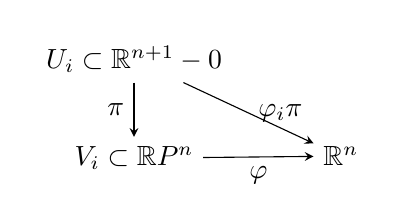
\begin{tikzpicture}
  \matrix (m) [matrix of math nodes, row sep=2em, column sep=3em, minimum width=1em]
  {
    U_i \subset \mathbb{R}^{n+1} - 0 &  \\
    V_i \subset \mathbb{R}P^n  & \mathbb{R}^n  \\ };
  \path[-stealth]
  (m-1-1) edge node [right] {$\varphi_i \pi$} (m-2-2)
  edge node [left] { $\pi$} (m-2-1)
  (m-2-1) edge node [below] {$\varphi$} (m-2-2);
\end{tikzpicture}

\[
\begin{gathered}
  \begin{aligned}
    & \varphi_i : U_i \subset \mathbb{R}P^n \to \mathbb{R}^n \\ 
    & \varphi_i[x^1 \dots x^{n+1} ] = \left( \frac{x^1}{x^i} \dots \frac{ \widehat{x}^i }{ x^i } \dots \frac{x^{n+1}}{ x^i } \right) \\
    & \varphi^{-1}_i(u^1 \dots u^n) = [ u^1 \dots u^{i-1}, 1 , u^i \dots u^n ]
\end{aligned} \\ 
  \varphi_i^{-1} \varphi_i[x^1 \dots x^{n+1} ] = \left[ \frac{x^1 }{ x^i } \dots \frac{x^{i-1}}{ x^i } , 1 , \frac{x^{i+1}}{ x^i} \dots \frac{x^{n+1}}{ x^i } \right] = [x^1 \dots x^{i-1}, x^i , x^{i+1} \dots x^{n+1} ] \\
  \varphi_i \varphi^{-1}_i(u^1 \dots u^n) = (u^1 \dots u^{i-1} , u^i  \dots u^n )
\end{gathered}
\]
cont. $\varphi_i$ bijective, $\varphi_i^{-1}$ cont. $\varphi_i$ homeomorphism.  

From a previous edition: 

\exercisehead{1.2} 


Let $ \begin{aligned} & \quad \\ 
  & \phi_t : \mathbb{R}^{n+1}\backslash \lbrace  0 \rbrace \to \mathbb{R}^{n+1} \backslash \lbrace 0 \rbrace \\ 
  & \phi_t(x) = tx \end{aligned}$ \\
$\phi_t$ invertible, $\phi_t^{-1} = \phi_{\frac{1}{t}}$ \\
$\phi_t$, $\phi_t^{-1}$ \, $C^1$ (and $C^{\infty}$), $\phi_t$ homeomorphism.  \\

Let $U$ open in $\mathbb{R}^{n+1}\backslash \lbrace 0 \rbrace$.  Then $\phi_t(U)$ open in $\mathbb{R}^{n+1}\backslash \lbrace 0 \rbrace$.  \\
Thus $\pi^{-1}([U]) = \bigcup_{t \in \mathbb{R}} \phi_t(U)$ open in $\mathbb{R}^{n+1}\backslash \lbrace 0 \rbrace$.  \\
Thus $[U]$ open in $\mathbb{R}P^n$.  $\sim$ open.  \\

Note $\begin{aligned} & \quad  \\
  & \pi : \mathbb{R}^{n+1} \backslash \lbrace 0 \rbrace \to \mathbb{R}P^n \\
  & \pi(x) = \frac{x}{ \| x\| } \end{aligned}$ \\
$\mathbb{R}^n$ 2nd. countable, $\mathbb{R}P^n$ 2nd. countable.  


\exercisehead{1.3}

$S^n$ compact. \\
$\pi :\mathbb{R}^{n+1}\backslash \lbrace 0 \rbrace \to \mathbb{R}P^n$ \\
$\pi(x) = [ \frac{x}{ \| x \| } ]$ \\
Let $x \in \mathbb{R}P^n$ \\
\phantom{Let } $y = \frac{x}{ \| x \| } \in S^n$ and $ \left. \pi \right|_{S^n}(y) = [x]$ \\
$\left. \pi \right|_{S^n}$ surjective.  



\exercisehead{1.6}

First, note that $\sim $ on $\mathbb{R}^{n+1} -0$ in the definition of $\mathbb{R}P^n$ is an open $\sim$ i.e. open equivalence relation.  

This is because of the following:
$\forall \, U \subset \mathbb{R}^{n+1}-0$, \\
$\pi^{-1}(\pi(U)) = \bigcup_{t\in \mathbb{R}} tU$, set of all pts. equivalent to some pt. of $U$.  \\
multiplication by $t\in \mathbb{R}$ homeomorphism of $\mathbb{R}^{n+1} - 0$, so $tU$ open $\forall \, t \in \mathbb{R}$.  \\
$\pi^{-1}(\pi(U))$ open i.e. $\pi(U)$ open (for $\pi$ is cont.).  


Let $X = \mathbb{R}^{n+1} -0$.  \\
Consider $R = \lbrace ( x,y) \in X \times X | x\sim y \text{ or } y = tx \text{ for some } t \in \mathbb{R} \rbrace$ 

$y = tx$ means $y_i = tx_i$ \, $\forall \, i = 0\dots n$.  Then $\frac{ x_i}{y_i} = \frac{ x_j}{ y_j}$ \, $\forall \, i,j = 0 \dots n$.  Hence $x_i y_j - y_i x_j = 0$ \, $\forall \, i , j$.  

Let $\begin{aligned} & \quad \\ 
  & f : X \times X \to \mathbb{R} \\
  & f(x,y) = \sum_{ i \neq j} (x_i y_j - y_i x_j)^2 \end{aligned}$  

\[
\begin{aligned}
  & \frac{ \partial f}{ \partial x_i} = \sum_{i \neq j } 2 (x_i y_j - y_i x_j) ( y_j - y_j) = 0 \\
  & \frac{ \partial f}{ \partial y_j} = \sum_{j \neq i } 2 (x_i y_j - y_i x_j) ( x_i - x_i) = 0 
\end{aligned}
\]

Nevertheless, $f$ is $C^1$ so $f$ cont.  

So $f^{-1}(0) = R$. 

$0$ closed, so $f^{-1}(0) = R$ closed.  By theorem, since $\sim$ open, $\mathbb{R}P^n = \mathbb{R}^{n+1} - 0 / \sim$ Hausdorff.  

cf. \url{http://math.stackexchange.com/questions/336272/the-real-projective-space-rpn-is-second-countable}

topological space is second countable if its topology has countable basis.  \\
\quad $\mathbb{R}^n$ second countable since $\mathcal{B} = \lbrace B_r{ ( q)} | r,q \in \mathbb{Q} \rbrace$ is a countable basis.  $\forall \, x \in \mathbb{R}^n$ \\

If $X$ is second countable, with countable basis $\mathcal{B}$, 
\begin{enumerate}
\item If $Y \subseteq X$, $Y$ also second countable with countable basis $\lbrace B | B \in \mathcal{B}, \, Y \bigcap B \neq \emptyset \rbrace$
\item If $Z == X/\sim $, $\lbrace \lbrace [x] | x \in B \rbrace | B \in \mathcal{B} \rbrace$ is a countable basis for $Z$ since $\mathcal{B}$ countable.  \\

It is a basis since 

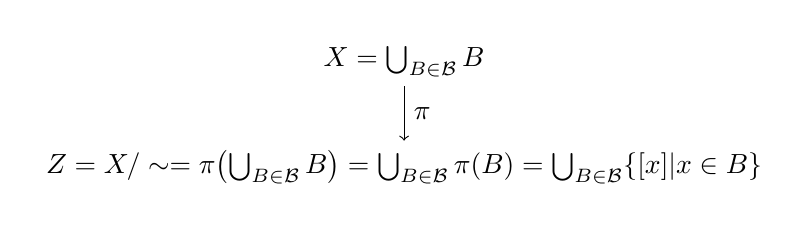
\begin{tikzpicture}
  \matrix (m) [matrix of math nodes, row sep=2em, column sep=3em, minimum width=1em]
  {
X = \bigcup_{B \in \mathcal{B}} B    \\
Z = X/ \sim = \pi{ \left( \bigcup_{B \in \mathcal{B}} B \right) } = \bigcup_{B \in \mathcal{B}} \pi{ (B)} = \bigcup_{ B \in \mathcal{B}} \lbrace [x] | x  \in B \rbrace \\
  };
%  \path[-stealth]
  \path[->]
  (m-1-1) edge node [right] {$\pi$} (m-2-1);
\end{tikzpicture}


\end{enumerate}

Now let $Y = \mathbb{R}^n-0$ and \\
\phantom{Now let } $Z = \mathbb{R}P^n = \mathbb{R}^n-0 / \sim$

\exercisehead{1.7}

$S^n$ compact so $S^n/\lbrace \pm \rbrace$ compact by Theorem, as $\pi_S(S^n) = S^n/ \lbrace \pm \rbrace$, as $\pi_S$ cont. surjective ($\forall \, [x] \in S^n/\lbrace \pm \rbrace$, $\exists \, x \in S^n$ s.t. $\pi_S(S^n) = [x]$) \\
$g$ cont. bijective as defined above so since $g(S^n/\lbrace \pm \rbrace) = \mathbb{R}P^n$, $\mathbb{R}P^n$ compact.  


\textbf{Example 1.8 (Product Manifolds)}
\[
\begin{aligned}
  & M_1 = \bigcup_{\alpha \in \mathfrak{A}_1} U_{\alpha}^{(1)} \\ 
  & M_i = \bigcup_{\alpha \in \mathfrak{A}_i} U_{\alpha}^{(i)} 
\end{aligned} \quad \quad \quad \, 
M_1 \times \dots \times M_n = \bigcup_{ \begin{aligned} & \alpha_1 \in \mathfrak{A}_1 \\ 
& \vdots \\ 
    & \alpha_n \in \mathfrak{A}_n \end{aligned} }  U_{\alpha_1} \times \dots \times U_{\alpha_n} \quad \quad \, (\text{by def.})
\]

$\forall \, p = (p_1 \dots p_n) \in M_1 \times \dots M_n$, consider $p_i \in M_i$.  Choose coordinate chart $(U_{j_i}, \varphi_{j_i})$, $\varphi_i(U_i) \subset \mathbb{R}^{n_i}$.  Then,  \\

Consider $\varphi : U_1 \times \dots \times U_n \to \mathbb{R}^{m_1} \times \dots \times \mathbb{R}^{m_n} = \mathbb{R}^{ m_1 + \dots + m_n}$, $(U_1 \times \dots \times U_n, \varphi_1 \times \dots \times \varphi_n)$ \\
$\varphi = \varphi_1 \times \dots \times \varphi_n$\\
$\varphi$ also a homeomorphism.  $\begin{gathered} \varphi \psi^{-1} \\ (\varphi_1 \times \dots \times \varphi_n) \circ(\psi_1 \times \dots \times \psi_n)^{-1} \end{gathered}$ also a diffeomorphism, cont. bijective and $C^{\infty}$ \\
$\lbrace (U, \varphi)  = (U_1 \times \dots \times U_n, \varphi_1 \times \dots \times \varphi_n) | (U_i, \varphi_i) \in \lbrace (U_i, \varphi_i) | U_i \in M_i \rbrace \rbrace$ also an atlas.  



\subsubsection*{Topological Properties of Manifolds}

\begin{lemma}[1.10]
$\forall \, $ topological $M$, $M$ has countable basis of precompact coordinate balls
\end{lemma}

\begin{proof}
  First consider $M$ can be covered by single chart.  \\
Suppose $\varphi : M \to \widehat{U} \subseteq \mathbb{R}^n$ global coordinate map. \\
Let $\mathcal{B} = \lbrace B_r(x) | \text{ open } B_r(x) \subseteq \mathbb{R}^n \text{ s.t. } r\in \mathbb{Q}, \, x \in \mathbb{Q}, \, \text{ i.e. $x$ rational coordinates }, B_{r'}(x) \subseteq \widehat{U}, \text{ for some } r' > r \rbrace$ \\
Clearly, $\forall \, B_r(x)$ precompact in $\widehat{U}$ \\
\quad \, $\mathcal{B}$ countable basis for topology of $\widehat{U}$

$\varphi$ homeomorphism, it follows $\lbrace \varphi^{-1}(B) | B \in \mathcal{B} \rbrace$ countable basis for $M$

Let $M$ arbitrary, \\
\quad By def., $\forall \, p \in M$, $p \in $ domain $U$ of a chart

Prop. A.16, $\forall \, $ open cover of second-countable space has countable subcover. \\
\quad $M$ covered by countably many charts $\lbrace (U_i, \varphi_i) \rbrace$ \\
$\forall \, U_i$, $U_i$ has countable basis of coordinate balls precompact in $U_i$ \\
union of all these coordinates bases is countable basis for $M$.   \\

If $V \subseteq U_i$ one of these balls,  \\
\quad then $\overline{V}$ compact in $U_i$.  $M$ Hausdorff, so $\overline{V}$ closed.  \\
\quad $\overline{V}$ in $M$ is same as $\overline{V}$ in $U_i$, so $V$ precompact in $M$.   
\end{proof}

\subsubsection*{Connectivity}

\subsubsection*{Local Compactness and Paracompactness}



\subsubsection*{Fundamental Groups of Manifolds}





\subsection*{Smooth Structures}

If open $U \subset \mathbb{R}^n$, $V \subset \mathbb{R}^m$, \\
$F:U \to V$ smooth (or $C^{\infty}$) if $\forall \, $ cont. partial derivative of all orders exists.  \\

$F$ diffeomorphism if $F$ \emph{smooth}, bijective, and has a \emph{smooth} inverse.  \\
Diffeomorphism is a homeomorphism.  \\

$(U, \varphi), (V,\psi)$ smoothly compatible if $UV = \emptyset$ or 
\[
\psi \varphi^{-1}: \varphi(UV) \to \psi(UV) \quad \quad \, \text{ diffeomorphism }
\]

atlas $\mathcal{A} \equiv \lbrace (U, \varphi ) \rbrace$ s.t. $\bigcup U = M$.  Smooth atlas if $\forall \, (U,\varphi), (V, \psi) \in \mathcal{A}$, $(U,\varphi), (V,\psi)$ smoothly compatible.  \\

Smooth structure on topological $n$-manifold $M$ is a maximal smooth atlas.   \\

Smooth manifold $(M, \mathcal{A})$ where $M$ topological manifold, $\mathcal{A}$ smooth structure on $M$.   \\


\begin{proposition}[1.17] Let $M$ topological manifold. 
\begin{enumerate}
\item[(a)] $\forall \, $ smooth atlas for $M$ is contained in ! maximal smooth atlas.  
\item[(b)] 2 smooth atlases for $M$ determine the same maximal smooth atlas iff union is smooth atlas.  
\end{enumerate}
\end{proposition}

\begin{proof}
Let $\mathcal{A}$ smooth atlas for $M$   \\
$\overline{ \mathcal{A} } \equiv $ set of all charts that are smoothly compatible with every chart in $\mathcal{A}$ 

\textbf{Want}: $\overline{ \mathcal{A}}$ smooth atlas, i.e. $\forall \, (U, \varphi), (V \psi) \in \overline{\mathcal{A}}$, $\psi \varphi^{-1} : \varphi(UV) \to \psi(UV)$ smooth.  

Let $x = \varphi(p) \in \varphi(UV)$ \\
$p\in M$, so $\exists \,$ some chart $(W, \theta) \in \mathcal{A}$ s.t. $p \in W$.  \\
By given, $\theta \varphi^{-1}, \psi \theta^{-1}$ smooth where they're defined.   \\
$p \in UVW$, so $\psi \varphi^{-1} = \psi \theta^{-1} \theta \varphi^{-1}$ smooth on $x$.  \\
Thus $\psi \varphi^{-1}$ smooth in a neighborhood of each pt. in $\varphi(UV)$.  Thus $\overline{\mathcal{A}}$ smooth atlas.  

To check maximal, 


\end{proof}




\subsection*{Local Coordinate Representations}

\begin{proposition}[1.19]
  $\forall \, $ smooth $M$ has countable basis of regular coordinate balls
\end{proposition}

\exercisehead{1.20}

smooth manifold $M$ has smooth structure \\
\quad Suppose single smooth chart $\varphi$ has entire $M$ as domain
\[
\varphi: M \to \widehat{U} \subseteq \mathbb{R}^n
\]

Let $\widehat{B} = \lbrace \widehat{B}_r(x) \subseteq \mathbb{R}^n | r \in \mathbb{Q}, \, x \in \mathbb{Q}, \, \widehat{B}_{r'}(x) \subseteq \widehat{U} \text{ for some } r' > r \rbrace$ \\

\quad $\forall \, \widehat{B}_r(x)$ precompact in $\widehat{U}$ \\
\quad $\widehat{\mathcal{B}}$ countable basis for topology of $\widehat{U}$

$\varphi$ homeomorphism, 

\quad Let $\begin{aligned}
  & \quad \\
  & \varphi^{-1}( \widehat{B}_r{(0)}) = B \\
  & \varphi^{-1}{(\widehat{B}_{r'}{(0)} )} = B' \end{aligned}$

$\varphi$ homeomorphism and since $\widehat{B}$ countable basis, $\lbrace B \rbrace$ countable basis of regular coordinate basis. \\

Suppose arbitrary smooth structure.  \\
\quad By def., $\forall \, p \in M$, $p$ in some chart domain \\
\quad Prop. A.16., $\forall \, $ open cover of second countable space has countable subcover \\
\quad $M$ covered by countably many charts $\lbrace (U_i, \varphi_i) \rbrace$ \\

$\forall \, U_i , \, U_i$ has countable basis of coordinate balls precompact in $U_i$ \\
union of all these coordinate charts is countable basis for $M$.  

If $V \subseteq U_i$, 1 of these balls,  \\
$\begin{aligned}
  & \quad \\ 
  & \varphi(V) = B_r(0) \\ 
  & \varphi{(\overline{V})} = \overline{B}_r(0)
\end{aligned}$

and $\varphi(B') = B_{r'}{(0)}$, $r' > r$ for countable basis for $U_i$ \\
So $V$ regular coordinate ball.


\hrulefill



\subsection*{Examples of Smooth Manifolds}






\subsubsection*{More Examples}



\textbf{Example 1.25 (Spaces of Matrices) } Let $M(m\times n,\mathbb{R}) \equiv $ set of $m\times n$ matrices with real entries.  

\textbf{Example 1.26 (Open Submanifolds)}

$\forall \, $ open subset $U \subseteq M$ is itself a $\text{dim}{M}$ manifold. \\
EY : \emph{ $\forall \, $ open subset $U \subseteq M$ is itself a $\text{dim}{M}$ manifold. }


\textbf{Example 1.27 (The General Linear Group) }

general linear group $GL(n,\mathbb{R}) = \lbrace A | \text{det}{A} \neq 0 \rbrace$ \\
\quad $\text{det}:A \to \mathbb{R}$ is cont. (by def. of $\text{det}{A} = \epsilon^{ i_1 \dots i_n}a_{1 i_1} \dots a_{n i_n}$ \\
\quad $\text{det}^{-1}{ ( \mathbb{R} - 0 )}$ is open since $\mathbb{R}-0$ open so $GL(n,\mathbb{R})$ open \\
\quad $GL(n,\mathbb{R}) \subseteq M(n,\mathbb{R})$, $M(n,\mathbb{R})$ $n^2$-dim. vector space. \\
\quad \quad so $GL(n,\mathbb{R})$ smooth $n^2$-dim. manifold.  

\textbf{Example 1.28 (Matrices of Full Rank)}

Suppose $m <n$ \\

Let $M_n(m\times n, \mathbb{R}) \subseteq M(m\times n, \mathbb{R})$ with matrices of rank $m$ \\
if $A \in M_m(m\times n, \mathbb{R})$, \\
\quad $\text{rank}{A}=m$ 

means that $A$ has some nonsingular $m \times m$ submatrix.  (EY 20140205 ???)




\textbf{Example 1.31 (Spheres)} 

\[
\begin{aligned}
  & \varphi_i^{\pm} : S^n \to B_1^n(0) \subset \mathbb{R}^n \quad \, (B_1^n(0) \text{ disk of radius $1$}) \\
  & \varphi_i^{\pm}(x_1 \dots x_{n+1}) = (x_1 \dots \widehat{x}_i \dots x_{n+1} )= (y_1 \dots y_n)
\end{aligned}
\]
Note $x_1^2 + \dots + x_i^2 + \dots + x_{n+1}^2 = 1$.  \quad \, $x_i = \pm \sqrt{ 1 - (x_1^2 + \dots + \widehat{x}_i^2 + \dots + x_{n+1}^2 ) }$

\[
\begin{aligned}
  & (\varphi_i^{\pm})^{-1}(y_1 \dots y_n) = (y_1 \dots \pm \sqrt{ 1 - (y_1^2 + \dots + y_n^2) } \dots y_n) = (y_1 \dots y_{i-1}, \pm \sqrt{ 1-  |y|^2 }, y_i\dots y_n ) \\ 
 & \varphi_i^{\pm} (\varphi_j^{\pm})^{-1}(y_1 \dots y_n ) = (y_1 \dots \widehat{y}_i \dots y_{j-1} , \pm \sqrt{ 1 - |y|^2 }, y_j \dots y_n) \\ 
 & \varphi_i^{\pm} (\varphi_j^{\mp})^{-1}(y_1 \dots y_n ) = (y_1 \dots \widehat{y}_i \dots y_{j-1} , \mp \sqrt{ 1 - |y|^2 }, y_j \dots y_n) \\ 
\end{aligned}
\]
\[
\varphi_j^{\pm}(\varphi_i^{\mp})^{-1} \varphi_i^{\pm} (\varphi_j^{\pm})^{-1}(y_1 \dots y_n) = \varphi_j^{\pm}(y_1 \dots \pm y_i \dots y_{j-1}, \pm \sqrt{ 1 - |y|^2 } \dots y_n ) = (y_1 \dots \pm y_i \dots y_j \dots y_n)
\]
This is symmetrical in $i,j$ and so true if $i,j$ reverse.  \\

So $\varphi_i^{\pm}(\varphi_j^{\pm})^{-1}$ diff. and bijective.  Likewise for $\varphi_i^{\pm}(\varphi_j^{\mp})^{-1}$.  \\
So $\begin{aligned} & \varphi_i^{\pm} (\varphi_j^{\pm})^{-1} \\ 
  & \varphi_i^{\pm} (\varphi_j^{\mp})^{-1} \end{aligned}$ diffeomorphisms.  

\begin{lemma}[1.35] \textbf{(Smooth Manifold Chart Lemma)}
Let $M$ be a set, suppose given $\lbrace U_{\alpha} | U_{\alpha} \subset M \rbrace$, given maps $\varphi_{\alpha}: U_{\alpha} \to \mathbb{R}^n$ s.t.
\begin{enumerate}
\item[(i)] $\forall \, \alpha$, $\varphi_{\alpha}$ bijection between $U_{\alpha}$ and open $\varphi_{\alpha}(U_{\alpha}) \subseteq \mathbb{R}^n$
\item[(ii)] $\forall \, \alpha, \beta$, $\varphi_{\alpha}(U_{\alpha} \bigcap U_{\beta})$, $\varphi_{\beta}(U_{\alpha} \bigcap U_{\beta})$ open in $\mathbb{R}^n$
\end{enumerate}
\end{lemma}


\textbf{Example 1.36 (Grassmann Manifolds)}

%$G_k(V) = $ set of all $k$-dim. linear subspaces of $V$, $\text{dim}{V} = n \geq k $

%Let $P,Q$ complementary subspaces of $V$, $\begin{aligned} & \quad \\ & \text{dim}{P} = k \\ & \text{dim}{Q} = n- k \end{aligned}$

%direct sum decomposition $V = P \oplus Q$  

%graph of any linear $X: P \to Q$

%\[
%\Gamma(X) = \lbrace v + X v | v \in P \rbrace \subset V
%\]
%$k$-dim. subspace

%Now $\Gamma(X) Q = \emptyset$ since $\Gamma(A) \subset P \oplus Q$ and $P$ and $Q$ are complementary.  

%If $KQ = \emptyset$, then $K \subset P \oplus Q$, $P\neq 0$.  

$G_k(V) = \lbrace S | S \subseteq V \rbrace$ \quad \, $S$ $k$-dim. linear subspace of $V$ \\
$\text{dim}V = n$, $V$ vector space  \\

if $V = \mathbb{R}^n$, $G_k(\mathbb{R}^n) \equiv G_{k,n} \equiv G(k,n)$ (notation) \quad \, $G_1(\mathbb{R}^{n+1}) = \mathbb{R}P^n$

Let $V = P \oplus Q$, \, $\begin{aligned}
  & \text{dim}P =k \\
  & \text{dim}Q = n-k \end{aligned}$ \\

linear $X: P \to Q$ 

\[
\Gamma(X) = \lbrace v + Xv | v \in P \rbrace , \quad \, \Gamma(X) \subseteq V, \, \text{dim}\Gamma(X) = k
\]
$\Gamma(X) \bigcap Q = 0$ since $\forall \, w \in \Gamma(X)$, $w$ has a $P$ piece, and $Q$ complementary to $P$ \\

Converse: $\forall \, $ subspace $S \subseteq V$, s.t. $S\bigcap Q = 0$ \\
\quad \, let $\begin{aligned}
  & \quad \\ 
  & \pi_P : V \to P \\ 
  & \pi_Q: V \to Q
\end{aligned}$ \quad \, projections by direct sum decomposition $V = P\oplus Q$ \\

$\left. \pi_P \right|_S : S \to P$ isomorphism  \\
$\Longrightarrow X = ( \left. \pi_Q \right|_S ) \cdot ( \left. \pi_P \right|_S)^{-1}$, \, $X: P \to Q$ \\

Let $v\in P$.  $v+ Xv = v +  \left. \pi_Q \right|_S (  \left. \pi_P \right|_S)^{-1} v$.  Let $v  \in \left. \pi_P \right|_S (S)$ \quad \, $\Gamma(X) = S$ \\


Let $L(P;Q) = \lbrace f | \text{ linear } f : P \to Q \rbrace$, \, $L(P;Q)$ vector space \\
$U_Q \subseteq G_k(V)$, \, $U_Q = \lbrace S | \text{dim}S =k, \, S \text{ subspace }, \, S \bigcap Q = 0 \rbrace$ \\
$\begin{aligned}
  & \Gamma : L(P;Q) \to U_Q \\
  & X \mapsto \Gamma(X) \end{aligned}$ \\

$\Gamma$ bijection by above \\
$\varphi = \Gamma^{-1} : U_Q \to L(P;Q)$  \\

By choosing bases for $P,Q$, identify $L(P;Q)$ with $M((n-k)k; \mathbb{R})$ and hence with $\mathbb{R}^{k(n-k)}$ \\

think of $(U_Q, \varphi)$ as coordinate chart. \\
$\varphi(U_Q) = L(P;Q)$













\subsection*{Problems}

\problemhead{1.7} (This was Problem 1.5 in previous editions)

\[
S^n = \lbrace ( x_1 \dots x_{n+1} \rbrace \in \mathbb{R}^{n+1} | \sum_{i=1}^{n+1} x_i^2 = 1 \rbrace \subset \mathbb{R}^{n+1}
\]

Let $\begin{aligned} & \quad \\
  & N = (0 \dots 0, 1) \\ 
  & S = (0 \dots 0, -1) \end{aligned}$ \quad \, $x\in S^n$. 
\begin{enumerate}
\item[(a)]
 Consider $t(x-N) + N = tx + (1-t)N$ when $x_{n+1} =0$ 
\[
\begin{gathered}
  tx_{n+1} + (1-t) = 0 \text{ or } tx_{n+1} + -1 + t = 0 \\ 
  \Longrightarrow \frac{ 1}{ 1- x_{n+1} } = t \quad \left( \text{ or } \frac{1}{ 1 + x_{n+1} } \right)
\end{gathered}
\]

\[
\begin{aligned}
  & \pi_1: S^n - N \to \mathbb{R}^n \\ 
  & \pi_1(x_1 \dots x_{n+1}) = \left( \frac{x_1}{ 1 - x_{n+1} } \dots \frac{x_n}{ 1 - x_{n+1} } , 0 \right) \\ 
  & \pi_2 : S^n -S \to \mathbb{R}^n \\ 
  & \pi_2(x_1 \dots x_{n+1}) = \left( \frac{x_1}{ 1 + x_{n+1}} \dots \frac{x_n}{ 1 + x_{n+1} }, 0 \right)
\end{aligned}
\]
Note that $-\pi_2(-x) = \pi_1$ and $\pi_1 \equiv \sigma$, $\pi_2 \equiv \widetilde{\sigma}$ in Massey's notation.  
\item[(b)] Note, for $y_i = \frac{x_i}{ 1 - x_{n+1}}$
\[
\begin{gathered}
  y_1^2 + \dots +y_n^2 = |y|^2 = \frac{1-  x_{n+1}^2}{ (1-x_{n+1})^2 } = \frac{1+ x_{n+1}}{ 1- x_{n+1}} \text{ or } x_{n+1}  = \frac{ |y|^2 - 1 }{ |y|^2 + 1 }  \\
  x_i = y _i (1- x_{n+1}) = \frac{2y_i}{ 1 + |y|^2 }
\end{gathered}
\]

\[
\begin{aligned}
  & \pi_1^{-1}: \mathbb{R}^n \to S^n - N \\ 
  & \pi_1^{-1}(y_1 \dots y_n) = \left( \frac{2y_1}{ 1 + |y|^2 } \dots \frac{2y_n}{1+ |y|^2 } , \frac{ |y|^2 - 1 }{ |y|^2 + 1 } \right) \\ 
  & \pi_2^{-1}(y_1 \dots y_n) = \left( \frac{2y_1}{ 1 + |y|^2 } \dots \frac{2y_n}{1+ |y|^2 } , \frac{ 1 - |y|^2  }{ |y|^2 + 1 } \right)
\end{aligned}
\]

$\pi_1,\pi_2$ diff., bijective, and $(S^n - N ) \bigcup (S^n-S) = S^n$ \\

\item[(c)] Computing the transition maps for the stereographic projections.


Consider $(S^n - N)(S^n-S) = S^n - N \bigcup S$ 
\[
\begin{aligned}
  & \pi_1 \pi_2^{-1}(y_1 \dots y_n) = \left( \frac{y_1 }{ |y|^2} \dots \frac{y_n}{|y|^2} , 0 \right) \\ 
  & \pi_2 \pi_1^{-1}(y_1 \dots y_n) = \left( \frac{y_1 }{ |y|^2} \dots \frac{y_n}{|y|^2} , 0 \right) 
\end{aligned}
\]
since, for example, 
\[
\begin{gathered}
\frac{   \frac{2y_i }{ 1 + |y|^2} }{ 1 - \frac{ 1 - |y|^2}{ 1 + |y|^2 }} = \frac{y_i }{ |y|^2 }
\end{gathered}
\]



$\pi_1 \pi_2^{-1}$ bijective and $C^{\infty}$, $\pi_1 \pi_2^{-1}$ diffeomorphism.   \\

$\lbrace (S^n-N, \pi_1), (S^n - S, \pi_2) \rbrace$ \, $C^{\infty}$ atlas or differentiable structure.  
\[
\begin{aligned}
  & \partial_j \frac{y_i}{ |y|^2} = \frac{ - 2y_i y_j }{ (y_1^2 + \dots + y_n^2 )^2 } \\ 
  & \partial_j \frac{ y_j}{ |y|^2} = \frac{ (y_1^2 + \dots + y_n^2) - 2y_j^2 }{ |y|^4} = \frac{ y_1^2 + \dots + \widehat{y}_j^2 + \dots + y_n^2 - y_j^2 }{ |y|^4}
\end{aligned}
\]
\[
\text{det}{ (\partial_j \pi_1 \pi_2^{-1}(y) ) } = \sum_{ \sigma \in S_n} \text{sgn}{ (\sigma)} \partial_{\sigma_1} \frac{y_1}{ |y|^2} \dots \partial_{\sigma_n} \frac{y_n}{|y|^2} = 0 \text{ only if $y=0$. But that's excluded }
\]
\item[(d)] Consider $\begin{gathered}
  \lbrace ( S^n\backslash, \pi_1), (S^n \backslash S, \pi_2) \rbrace \\ 
  \mathcal{A} = \lbrace (U_i^{\pm}, \varphi_i^{\pm}) \rbrace \end{gathered}$  \\

Now 
\[
\begin{aligned}
  & S^n \backslash N \bigcap U_i^+ = \begin{cases} U_i^+ & \text{ if } i \neq n + 1 \\ U_{n+1}^+ \backslash N & \text{ if } i = n+1 \end{cases} \\ 
  & S^n \backslash N \bigcap U_i^- = U_i^-
\end{aligned}
\]

\[
\pi_1(\varphi_i^{\pm})^{-1}(y_1 \dots y_n) = \pi_1(y_1 \dots y_{i-1}, \pm \sqrt{ 1 - |y|^2 }, y_i \dots y_n) = \left( \frac{y_1 }{ 1 - y_n} \dots \frac{y_{i-1} }{ 1 - y_n}, \frac{ \pm \sqrt{ 1 - |y|^2 } }{ 1 - y_n } , \frac{y_i}{ 1 - y_n} \dots \frac{y_{n-1}}{ 1 - y_n }, 0 \right)
\]

Note $-1< y_n <1$ on $\varphi_i^{\pm}(S^n\backslash \bigcap U_i^{\pm})$
\[
\varphi_i^{\pm} \pi_1^{-1}(y_1 \dots y_n) = \varphi_i^{\pm}\left( \frac{ 2y_1}{ 1 + |y|^2} \dots \frac{2y_n}{ 1 + |y|^2} , \frac{|y|^2 - 1 }{ |y|^2 + 1 } \right) = \left( \frac{2y_1 }{ 1 + |y|^2} \dots \frac{ 2 \widehat{y}_i }{ 1 + |y|^2 } \dots \frac{ 2y_n }{ 1 + |y|^2 }, \frac{|y|^2 -1}{ |y|^2 + 1 } \right)
\]
$\pi_{1,2}(\varphi_i^{\pm})^{-1}, \varphi_i^{\pm}\pi_{1,2}^{-1}$ are diffeomorphisms (bijective and differentiable).  

So $\lbrace(S^n\backslash N, \pi_1), (S^n\backslash S , \pi_2) \rbrace \bigcup \mathcal{A}$ also a $C^{\infty}$ atlas.  \\
So $\lbrace(S^n\backslash N, \pi_1), (S^n\backslash S , \pi_2) \rbrace$ ,  $\mathcal{A}$ equivalent.  



\end{enumerate}





\section{Smooth Maps}
% 02smoothmaps.tex
% Fund Science! & Help Ernest finish his Physics Research! : quantum super-A-polynomials - a thesis by Ernest Yeung
%                                               
% http://igg.me/at/ernestyalumni2014                                                                             
%                                                              
% Facebook     : ernestyalumni  
% github       : ernestyalumni                                                                     
% gmail        : ernestyalumni                                                                     
% google       : ernestyalumni                                                                                   
% linkedin     : ernestyalumni                                                                             
% tumblr       : ernestyalumni                                                               
% twitter      : ernestyalumni                                                             
% youtube      : ernestyalumni                                                                
% indiegogo    : ernestyalumni                                                                        
%
% Ernest Yeung was supported by Mr. and Mrs. C.W. Yeung, Prof. Robert A. Rosenstone, Michael Drown, Arvid Kingl, Mr. and Mrs. Valerie Cheng, and the Foundation for Polish Sciences, Warsaw University.                  
 

\subsection*{Smooth Functions and Smooth Maps}

\begin{definition}
 \textbf{smooth function } $f$, $f:M \to \mathbb{R}^k$, if $\forall \, p \in M$,  $\exists \, $ smooth chart $(U,\varphi)$, $U \ni p$, s.t. $f\circ \varphi^{-1}$ smooth on $\varphi(U) \subseteq \mathbb{R}^n$, $f\circ \varphi^{-1}: \varphi(U) \to \mathbb{R}^k$
\end{definition}
EY : 20150717 Recall, smooth chart just means that the chart belongs to maximal smooth atlas, and smooth in that the transition maps are smooth.  

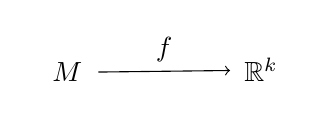
\begin{tikzpicture}
  \matrix (m) [matrix of math nodes, row sep=3.8em, column sep=4.8em, minimum width=2.2em]
  {
M & \mathbb{R}^k \\
};
  \path[->]
  (m-1-1) edge node [above] {$f$} (m-1-2)
  ;
\end{tikzpicture} 

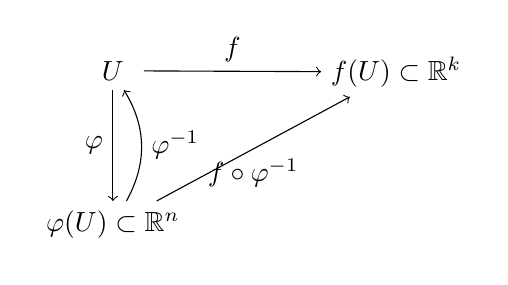
\begin{tikzpicture}
  \matrix (m) [matrix of math nodes, row sep=3.8em, column sep=4.8em, minimum width=2.2em]
  {
U & f(U) \subset \mathbb{R}^k  \\
\varphi(U) \subset \mathbb{R}^n &    \\
};
  \path[->]
  (m-1-1) edge node [above] {$f$} (m-1-2)
          edge node [left] {$\varphi$} (m-2-1)
  (m-2-1) edge [bend right] node [right] {$\varphi^{-1}$} (m-1-1)
          edge node [below] {$f\circ \varphi^{-1}$} (m-1-2)
          ;
\end{tikzpicture} 



\exercisehead{2.3} Given $f: M \to \mathbb{R}^k$ smooth, \\
Consider $p \in M$.  $M$ smooth manifold, so $\exists \, $ chart $(U,\varphi)$ s.t. $p \in U$ \\
$\varphi : U \subset M \to \mathbb{R}^m$ \\
$\varphi$ homeomorphism, $\varphi(U)$ open in $\mathbb{R}^m$  
$\varphi^{-1}: \varphi(U) \to M$

Consider another smooth chart $(V,\psi)$, $p\in V$ so that $UV \neq \emptyset$
\[
\begin{gathered}
  f\psi^{-1} : \psi(UV) \to \mathbb{R}^k \\ 
  f\psi^{-1}(y^1 \dots y^m ) = (f\psi^{-1})_i(y^1 \dots y^m) , \quad \, i = 1\dots k \\
  f\psi^{-1} = f\varphi^{-1}\varphi \psi^{-1} = (f\varphi^{-1}) \varphi \psi^{-1}
\end{gathered}
\]
$\varphi \psi^{-1}$ $C^{\infty}$ (diffeomorphisms are smooth).  $f\varphi^{-1}$ is smooth.  $f\psi^{-1}$ also smooth.  

\subsubsection*{Smooth Maps Between Manifolds}

\begin{definition}
  Let $M,N$ be smooth manifolds.  \\
  \textbf{smooth map } $F$, $F:M \to N$ if $\forall \, p \in M$, $\exists \, $ smooth charts $\begin{aligned} & \quad \\
    & (U,\varphi) \quad \, U \ni p \\
    & (V,\psi) \quad \, V \ni F(p) \end{aligned}$

s.t. $F(U) \subseteq V$ and \\
\phantom{s.t. } $\psi \circ F \circ \varphi^{-1}$ smooth from $\varphi(U)$ to $\psi(V)$.  
\end{definition}

i.e. 


\begin{tikzpicture}
  \matrix (m) [matrix of math nodes, row sep=3.8em, column sep=4.8em, minimum width=2.2em]
  {
M &  N \\
};
  \path[->]
  (m-1-1) edge node [above] {$F$} (m-1-2)
  ;
\end{tikzpicture} 

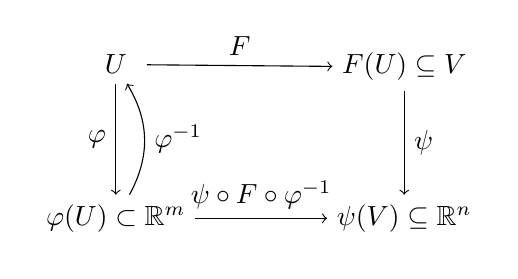
\begin{tikzpicture}
  \matrix (m) [matrix of math nodes, row sep=3.8em, column sep=4.8em, minimum width=2.2em]
  {
U & F(U) \subseteq V  \\
\varphi(U) \subset \mathbb{R}^m & \psi(V) \subseteq \mathbb{R}^n    \\
};
  \path[->]
  (m-1-1) edge node [above] {$F$} (m-1-2)
          edge node [left] {$\varphi$} (m-2-1)
  (m-1-2) edge node [auto] {$\psi$} (m-2-2)
  (m-2-1) edge [bend right] node [right] {$\varphi^{-1}$} (m-1-1)
          edge node [auto] {$\psi \circ F \circ \varphi^{-1} $} (m-2-2)
          ;
\end{tikzpicture} 


\exercisehead{2.6}

smooth $F: M \to N$  \\
$(U,\varphi)$, $(U',\varphi')$ smooth chart for $M$
$(V,\psi)$, $(V',\psi')$ smooth chart for $N$

\[
\begin{gathered}
  \psi' F(\varphi')^{-1} = \psi' \psi^{-1} \psi F \varphi^{-1} \varphi (\varphi')^{-1} = (\psi' \psi^{-1}) ( \psi F \varphi^{-1})(\varphi (\varphi')^{-1})
\end{gathered}
\]
$\psi' \psi^{-1}$, $\varphi (\varphi')^{-1}$ aresmooth (in fact diffeomorphisms).  \\
$\psi F \varphi^{-1}$ given to be smooth.  

So $\psi' F(\varphi')^{-1}$ smooth.  


\textbf{Example} 2.5. (\textbf{Smooth Maps})

\begin{enumerate}
\item[(a)] inclusion $i: S^n \hookrightarrow \mathbb{R}^{n+1}$ 
\item[(b)]
\[
\begin{aligned}
  & \varphi_i^{\pm}:S^n \to B_1^n(0) \subset \mathbb{R}^n \quad \, \text{($B_1^n(0)$ disk of radius 1; $\varphi_i^{\pm} $ is like a projection of a half hemisphere to a plane)} \\
  & \varphi_i^{\pm}(x_1 \dots x_{n+1}) = (x_1 \dots \widehat{x}_i \dots x_{n+1} ) \\ 
  & (\varphi_i^{\pm})^{-1}(y_1 \dots y_n) = (y_1 \dots y_{i-1}, \pm \sqrt{ 1 - |y|^2 } , y_i \dots y_n ) \quad \, |y|^2 = y_1^2 + \dots + y_n^2 
\end{aligned}
\]
\[
\begin{aligned}
  & \widehat{i} : \mathbb{R}^n \hookrightarrow \mathbb{R}^{n+1} \\ 
  & \widehat{i}(u_1 \dots u_n) = i (\varphi_i^{\pm})^{-1}(u^1 \dots u^n) = (u^1 \dots u^{i-1}, \pm \sqrt{ 1 - |u|^2 } , u_i \dots u_n )  \quad \, |u|^2 =  (u^1)^2  + \dots + (u^n)^2 
\end{aligned}
\]
$\widehat{i}$ is coordinate representation, and clearly, from the above formula, is smooth.  
\item[(c)] $\pi : \mathbb{R}^{n+1} - 0 \to \mathbb{R}P^n$ smooth because
\[
\widehat{\pi}(x^1 \dots x^{n+1})  = \varphi_i \pi(x^1 \dots x^{n+1}) = \varphi_i[x^1 \dots x^{n+1}] = \left( \frac{x^1 }{ x^i } \dots \frac{ \widehat{x}^i}{ x^i } \dots \frac{x^{n+1}}{ x^i } \right)
\]
$\varphi_i : U_i \to \mathbb{R}^n$
\item[(d)] $p : S^n \to \mathbb{R}P^n$ is restriction of $\pi: \mathbb{R}^{n+1} - 0 \to \mathbb{R}P^n$ to $S^n \subset \mathbb{R}^{n+1} -0$.  $\left. \pi \right|_{S^n} = p$ \\
$p = \pi i$ $\pi,i$ smooth, so $p$ smooth.  \\
$p^{-1} = i^{-1} \pi^{-1}$.  $|x|^2 = (x^1)^2 + \dots + (x^{n+1})^2$

On $\mathbb{R}P^n$,
\[
\begin{gathered}
  pp^{-1}[x^1 \dots x^{n+1} ] = p i^{-1} \pi^{-1}[x^1 \dots x^{n+1} ] = \pi^{-1}\left( \frac{x^1}{ |x| } \dots \frac{x^{n+1}}{ |x| } \right) = \pi i\left( \frac{x^1}{|x|} \dots \frac{x^{n+1}}{ |x|} \right) = \left[ \frac{x^1}{ |x|} \dots \frac{x^{n+1}}{ |x|} \right] = [x^1 \dots x^{n+1} ] \\
  pp^{-1}[tx^1 \dots tx^{n+1} ] = \pi^{-1}\left( \frac{tx^1}{ |t||x|} \dots \frac{t x^{n+1}}{ |t||x| } \right) = [x^1 \dots x^{n+1} ] \\ 
   p^{-1}p(x^1 \dots x^{n+1} ) = p^{-1}[x^1 \dots x^{n+1}] = (x^1 \dots x^{n+1}, \text{ as } (x^1)^2 + \dots + (x^{n+1})^2 = 1
\end{gathered}
\]

$p$ bijective, smooth, and 
\[
\begin{gathered}
  \widehat{\pi}^{-1} = \pi^{-1}\varphi_i^{-1}(y^1 \dots y^n) = \pi^{-1}(y^1 \dots y^{i-1}, 1, y^i, y^i \dots y^n ) = (y^1 \dots y^{-1}, 1, y^i \dots y^n) \text{ smooth } \\
 \widehat{i}^{-1}(x^1 \dots x^{n+1}) = (\varphi_i^{\pm})(i^{-1}(x^1 \dots x^{n+1} ) ) = (\varphi_i^{\pm})\left( \frac{x^1}{ |x|} \dots \frac{x^{n+1}}{ |x|} \right) = \left( \frac{x^1}{ |x|} \dots \frac{ \widehat{ x}^i}{ |x|} \dots \frac{x^{n+1}}{ |x|} \right)
\end{gathered}
\]
with $|x|^2 = (x^1)^2 + \dots + (x^{n+1})^2$

$\widehat{i}^{-1}$ smooth.  

So $p^{-1} = i^{-1} \pi^{-1}$ smooth.  

$p$ diffeomorphism.  

\end{enumerate}

\subsubsection*{ Diffeomorphisms }

\subsection*{ Lie Groups }

Lie group - smooth manifold $G$, with $\begin{aligned} & \quad \\ 
  & m : G \times G \to G \\ 
  & m(g,h) = gh \end{aligned}$ \quad \quad $\begin{aligned} & \quad \\
  & i : G \to G \\
  & i(g) = g^{-1} \end{aligned}$ \quad \quad $m,i$ smooth.  

\exercisehead{2.10}
\[
\begin{aligned}
  & f:G\times G \to G \\ 
  & (g,h) \mapsto gh^{-1}
\end{aligned}
\]

\[
\begin{gathered}
  m(g,h) = f(g,h^{-1}) = gh \quad \quad (\exists \, h^{-1} \text{ since } G \text{ is a group}) \\
  f(e,g) = eg^{-1} = g^{-1} = i(g)
\end{gathered}
\]

So $m,i$ smooth as $f$ is smooth.  

\textbf{Example 2.8 (Lie Group Homomorphisms)}

\begin{enumerate}
\item[(a)]
\item[(b)]
\item[(c)]
\item[(d)]
\item[(e)]
\item[(f)] $C_g: G\to G$ conjugation.  
\[
C_g(h) = ghg^{-1}
\]
$C_g$ smooth because Lie group multiplication is smooth.  

Suppose $hl = m$
\[
C_g(hl) = ghlg^{-1} = ghg^{-1}g l g^{-1} = C_g(m) = C_g(h) C_g(l)
\]
\end{enumerate}

\subsection*{ Smooth Covering Maps }

\subsection*{ Partitions of Unity }

\begin{theorem}[2.23] \textbf{(Existence of Partitions of Unity)}.  Suppose $M$ is a smooth manifold with or without boundary, and $\chi = (X_{\alpha})_{\alpha \in A}$ is any indexed open cover of $M$.  

Then $\exists \,$ smooth partition of unity subordinate to $\chi$
\end{theorem}

\begin{proof}
  
\end{proof}


\subsubsection*{Applications of Partitions of Unity}


\begin{lemma}[2.26]
Suppose $M$ smooth manifold with or without boundary. \\
closed $A \subseteq M$ \\
$f:A \to \mathbb{R}^k$ smooth function. \\

$\forall \, $ open $U$, $U \supset A$, \\
\quad $\exists \, $ smooth $\widetilde{f} : M \to \mathbb{R}^k$ s.t. $\left. \widetilde{f}\right|_A = f$ and $\text{supp}{ \widetilde{f}}\subseteq U$
\end{lemma}

\begin{proof}
Given $\begin{aligned} & \quad \\ 
  & A \subseteq M \\
  & f: A \to \mathbb{R}^k \\
  & \forall \, U \supseteq A \end{aligned}$

$\forall \, p \in A$, choose neighborhood $W_p$ of $p$, smooth $\widetilde{f}_p:W_p \to \mathbb{R}^k$ s.t. $\widetilde{f}_p = f$ on $W_p \bigcap A$ \\

Replace $W_p $ by $W_p \bigcap U$, so $W_p \subseteq U$

$\lbrace W_p | p \in A \rbrace \bigcup \lbrace M \backslash A\rbrace$ open cover of $M$

Let $\lbrace \psi_p | p \in A\rbrace \bigcup \lbrace \psi_0 \rbrace$ smooth partition of unity subordinate to this cover, with $\text{supp}{\psi_p} \subseteq W_p$, $\text{supp}{\psi_0} \subseteq M\backslash A$ (Thm.2.23, Existence of Partition of Unity)

$\forall \, p \in A$, $\psi_p \widetilde{f}_p$ smooth on $W_p$, and $\psi_p \widetilde{f}_p$ has smooth extension to all of $M$ if $\psi_p \widetilde{f}_p = 0 $ on $M \backslash \text{supp}{\psi_p}$  \\
\quad on open $W_p \backslash \text{supp}{\psi_p}$, they agree

define $\widetilde{f} : M \to \mathbb{R}^k$ 
\[
\widetilde{f}(x) = \sum_{ p \in A} \psi_p(x) \widetilde{f}_p(x)
\]

$\lbrace \text{supp}{ \psi_p} \rbrace$ locally finite, so $\sum_{p \in A} \psi_p \widetilde{f}_p(x)$ has only finite number of nonzero terms in neighborhood of $\forall \, x \in M$, so $\widetilde{f}(x)$ smooth

If $x\in A$, $\psi_0(x) =0$, $\widetilde{f}_p(x)  = f(x)$ \quad \, $\forall \, p $ s.t. $\psi_p(x) \neq 0$, so 
\[
\widetilde{f}(x) = \sum_{p \in A} \psi_p(x) f(x) = (\psi_0(x) + \sum_{p\in A} \psi_p(x) )f(x) = f(x)
\]
so $\widetilde{f}$ extension of $f$.  

Lemma 1.13(b), so $\text{supp}{\widetilde{f}} = \overline{ \bigcup_{p\in A} \text{supp}{\psi_p} } = \bigcup_{p\in A} \text{supp}{\psi_p} \subseteq U$



\end{proof}


\subsection*{ Problems}

\problemhead{2-11}

$G$ connected Lie group.   \\
$U \subset G$ neighborhood of identity $e$.  

Let $H \leq G$ subgroup generated by $U$.  (cf. wikipedia - Generating set of a group $U$ of $H$ s.t. $\forall \, h \in H$, $h = $ finite combination of $u$'s $\in U$, $u^{-1}$'s) \\
$hU \subset H$.  $\forall \, h \in H$ \\
$hU$ open neighborhood of $h$, since multiplication by $h$ is cont. ($U$ open, so $h^{-1}(hU)$ open) \\
So $h$ open. 

Let $g\in H^c$, $U' = \lbrace u^{-1} | u \in U \brace$.  $i(u) = u^{-1}$.  $i$ inversion map, cont.  $i(U) = i^{-1}(U) = U'$ open.   \\
$gU' \subset H^c$ (otherwise $g\in H$, for if $h \in gU' \bigcap H$, $g \in hU \subset H$) \\
$H^c$ open, so $H$ closed.  \\
$H$ open and closed, so since $G$ connected, $H=G$.  $U$ generates $G$.  









\section{Tangent Vectors}
% 03tangentvectors.tex
% Fund Science! & Help Ernest finish his Physics Research! : quantum super-A-polynomials - a thesis by Ernest Yeung
%                                               
% http://igg.me/at/ernestyalumni2014                                                                             
%                                                              
% Facebook     : ernestyalumni  
% github       : ernestyalumni                                                                     
% gmail        : ernestyalumni                                                                     
% google       : ernestyalumni                                                                                   
% linkedin     : ernestyalumni                                                                             
% tumblr       : ernestyalumni                                                               
% twitter      : ernestyalumni                                                             
% youtube      : ernestyalumni                                                                
% indiegogo    : ernestyalumni                                                                        
%
% Ernest Yeung was supported by Mr. and Mrs. C.W. Yeung, Prof. Robert A. Rosenstone, Michael Drown, Arvid Kingl, Mr. and Mrs. Valerie Cheng, and the Foundation for Polish Sciences, Warsaw University.                  


\subsection*{Tangent Vectors}



\subsubsection*{Geometric Tangent Vectors}

Now, 1 thing that a Euclidean tangent vector provides is a means of taking ``directional derivatives'' of a function. \\
e.g. $\forall \, v_a \in \mathbb{R}^n_a$, $v_a$ yields $\begin{aligned} & \quad \\ 
  & \left. D_v \right|_a : C^{\infty}\mathbb{R}^n \to \mathbb{R} \\ 
  & \left. D_v \right|_a f  =   D_v f(a) = \left. \frac{d}{dt} \right|_{t=0}f(a+tv) \end{aligned}$ (3.1)

which takes the directional derivative in the direction $v$ at $a$.  

$\left. D_v \right|_a$ linear and $\left. D_v \right|_a(fg) = f(a) \left. D_v \right|_a g + g(a) \left. D_v\right|_a f$ \quad \, (3.1)
\[
\left. \frac{d}{dt} \right|_{t=0} f(a+tv) = v^i \frac{\partial f}{ \partial x^i}(a)
\]

\[
 \left. D_v \right|_a f = v^i \frac{ \partial f}{ \partial x^i}(a)
\]

If $v_a = \left. e_j \right|_a$, 
\[
\left. D_v \right|_a f = \frac{ \partial f}{ \partial x^i}(a)
\]

derivation at $a$, a linear $X: C^{\infty}\mathbb{R}^n \to \mathbb{R}$, $a\in \mathbb{R}^n$
\[
X(fg) = f(a) Xg + g(a) Xf
\]
$T_a\mathbb{R}^n$ set of all derivations of $C^{\infty}\mathbb{R}^n$ at $a$.  $T_a\mathbb{R}^n$ vector space.  

\begin{lemma}[3.1] $X(c) =0$, $0$ const., $X(fg) = 0$ if $f(a) = g(a) =0$ \end{lemma}


\begin{proposition}[3.2] $\forall\, a \in \mathbb{R}^n$, map $v_a \mapsto \left. D_v \right|_a$ isomorphism from $\mathbb{R}^n_a $ onto $T_a\mathbb{R}^n$ \end{proposition}

\begin{proof} $v_a \mapsto \left. D_v \right|_a$ linear.  

\[
\begin{gathered}
  \left. D_{bv+cw } \right|_a f = D_{bv + cw} f(a) = \left. \frac{d}{dt} \right|_{t=0} f(a + t(bv + cw) ) = (bv^i + cw^i ) \frac{ \partial f}{ \partial x^j}(a) = bv^j \frac{ \partial f}{ \partial x^j}(a) + cw^i \frac{ \partial f}{ \partial x^i}(a) = \\
   = b  \left. \frac{d}{dt} \right|_{t=0} f(a+tv) + c \left. \frac{d}{dt} \right|_{t=0} f(a+tw)= b \left. D_v \right|_a f + c \left. D_w\right|_a f = ( \left. b D_v \right|_a + c \left. D_w \right|_a ) f
\end{gathered}
\]
injective: $v_a \in \mathbb{R}_a^n$, write $v_a = \left. v^i e_i  \right|_a$

take $f$ to be $j$th coordinate function $x^j:  \mathbb{R}^n \to \mathbb{R}$, thought of as a smooth function on $\mathbb{R}^n$ 
\[
0 = \left. D_v \right|_a(x^j) = v^i \delta_i^j = v^j \quad \, \forall \, j
\]
Then $v_a=0$

surjective, let $X \in T_a\mathbb{R}^n$ \\
define $v^i = X(x^i)$ \\
We'll show $X = \left. D_v \right|_a$, $v = v^ie_i$

Let $f$ be any smooth function on $\mathbb{R}^n$, $f: \mathbb{R}^n \to \mathbb{R}$.  \\
By Taylor's formula with remainder (Thm. A.58), $\exists \,$ smooth $g_1 \dots g_n$ on $\mathbb{R}^n$ s.t. $g_i(a) =0$
\[
f(x) = f(a) + \sum_{i=1}^n \frac{ \partial f}{ \partial x^i}(a) (x^i - a^i) + \sum_{i=1}^n g_i(x) (x^i - a^i)
\]


Recall Lemma 3.1, and note $x^i - a^i = 0$ if $x=a$
\[
\begin{gathered}
  \begin{aligned}
    Xf & = X(f(a)) + \sum_{i=1}^n X \left( \frac{ \partial f}{ \partial x^i }(a) (x^i - a^i ) \right) + \sum_{i=1}^n X(g_i(x)(x^i -a^i) )  = 0 + \sum_{i=1}^n \frac{ \partial f}{ \partial x^i}(a) \left( X(x^i) - X(a^i) \right) = \\
     & = \sum_{i=1}^n X(x^i) \frac{ \partial f}{ \partial x^j}(a)  = v^i \frac{ \partial f}{ \partial x^i }(a) = \left. D_v \right|_a f
  \end{aligned} \\
\Longrightarrow X = \left. D_v \right|_a
\end{gathered}
\]





\end{proof}

\begin{corollary}[3.3]
$\forall \, a \in \mathbb{R}^n$, $n$ derivatives.  $ \left. \frac{ \partial }{ \partial x^1 } \right|_a \dots \left. \frac{ \partial }{ \partial x^n} \right|_a$ defined by $ \left. \frac{ \partial }{ \partial x^i} \right|_a f = \frac{ \partial f}{ \partial x^i}(a)$ form a basis for $T_a \mathbb{R}^n$, $\text{dim}{ T_a \mathbb{R}^n} = n$
\end{corollary}

\begin{proof}
as above, $\forall \, X \in T_a\mathbb{R}^n$, $X$ derivation.  $Xf = v^i \left. \frac{ \partial }{ \partial x^i } \right|_a f $, so $\lbrace  \left. \frac{ \partial }{ \partial x^i } \right|_a \rbrace$ spans $T_a \mathbb{R}^n$

for linear independence, $0 = v^i \left. \frac{ \partial }{ \partial x^i } \right|_a f$.  Then $v^i = 0$, \, $\forall \, i$

Note $\left. \frac{ \partial }{ \partial x^i } \right|_a = \left. D_{e_i} \right|_a$ with $e_i = \delta_i^{\, \, j} e_j$.  

\end{proof}

\subsubsection*{Tangent Vectors on a Manifold}

linear $X: C^{\infty}M  \to \mathbb{R}$ derivation at $p$ if $X(fg) = f(p) Xg + g(p) Xf$.  $\forall\, f,g \in C^{\infty}M$  \\
tangent space $T_pM = $ set of all derivations of $C^{\infty}M$

\exercisehead{3.1} Lemma 3.4
\begin{enumerate}
\item[(a)] $f$ const. So let $f=0$.  
\[
X(cf) = cX(f) = X(ff) = f(p) Xf + f(p) Xf = 2X(cf) \Longrightarrow X(f) = 0 
\]
\item[(b)] if $f(p) = g(p) = 0 $, $X(fg) = 0$, by definition.  
\end{enumerate}


\subsection*{Pushforwards}

Let smooth $F: M \to N$  \\ $\forall \, p \in M$, define $F_* : T_p M \to T_{F(p)}N$, pushforward
\[
(F_*X)(f) = X(fF)
\]
$f\in C^{\infty}N$, $fF \in C^{\infty}M$, so $X(fF)$ makes sense.  

\[
(F_*X)(fg) = X( (fg) F) = X((fF)(gF) ) = fF(p) X(gF) + gF(p) X(fF) = f(F(p)) (F_*X)g + g(F(p)) (F_*X)(f)
\]

\begin{lemma}[3.5] (\textbf{Properties of Pushforwards})
\begin{enumerate}
  \item[(a)] 
\[
 (F_* X)( af + bg) = X((af + bg) F) = aX(fF) + bX(gF) = aF_*X(f) + bF_*X(g)
\]
$F_*X$ linear
  \item[(b)] 
\[
gf_* = g_* f_*:T_pM \to T_{gf(p)}P
\]  
\end{enumerate}
\end{lemma}

\exercisehead{3.2} 
\begin{enumerate}
\item[(a)]
\item[(b)]$\begin{aligned} & \quad \\ 
  f : & M \to N \\
  g : & N \to P \\ 
  gf : & M \to P \end{aligned}$ \quad \, Consider $\begin{aligned} & \quad \\ 
  p \in M , & (U, \varphi) \subset M  \\
  q = f(p) \in N , & (V, \psi) \subset N \\
  r = g(q) \in P , & (W, \chi) \subset P \end{aligned}$ \quad \, $\begin{aligned} & \quad \\ 
  & V \in T_pM \\
  & W \in T_qN \\
  & X \in T_{g(q)}P \end{aligned}$ \quad \, $\begin{aligned} & \quad \\ 
  & V = V^{\alpha} \frac{ \partial }{ \partial x^{\alpha} } \\ 
  & W = W^{\beta} \frac{ \partial }{ \partial y^{\beta} } \\ 
  & X = X^{\gamma} \frac{ \partial }{ \partial z^{\gamma} } \end{aligned}$

\[
\begin{gathered}
\begin{aligned}
  & f_*V \in T_{f(p)}N \\ 
  & f_*V[h] = V[hf] \\ 
  & f_*V[h\psi^{-1}(y)] = V[hf\varphi^{-1}(x)]
\end{aligned} \quad \quad \, \begin{aligned}
  & g_*W \in T_{g(q)}P \\ 
  & g_*W[k] = W[kg] \\ 
  & g_*W[k\chi^{-1}(z)] = W[kg\psi^{-1}(y)]
\end{aligned}  \quad \quad \, \begin{aligned}
  & gf_*V \in T_{gf(p)}P \\ 
  & gf_*V[l] = V[lgf] \\ 
  & gf_*V[l\chi^{-1}(z)] = V[lgf\varphi^{-1}(x)]
\end{aligned} \\
\end{gathered}
\]

\[
\Longrightarrow g_*(f_*V)[l] = f_* V[lg] = V[lgf] = gf_*V[l]
\]

In coordinates, 
\[
\begin{gathered}
  g_*(f_*V)[l\chi^{-1}(z) ] = f_*V[lg\psi^{-1}(y)] = W^{\alpha} \frac{ \partial }{ \partial y^{\alpha}}[ lg\psi^{-1}(y)] = V^{\mu} \frac{ \partial y^{\alpha} }{ \partial x^{\mu} } \frac{ \partial }{ \partial y^{\alpha} } [lg\psi^{-1}(y)] = V^{\mu} \frac{ \partial (y^{\alpha}f\varphi^{-1}(x)) }{ \partial x^{\mu} } \frac{ \partial }{ \partial y^{\alpha} } [lg\psi^{-1}(y) ] \\
  gf_*V[l \chi^{-1}(z) ] = V[lgf\varphi^{-1}(x) ] = V^{\alpha} \frac{ \partial }{ \partial x^{\alpha} }( lgf\varphi^{-1}(x)) \\
  \Longrightarrow  \frac{ \partial }{ \partial x^{\mu} }( lgf\varphi^{-1}(x)) = \frac{ \partial (y^{\alpha}f\varphi^{-1}(x)) }{ \partial x^{\mu} } \frac{ \partial }{ \partial y^{\alpha} } [lg\psi^{-1}(y) ]
\end{gathered}
\]
Chain rule is reobtained.

\hrulefill

Alternatively,

Let $\begin{aligned} & \quad \\ 
  & F: M \to N \\ 
  & G: N \to P \end{aligned}$ \quad \quad \, $p\in M$

$\begin{aligned} & \quad \\ 
  & GF : M \to P \\
  & (GF)_*: T_pM \to T_{GF(p)}P \end{aligned}$.  $h\in C^{\infty}P$

Now consider 

\[
G_* (F_*X)(h) = F_* X(hG) = X(hGF)\Longrightarrow G_* F_* = (GF)_*
\]

\item[(c)] \[
(1_M)_* X(f) = X(f1) = X(f)
\]
so $(1_M)_* = 1_{T_pM }$
\item[(d)]
Now
\[
\begin{aligned}
  & M \xrightarrow{F} N \\ 
  & T_pM \xrightarrow{ F_*} T_{F(p)}N
\end{aligned}
\]
cf. Tu, pp. 80, 8 Tangent Space, Corollary 8.7.  If $F: M \to N$, $p\in M$, $F$ diffeomorphism, \\
\phantom{cf. Tu, pp. 80, 8 Tangent Space, Corollary 8.7. } $F_*: T_p M \to T_{F(p)}N$ isomorphism.  

\begin{proof}
  To say that $F$ is a diffeomorphism, means that it has a differentiable inverse $G: N \to M$ s.t. 
\[
\begin{aligned}
  & GF = 1_M \\ 
  & FG = 1_N 
\end{aligned} \quad \quad \quad \, 
 \begin{aligned}
   & (GF)_* = G_* F_* = (1_M)_* = 1_{T_pM} \\ 
   & (FG)_* = F_* G_* = (1_N)_* = 1_{T_{F(p)}N}
\end{aligned}
\]
So then $F_*, G_*$ are isomorphisms, bijective homomorphism.  
\end{proof}
\end{enumerate}


identify $T_pU$ with $T_pM$ $\forall \, p \in U$.   Since the action of a derivation on a function depends only on the values of the function in an arbitrary small neighborhood.  
In particular, this means that any tangent vector $X \in T_pM$ can be unambiguously applied to functions defined only in a neighborhood of $p$ not necessarily on all of $M$ (note partition of unity, bump functions).  

\begin{proposition}[3.7] open submanifold $U \subset M$, inclusion $i: U \hookrightarrow M$.  $\forall \, p \in U$, $i_* : T_pU \to T_p M$ isomorphism. \end{proposition}

\exercisehead{3.3} If $F: M \to N$ local diffeomorphism, 

$\forall \, p \in M$, $\exists \, $ open $U \ni p$ s.t. $F(U)$ open in $N$ and $\left. F\right|_U : U \to F(U)$ diffeomorphism.  

Consider $G: F(U) \to U$, $G$ diff. (smooth) inverse of $\left. F \right|_U$.  

$F(p) \in $ open $F(U)$  

\[
\begin{aligned}
  ( \left. F \right|_U )_*    &    : T_pU \to T_{ F(p)}F(U) \\ 
  (G)_*                       &    : T_{F(p)}F(U) \to T_pU \\ 
  (FG)_*                      & = (1_{F(U)} )_* = 1_{T_{F(P)}}F(U) = ( \left. F \right|_U )_* G_* \\
  (GF)_*    & = (1_U)_* = 1_{T_pU} = G_* (  \left. F \right|_U)_*
\end{aligned}
\]
Then $( \left. F \right|_U)_*$, $G_*$ are isomorphisms between $T_pU \to T_{F(p)}F(U)$.  This must be true $\forall \, p \in M$, so $F_* : T_pM \to T_{F(p)}N$ isomorphism $\forall \, p \in M$

I think the idea for a local diffeomorphism is that ``$F_* : T_p M \to T_{F(p)}F(M)$''. 



\subsection*{Computations in Coordinates}

\subsubsection*{Change of Coordinates}







\subsection*{The Tangent Bundle }

%\begin{lemma}[4.1] $TM$ has smooth structure making it $2n$-dim. smooth manifold.  \\
%$\pi :TM \to M$ smooth \end{lemma}

\begin{proposition}[3.18] $TM$ has smooth structure making it $2n$-dim. smooth manifold.  \\
$\pi :TM \to M$ smooth \end{proposition}


\begin{proof}
$\forall \, $ chart $(U, \varphi) $ for $M$, $\varphi = (x^1 \dots x^n)$  \\
Define $\widetilde{\varphi} : \pi^{-1}(U) \to \mathbb{R}^{2n}$
\[
\widetilde{\varphi}\left( v^i \left. \frac{ \partial }{ \partial x^i } \right|_p \right) = (x^1(p) \dots x^n(p), v^1 \dots v^n)
\]
$\widetilde{\varphi}(\pi^{-1}(U)) = \varphi(U) \times \mathbb{R}^n$, which is open \\
$\widetilde{\varphi}$ bijection since
\[
\begin{aligned}
  & \widetilde{\varphi}^{-1}(x^1 \dots x^n, v^1 \dots v^n) = v^i \left. \frac{ \partial }{ \partial x^i} \right|_{\varphi^{-1}(x)} \\ 
  & \widetilde{\varphi} \widetilde{\varphi}^{-1} = 1_{\mathbb{R}^{2n}}, \, \widetilde{\varphi}^{-1} \widetilde{\varphi} = 1_{ \pi^{-1}(U) \subset T_pM }
\end{aligned}
\]

Suppose charts $\begin{aligned} & \quad \\ 
  & (U, \varphi) \\ 
  & (V, \psi ) \end{aligned}$ for $M$, \\
$\begin{aligned} & \quad \\ 
  & (\pi^{-1}(U), \widetilde{\varphi}) \\ 
  & ( \pi^{-1}(V), \widetilde{\psi} ) \end{aligned}$ on $TM$ ($\widetilde{\varphi}, \widetilde{\psi}$ homeomorphisms, cont. bijective, cont. inverse, $\pi$ cont., $\begin{aligned} & \quad \\ 
  & \pi^{-1}(U) \\ & \pi^{-1}(V) \end{aligned}$ open) 

$\begin{aligned} & \quad \\ 
  & \widetilde{\varphi}( \pi^{-1}(U) \pi^{-1}(V) ) = \varphi(UV) \times \mathbb{R}^n \\
  & \widetilde{\psi}(\pi^{-1}(U) \pi^{-1}(V)) =  \psi(UV)\times \mathbb{R}^n \end{aligned}$ open in $\mathbb{R}^{2n}$

\[
\begin{aligned}
  & \widetilde{\psi} \widetilde{\varphi}^{-1} : \varphi(UV) \times \mathbb{R}^n \to \psi(UV) \times \mathbb{R}^n \\ 
  & \widetilde{\psi} \widetilde{\varphi}^{-1}(x^1 \dots x^n, v^1 \dots v^n) = (y^1(x) \dots y^n(x), \frac{ \partial y^1}{ \partial x^j}(x) v^j \dots \frac{ \partial y^n}{ \partial x^j}(x) v^j )
\end{aligned}
\]

$\widetilde{\psi} \widetilde{\varphi}^{-1}$ clearly smooth. 

Choose countable cover $\lbrace U_i \rbrace$ of $M$ by smooth coordinate domains.  \\
$\lbrace \pi^{-1}(U_i) \rbrace$ countable cover of $TM$ by coordinate domains.  

fiber of $\pi$ : $\pi^{-1}( \lbrace p \rbrace)$ (fiber is like a preimage of a singleton set) \\
Consider $\widetilde{x}, \widetilde{y} \in \pi^{-1}(\lbrace p \rbrace)$, then $\widetilde{x}, \widetilde{y} \in \widetilde{\varphi}$ (lie in 1 chart) \\
If $(p,X), (q,Y)$ lie in different fibers, $\exists \, $ disjoint smooth coordinate domains $U,V$ for $M$ ($M$ Hausdorff) s.t. $\begin{aligned} & \quad \\ 
  & p \in U \\
  & q \in V \end{aligned}$ and  \\
$\pi^{-1}(U), \pi^{-1}(V)$ disjoint, smooth coordinate neighborhoods s.t. $\begin{aligned} & \quad \\ 
  & \pi^{-1}(U) \ni (p,X) \\ 
  & \pi^{-1}(V) \ni (q,Y) \end{aligned}$

$\pi(x,v) = x$, so $\pi$ smooth.  

\end{proof}




\subsubsection*{The Tangent Space to a Manifold with Boundary}


define pushforward by $F$ at $p\in M$ to be linear $F_*:T_pM \to T_{F(p)}N$ defined by $(F_*X)f = X(fF)$

\begin{lemma}[3.10] If $M^n$ with boundary, $p\in \partial M$, \\
then $T_pM$ $n$-dim. vector space with basis $\left( \left. \frac{ \partial }{ \partial x^1 } \right|_p \dots \left. \frac{ \partial }{ \partial x^n } \right|_p \right)$ in any smooth chart. 
\end{lemma}

\begin{proof} $T_pM$ vector space with basis $\left( \left. \frac{ \partial }{ \partial x^i} \right|_p \right)$  

$\forall \, $ smooth coordinate map $\varphi$, $\varphi_* : T_p M \to T_{ \varphi(p)} \mathbb{H}^n$ isomorphism by the same argument as manifolds.  \\
$\forall \, a \in \partial \mathbb{H}^n$, $T_a H^n$ $n$-dim. and spanned by $\left( \left. \frac{ \partial }{ \partial x^i } \right|_p \right)$.  

Consider inclusion $i : \mathbb{H}^n \hookrightarrow \mathbb{R}^n$.  Show $i_*: T_a \mathbb{H}^n \to T_a \mathbb{R}^n$ isomorphism.  \\
Suppose $i_*X =0$.  \\
Let smooth $f \in \mathbb{R}$ on neighborhood of $a$ in $\mathbb{H}^n$ \\
Let $\widetilde{f}$ extension of $f$ to smooth function on an open subset of $\mathbb{R}^n$ (by extension lemma) 
\[
\begin{gathered}
  \widetilde{f} \circ i = f \\ 
  Xf = X(\widetilde{f} i ) = (i_* X)\widetilde{f} = 0
\end{gathered}
\]
Then $X=0$.  So $i_*$ injective.  

If arbitrary $Y \in T_a \mathbb{R}^n$, define $X \in T_a \mathbb{H}^n$, by 
\[
\begin{gathered}
Xf = Y \widetilde{f} \quad \quad \quad Y^i \left. \frac{ \partial }{ \partial x^i} \right|_a \widetilde{f} = Y^i \frac{ \partial \widetilde{f}}{ \partial x^i}(a)
\end{gathered}
\]
This is well-defined because by cont. the derivatives of $\widetilde{f}$ at $a$ are determined by those of $f$ in $\mathbb{H}^n$
\[
\begin{aligned}
  X(fg) & = Y(\widetilde{f} \widetilde{g}) = Y^i \left. \frac{ \partial}{ \partial x^i} \right|_a (\widetilde{f} \widetilde{g}) = Y^i \frac{ \partial \widetilde{f}(a)}{ \partial x^i} \widetilde{g}(a)  + Y^i \widetilde{f}(a) \frac{ \partial \widetilde{g} }{ \partial x^i }(a) = \widetilde{g}(a) Y(\widetilde{f}) + \widetilde{f}(a) Y(\widetilde{g}) = \\ 
  & = g(a) Xf + f(a) Xg
\end{aligned}
\]
$X$ derivation at $a$.  $Y = i_* X$, so $i_*$ surjective.  

$i_*$ isomorphism.  


\end{proof}

\subsection*{ Tangent Vectors to Curves}

tangent vector to $\gamma$ at $t_0 \in J \subset \mathbb{R}$ 
\[
\begin{aligned}
  & \gamma'(t_0) = \gamma_* \left( \left. \frac{d}{dt} \right|_{t_0} \right) \in T_{\gamma(t_0)}M \\ 
\end{aligned}
\]
Tangent vectors act on functions by

\[
\begin{aligned}
  & \gamma'(t_0) f = \left( \left. \gamma_*  \frac{d}{dt} \right|_{t_0} \right) f = \left. \frac{d}{dt} \right|_{t_0}(f\gamma) = \frac{d(f\gamma)}{ dt}(t_0)
\end{aligned}
\]


$\begin{aligned}
  & \quad \\
  & \gamma : I \to M \\
  & \gamma_* : T_{t_0} \mathbb{R} \to T_p M \\
  & \dot{\gamma} : I \to T_p M \\
\end{aligned}$



For $(U,x^i)$, $p\in U$
\[
\begin{gathered}
\dot{\gamma}(t_0) f = \gamma_* \left( \left. \frac{d}{dt}  \right|_{t_0} \right) f = \left. \frac{d}{dt} \right|_{t_0} (f\gamma) = \left. \frac{d}{dt} \right|_{t_0} (f (x^i)^{-1} x^i \gamma ) = \left. \frac{d}{dt} \right|_{t_0} ( f( \gamma^i)(t) )  =  \left. \frac{ \partial f}{  \partial x^i } \right|_p \left. \frac{ d \gamma^i }{ dt} \right|_{t_0} = \dot{\gamma}^i \left. \frac{ \partial f}{ \partial x^i } \right|_p  \\
\Longrightarrow \dot{ \gamma}(t_0) = \left. \dot{\gamma}^i(t_0) \frac{ \partial}{ \partial x^i} \right|_p
\end{gathered}
\]


\begin{lemma}[3.11] Let $p\in M$.  $\forall \, X \in T_p M$, $X$ tangent vector is some smooth curve in $M$. \end{lemma}

\begin{proof}
Let $(U,\varphi)$, \, $p \in U$, \, $X = X^i \left. \frac{ \partial }{ \partial x^i} \right|_p$

Define $\gamma: (-\epsilon, \epsilon) \to U$ by $\gamma(t) = (tX^1 \dots tX^n)$ i.e. $\gamma(t) = \varphi^{-1}(t X^1 \dots tX^n)$  \\
$\gamma(0) = p$,  \, $\gamma'(0) = X^i \left. \frac{ \partial }{ \partial x^i} \right|_{\gamma(0)} = X$


\end{proof}


tangent vectors to curves behave well under composition with smooth maps.  

\begin{proposition}[3.12] (The tangent vector to a composite curve)
 Let smooth $F: M \to N$, smooth curve $\gamma : J \to M$

$\forall\, t_0 \in J$, tangent vector $F\gamma:J\to N$, $t=t_0$ given by 
\[
(F\gamma)'(t_0) = F_*(\gamma'(t_0))
\]
\end{proposition}

\begin{proof}
\[
(F\gamma)'(t_0) = \left. (F\gamma)_* \frac{d}{dt} \right|_{t_0} = F_* \gamma_* \left. \frac{d}{dt} \right|_{t_0} = F_*(\gamma'(t_0))
\]
(use def. of tangent vector to a curve)
\end{proof}

Use it to compute pushforwards. \\
Suppose $F:M \to N$.  $F_* = $ ? \\
$\forall \, X \in T_pM$, choose smooth $\gamma$ whose tangent vector at $t=0$ is $X$, 
\[
F_* X = (F\gamma)'(0) \quad \quad \, (3.10)
\]

Indeed, Lemma 3.11 $\begin{aligned} & \quad \\ 
  & \gamma(0) = p \\ 
  & \dot{\gamma}(0) = X \end{aligned}$
\[
F_*(\gamma'(0)) = F_*X = \dot{ (F\gamma)}(0)
\]

\subsection*{ Alternative Definitions of the Tangent Space}

smooth function element $(f,U)$, open $U \subset M$, smooth $f:U \to \mathbb{R}$\\
$\forall \, p \in M$, $(f,U) \sim (g,V)$, if $f\equiv g$ on some neighborhood $W \ni p$
\[
\begin{gathered}
  [ (f,U)] = \text{ germ of $f$ at $p$} \\ 
 \lbrace [ (f,U) ] \rbrace \text{ at $p$ } = C_p^{\infty}
\end{gathered}
\]

$C^{\infty}_p$ real vector space.  
\[
\begin{gathered}
  \left[ (f,U) \right] + [(g,V)] = [(f+g, UV) ] \\ 
 c[(f,U)] = [(cf, U) ] \\ 
 [(f,U)] [(g,V)] = [ (fg, UV)] 
\end{gathered}
\]


Denote $[ (f,U)] = [f]_p$ \\
$T_p M = $ set of all derivations, linear $X: C_p^{\infty} \to \mathbb{R}$ s.t. 
\[
X[fg]_p = f(p) X[g]_p + g(p) X[f]_p
\]

By Prop. 3.6. $Xf = Xg$ if $f=g$ on some neighborhood $W$ of $p$ ($\psi \in C^{\infty}M$ smooth bump function with support needed).  

This space is isomorphic to the tangent space as we've defined it (Prob. 3-7).  




\subsection*{Problems}

\problemhead{3-1} $M$ connected.  \\
$X \in T_pM$
\[
F_*X(fg) = X((fg)F) = X((fF)(gF)) = f(F(p)) X(gF) + g(F(p))X(fF) = 0 
\]

Let $g= f \in C^{\infty}M$.  $f(F(p))X(fF) = 0$ $X(fF) =0$.  $fF$ const. by properties of tangent vector $X$.  $f$ arbitrary, so $F$ const.  

\problemhead{3-3} $M^m$ diffeomorphic to $N^n$ by $F$.  \\
$T_pM$ isomorphic to $T_{F(p)}N$.  Then $\text{dim}{ (T_pM)} = \text{dim}{ (T_{F(p)}N)}$  $m=n$  \\
cf. Tu, Corollary 8.8.  Indeed for $\begin{aligned} & \quad \\ 
  & (U,\varphi), \, U \ni p \\ 
  & (V, \psi ), \, V\ni F(p) \end{aligned}$ \quad \, $\begin{aligned} & \quad \\ 
  & (\psi F \varphi^{-1}):\mathbb{R}^m \to \mathbb{R}^n \text{ is a diffeomorphism } \\ 
  & (\psi F \varphi^{-1})_* : T_{ \varphi(p)} \mathbb{R}^m \to T_{\psi(F(p))} \mathbb{R}^n \text{ is an isomorphism } \end{aligned}$


cf. wj32 has some good solutions specifically for Lee (2012) \url{http://wj32.org/wp/wp-content/uploads/2012/12/Introduction-to-Smooth-Manifolds.pdf}
\problemhead{3-4} 

Adapted from wj32 \url{http://wj32.org/wp/wp-content/uploads/2012/12/Introduction-to-Smooth-Manifolds.pdf}

Now clearly $\forall \, p \in S^1 $ $\exists \, p \in S^1$, $\exists \, (U,\theta) \in \mathcal{A}_{S^1}$ s.t. $\begin{aligned} & \quad \\
  & \theta : U \to \mathbb{R} \\
  & \theta(p) \in \mathbb{R}
\end{aligned}$ \quad \, $U \ni p$.  $T_p S^1 \ni \left. \frac{ \partial }{ \partial \theta} \right|_p$.  

Define $F: S^1 \times \mathbb{R} \to TS^1$ s.t. 
\[
(p,r) \mapsto r \left. \frac{ \partial }{ \partial \theta } \right|_p \text{ for } U\ni p, \, \left. \frac{ \partial }{ \partial \theta}\right|_p \in T_pU
\]

Consider smooth chart $(U,\theta)$, $U\ni p$, $\begin{aligned} & \quad \\
  & \widehat{\theta}:U\times \mathbb{R} \to \mathbb{R}\times \mathbb{R} \\
  & \widehat{\theta}(p,r)  = (\theta(p),r) \end{aligned}$ 

The strategy is to think of the map from $\mathbb{R}^2$ to $\mathbb{R}^2$.  So consider
\[
F=F\circ \widehat{\theta}^{-1}\widehat{\theta}
\]

Consider smooth chart $\xi_{\theta}:TU \to \mathbb{R}^2$  
\[
\xi_{\theta}:X \mapsto ((\theta \circ \pi)(X), (d\theta)_{\pi(X)}X)
\]

\[
\begin{gathered}
  F\circ \widehat{\theta}^{-1}(\theta,r) = r \left. \frac{ \partial }{ \partial \theta }\right|_p \\ 
\xi_{\theta} \circ F\circ \widehat{\theta}^{-1}(\theta,r) = \left( \theta\circ \pi \left( r \frac{ \partial }{ \partial \theta }\right)_p , (d\theta)_{\pi(r\left. \frac{ \partial }{ \partial \theta }\right|_p ) }\left( \left. r \frac{ \partial }{ \partial \theta }\right|_p  \right) \right)= (\theta(p),r)
\end{gathered}
\]
$F^{-1}:X_p \in T_pS^1 \mapsto (p,r)$ where $X_p = \left. r\frac{ \partial }{ \partial \theta }\right|_p$

$\xi_{\theta}\circ F \circ \widehat{\theta}^{-1}$ clearly smooth and bijective.  $F$ diffeomorphism.  





\section{Submersions, Immersions, and Embeddings}
% 04submersionsimmersionsembeddings.tex
% Fund Science! & Help Ernest finish his Physics Research! : quantum super-A-polynomials - a thesis by Ernest Yeung
%                                               
% http://igg.me/at/ernestyalumni2014                                                                             
%                                                              
% Facebook     : ernestyalumni  
% github       : ernestyalumni                                                                     
% gmail        : ernestyalumni                                                                     
% google       : ernestyalumni                                                                                   
% linkedin     : ernestyalumni                                                                             
% tumblr       : ernestyalumni                                                               
% twitter      : ernestyalumni                                                             
% youtube      : ernestyalumni                                                                
% indiegogo    : ernestyalumni                                                                        
%
% Ernest Yeung was supported by Mr. and Mrs. C.W. Yeung, Prof. Robert A. Rosenstone, Michael Drown, Arvid Kingl, Mr. and Mrs. Valerie Cheng, and the Foundation for Polish Sciences, Warsaw University.                  




\emph{rank} - dim. of its image \\

\emph{smooth immersions} - whose differentials are injective everywhere \\
\emph{smooth embeddings} - injective smooth immersions that are also homeomorphisms onto their images 

\subsection*{Maps of Constant Rank}

Suppose smooth manifolds $M,N$ with or without boundary.  

%If smooth $F:M\to N$, rank of $F$ at $p\in M$ to be rank of linear $F_*:T_pM \to T_{F(p)}N$, \, $\text{dim}{\Im{F_*}}$ with $\Im{F_*} \subset T_{F(p)}N$ \\
%If $F$ has same rank $k$ at every pt., $F$ has constant rank, $\text{rank}{F} =k$ \\

\textbf{rank of $F$ at $p$ } - given smooth $F: M \to N$, \, $p\in M$, \\
\quad rank of linear $dF_p : T_pM \to T_{F(p)}N$, i.e. rank of Jacobian of $F$ or dim. of $\text{Im}{ dF_p} \subseteq T_{F(p)}N$ \\
\textbf{constant rank } - if $F$ has same rank $r$ at any pt. 

smooth $F:M \to N$ smooth submersion if $F_*$ surjective at every pt.  $\Longleftrightarrow \text{rank}{F} = \text{dim}{N} \quad \, (\text{dim}{M} \geq \text{dim}{N})$ \\
\phantom{smooth $F:M \to N$} smooth immersion if $F_*$ injective at every pt. $\Longleftrightarrow \text{rank}{F} = \text{dim}{M} \quad \, (\text{dim}{M} \leq \text{dim}{N})$


EY : 20150717 I get confused between the rank of $F$ and the rank of $DF$.  I'm going to rewrite the above in my notation:


\begin{tikzpicture}
  \matrix (m) [matrix of math nodes, row sep=3.8em, column sep=4.8em, minimum width=2.2em]
  {
M & N \\
};
  \path[->]
  (m-1-1) edge node [above] {$F$} (m-1-2)
  ;
\end{tikzpicture} \quad \quad \quad \, 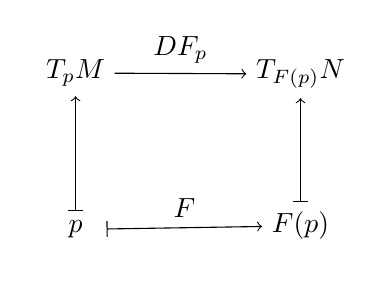
\begin{tikzpicture}
  \matrix (m) [matrix of math nodes, row sep=3.8em, column sep=4.8em, minimum width=2.2em]
  {
T_pM &  T_{F(p)}N \\
p &  F(p) \\
};
  \path[|->]
  (m-2-1) edge node [above] {$$} (m-1-1)
          edge node [auto]  {$F$} (m-2-2)
  (m-2-2) edge node [auto]  {$$} (m-1-2);
  \path[->]
  (m-1-1) edge node [above] {$DF_p$} (m-1-2);
\end{tikzpicture}

Let \quad \, $\begin{aligned} & \quad \\
 &  \text{dim}M = \text{dim}T_pM = m \\
 &  \text{dim}N = \text{dim}T_{F(p)}N = n 
\end{aligned}$

Now $DF_p : T_pM \to \text{im}(DF_p) \subseteq T_{F(p)}N$

Let $r = \text{rank}DF_p = \text{dim}\text{im}(DF_p)$.  

$r\leq n$ (clearly, since $\text{im}(DF_p) \subseteq T_{F(p)}N$)

Recall nullity-rank theorem: For linear $T: V \to T(V) = \text{im}T$, \\
\phantom{Recall} $\text{dim}\text{im}T + \text{ker}T = \text{dim}V$ \\
\phantom{Recall} $\Longrightarrow \text{dim}\text{im}T = \text{dim}V - \text{ker}T \leq \text{dim}V$.  \\
$\Longrightarrow r \leq m$

\begin{definition}
        For smooth $F: M \to N$ \\
        \textbf{smooth submersion} $F$ if $dF$ surjective $\Longleftrightarrow  \text{rank}DF_p = \text{dim} T_{F(p)}N$ i.e. $r=n$ \\
        \textbf{smooth immersion} $F$ if $dF$ injective $\Longleftrightarrow  \text{rank}DF_p = \text{dim} T_{p}M$ i.e. $r=m$ \\
\end{definition}

\exercisehead{4.4} cf. \url{http://www.math.ucla.edu/~iacoley/hw/diffhwfall/HW%202.pdf} For $q=F(p)$,

If $DF_p$, $DG_q$ surjective, $DG_q\circ DF_p = D(G\circ F)_p$ surjective.  $G\circ F$ smooth submersion.  \\
If $DF_p$, $DG_q$ injective, $DG_q\circ DF_p = D(G\circ F)_p$ injective.  $G\circ F$ smooth immersion.   \\

It'd be instructive to view this as a commutative diagram.  For 

$\begin{aligned} & \quad \\ 
                 & F: M \to N \\        
                 & G : N \to P \\
                 & p \in M \\
                 & q = F(p) \in N \\
                 & G(q) \in P \end{aligned}$ 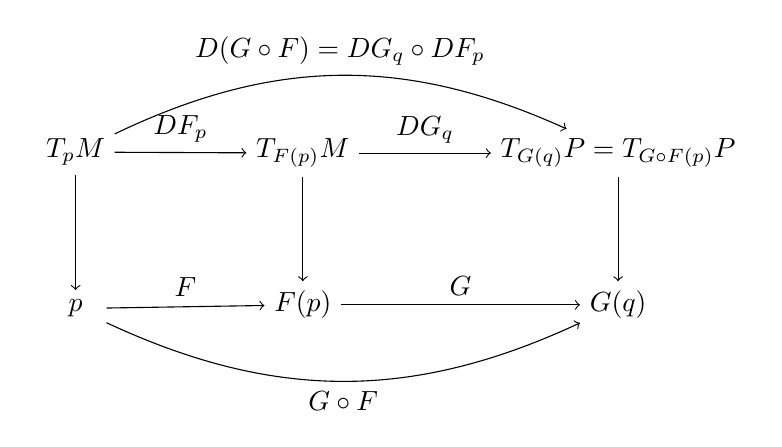
\begin{tikzpicture}
  \matrix (m) [matrix of math nodes, row sep=3.8em, column sep=4.8em, minimum width=2.2em]
  {
T_pM & T_{F(p)}M  &  T_{G(q)}P = T_{G\circ F(p)}P \\
p & F(p) & G(q) \\ 
};
  \path[->]
  (m-1-1) edge node [above] {$DF_p$} (m-1-2)
  edge[bend left=25] node [above] {$D(G\circ F) = DG_q\circ DF_p$} (m-1-3)
  edge node [auto] {$$} (m-2-1)
  (m-1-2) edge node [above] {$DG_q$} (m-1-3)
  edge node [auto] {$$} (m-2-2)
  (m-1-3) edge node [auto] {$$} (m-2-3)
  (m-2-1) edge node [above] {$F$} (m-2-2)
  edge[bend right=25] node [below] {$G\circ F$} (m-2-3)
  (m-2-2) edge node [above] {$G$} (m-2-3)  
;
\end{tikzpicture} 




\subsection*{ The Inverse Function Theorem and Its Friends }

\begin{theorem}[7.6] (\textbf{Inverse Function Theorem}). Suppose open $U,V \subset \mathbb{R}^n$, smooth $F: U \to V$ \\
If $DF(p)$ nonsingular, $p \in U$, $\exists \, $ connected neighborhood $\begin{aligned} & \quad \\ & U_0 \subset U \ni p \\ & V_0 \subset V \ni F(p) \end{aligned}$

s.t. $\left. F \right|_{U_0} : U_0 \to V_0$ diffeomorphism.  
\end{theorem}

Let $X$ metric space.  $G:X \to X$ contraction if $\exists \, \lambda <1$ s.t. $d(G(x), G(y)) \leq \lambda d(x,y)$, \, $\forall \, x, y \in X$.  \\
Clearly, $\forall \, $ contraction is cont.  

\begin{lemma}[7.7] (Contraction Lemma)
Let $X$ complete metric space \\
$\forall \,$ contraction $G: X \to X$, \, $\exists \, !$ fixed pt., i.e. $x\in X$ s.t. $G(x) = x$
\end{lemma}

\begin{theorem}[7.9] (Implicit Function Theorem)
  Let open $U \subset \mathbb{R}^n \times \mathbb{R}^k$, $(x,y) = (x^1 \dots x^n, y^1 \dots y^k)$ coordinates on $U$.  \\

Suppose $\Phi : U \to \mathbb{R}^k$ smooth.  $(a,b) \in U$, $c = \Phi(a,b)$

If $k\times k$ matrix 
\[
\frac{ \partial \Phi^i }{ \partial y^j }(a,b)
\]
nonsingular, \\
then $\exists \, $ neighborhoods $\begin{aligned} & \quad \\ 
  & V_0 \subset \mathbb{R}^n \\ 
  & W_0 \subset \mathbb{R}^k \end{aligned}$,  \\
smooth $F: V_0 \to W_0$ s.t. \\
$(\Phi^{-1}(c) ) V_0 \times W_0$ is the graph of $F$, i.e. $\Phi(x,y) = c$, $\forall \, (x,y) \in V_0 \times W_0$ iff $y= F(x)$


\end{theorem}



\subsection*{Embeddings}

\begin{definition}
\textbf{smooth embedding} of $M$ into $N$, $F$, if \\
\phantom{ \quad \, } smooth immersion $F: M\to N$ and \\
\phantom{ \quad \quad \, } $F$ topological embedding i.e. $F$ homeomorphism onto its image $F(M) \subseteq N$ in subspace topology.  

\end{definition}

\exercisehead{4.16}

Let $\begin{aligned} & \quad \\
    & F : M \to N \\
    & G:N \to P \end{aligned}$.  \\
$F,G$ smooth immersions so $G\circ F$ smooth immersion (cf. Exercise 4.4, idea is composition of $DF, DG$ is injective).  \\
Now $(G \circ F)(M) = G(F(M))$ \\
$F,G$ bijective onto $F(M)$, $G(N)$.  $G$ bijective on $F(M) \subseteq N$ onto $G(F(M))$.  Then $G\circ F$ bijective on $M$ onto $G(F(M))$ \\
$F,G$ cont., so $G\circ F $ cont.  \\
$F^{-1},G^{-1}$ cont., so $(G\circ F)^{-1}= F^{-1} \circ G^{-1}$ cont.  \\
$G\circ F$ homeomorphism onto $G\circ F(M) \subseteq P$.  

So $G\circ F$ is a smooth embedding.  


\begin{proposition}[4.22]
        Suppose smooth manifolds $M,N$, with or without boundaries, and \\
injective smooth immersion $F:M\to N$

If any of the following holds, then $F$ is a smooth embedding. 
\begin{enumerate}
        \item[(a)] $F$ open or closed map
        \item[(b)] $F$ proper map
        \item[(c)] $M$ compact
        \item[(d)] $M$ has empty boundary and $\text{dim}M = \text{dim}N$
\end{enumerate}
\end{proposition}


\section{Submanifolds}

\subsubsection*{Examples of Embedded Submanifolds }

\begin{lemma}[8.6] (\textbf{Graphs as Submanifolds}). 
If open $U \subset \mathbb{R}^n$, smooth $F: U \to \mathbb{R}^k$, \\
then graph of $F$ is an embedded $n$-dim. submanifold of $\mathbb{R}^{n+k}$
\end{lemma}

\begin{proof}
  Define $\begin{aligned} 
    & \quad \\
    & \varphi: U \times \mathbb{R}^k \to U \times \mathbb{R}^k \\ 
    & \varphi(x,y) = (x,y - F(x)) \end{aligned}$

$\varphi$ clearly smooth. \\
$\varphi$ diffeomorphism because its inverse can be written explicitly
\[
\varphi^{-1}(u,v) = (u ,  v + F(u))
\]

$\varphi( \Gamma(F))$ is the slice $\lbrace (u,v) : v = 0 \rbrace $ of $U\times \mathbb{R}^k$, so graph $\Gamma(F)$ is an embedded submanifold.  



\end{proof}



\subsubsection*{Level Sets}


\subsection*{Immersed Submanifolds}

\begin{definition}
  \textbf{immersed submanifold } of $M$, $S$, is $S\subseteq M$, with topology (not necessarily subspace topology) with respect to which it's a topological manifold (without boundary), and \\
\phantom{ \quad \quad \, }   smooth structure with respect to inclusion map $i : S \hookrightarrow M$ is smooth immersion (recall $Di \equiv i_*$ injective $\Longleftrightarrow \text{rank}Di = \text{dim}S$ \\

$\text{codim}S = \text{dim}M - \text{dim}S$ \\

\textbf{smooth hypersurface} is immersed submanifold of codimension $1$.  
\end{definition}




\section{The Cotangent Bundle}


\subsection*{ Covectors }

$V$ finite-dim. vector space

\emph{covector} on $V$ - real-valued linear functional on $V$, i.e. linear map $\omega : V\to \mathbb{R}$



\exercisehead{6.1} Suppose $\sum a_i \epsilon^i = A = 0$.  Consider arbitrary $v= v^i e_i$.  $A(v) = \sum a_i \epsilon^i (v^j e_j) = \sum a_i v^i = 0 $

$v$ arbitrary so let $v = \delta_k^{\, \, j} e_j$.  $\forall \, i, \, a_i =0$.  linearly independent.  

Consider linear map $\omega: V \to \mathbb{R}$, a covector.  
\[
\begin{gathered}
  \omega (v^i e_i ) = v^i(\omega( e_i)) = k \in \mathbb{R} \\
  \omega(e_i) = \omega_j \delta^j_{\, \, i} = \omega_j \epsilon^j( e_i)
\end{gathered}
\]
So $\omega$ spanned by $\omega_j \epsilon^j$.  Done.  



\exercisehead{6.2} $X \in V$ 

\[
\begin{gathered}
  (A^* \omega)(aX + bY) = \omega(A (aX + bY)) = a\omega(AX) + b \omega(AY) \in \mathbb{R} \text{ since } \omega: W^* \to \mathbb{R}
\end{gathered}
\]
linear map $A^* \omega :V \to \mathbb{R}$ is a functional.

\[
A^*(a\omega + b\nu)(X) = (a\omega + b\nu )(AX) = a\omega(AX)+ b \nu(AX) \in \mathbb{R}
\]

\exercisehead{6.3}

\begin{enumerate}
\item[(a)] 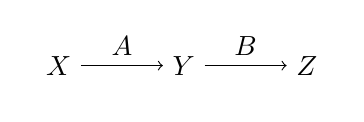
\begin{tikzpicture}
  \matrix (m) [matrix of math nodes, row sep=2em, column sep=3em, minimum width=1em]
  {
    X  & Y & Z  \\ };
  \path[->]
  (m-1-1) edge node [auto] {$A$} (m-1-2)
  (m-1-2) edge node [auto] { $B$} (m-1-3);
%  (m-2-1) edge node [below] {$\widetilde{A}$} (m-1-2);
\end{tikzpicture}

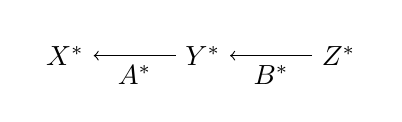
\begin{tikzpicture}
  \matrix (m) [matrix of math nodes, row sep=2em, column sep=3em, minimum width=1em]
  {
    X^*  & Y^* & Z^*  \\ };
  \path[->]
  (m-1-2) edge node [auto] {$A^*$} (m-1-1)
  (m-1-3) edge node [auto] { $B^*$} (m-1-2);
%  (m-2-1) edge node [below] {$\widetilde{A}$} (m-1-2);
\end{tikzpicture}


$(BA)^* : Z^* \to X^*$
\[
((BA)^* \zeta)(x) = \zeta(BAx) = (\zeta B)(Ax) = (B^* \zeta)(Ax) = (A^* B^*)\zeta(x)
\]

\item[(b)]
\[
(Id_V)^*(\nu(x)) = \nu(1x) = \nu(x)
\]
\end{enumerate}

\subsection*{ Tangent Covectors on Manifolds}



\subsection*{ The Cotangent Bundle}

\begin{proposition}[6.5] Let $M$ smooth manifold, $T^*M = \coprod_{p \in M} T_p^*M$ \\
with $\begin{aligned} & \quad \\ 
  & \pi : T^*M \to M \\ 
  & \omega \in T^*_pM \to p \end{aligned}$

natural vector space structure on each fiber, \\
$\exists \, !$ smooth manifold structure making $T*M$ rank-$n$ vector bundle over $M$, \\
s.t. all coordinate covectors are smooth local sections
\end{proposition}

\subsection*{ The Differential of a Function }



\section{Lie Groups}

% file: 07LieGroups.tex
% 07LieGroups Chapter 7 Lie Groups of Introduction to Smooth Manifolds J. Lee, latest edition (as of 20150331)
% Typeset with LaTeX format
% cf. Math Into Latex Third Edition pp. 290
% This file has my modifications
% Fund Science! & Help Ernest in Physics Research! : quantum super-A-polynomials - researched by Ernest Yeung \\
% http://igg.me/at/ernestyalumni2014 
% Facebook      : ernestyalumni 
% github        : ernestyalumni
% gmail         : ernestyalumni 
% linkedin      : ernestyalumni 
% tumblr        : ernestyalumni 
% twitter       : ernestyalumni 
% wordpress.com : ernestyalumni
% youtube       : ernestyalumni 
% Patreon       : ernestyalumni
% Tilt/Open     : ernestyalumni
%
% Ernest Yeung was supported by Mr. and Mrs. C.W. Yeung, Prof. Robert A. Rosenstone, Michael Drown, Arvid Kingl, Mr. and Mrs. Valerie Cheng, and the Foundation for Polish Sciences, Warsaw University.
% 
% This code is open-source, governed by the Creative Common license.  Use of this code is governed by the Caltech Honor Code: ``No member of the Caltech community shall take unfair advantage of any other member of the Caltech community.'' 
% 

\subsection*{Basic Definitions}

\textbf{Lie group} smooth manifold $G$ s.t. multiplication map $\begin{aligned} & \quad \\ 
  & m : G \times G \to G \\
  & m(g,h) = gh \end{aligned}$ \\
inversion map $\begin{aligned} & \quad \\ 
  & i : G \to G \\
  & i(g) = g^{-1} \end{aligned}$ 
smooth.

\begin{proposition}[7.1]
If $(g,h) \mapsto gh^{-1}$ smooth, $G$ Lie group
\end{proposition}
\exercisehead{7.2}
\begin{proof}
  $\forall \, g,h \in G$, $gh^2 \in G$ since $G$ group \\
$(gh^2,h) \mapsto gh$ smooth.  Define $m(g,h) = (gh^2,h) \mapsto gh$.  So $m$ smooth.  \\
$1\in G$ since $G$ group.  $(1,g) \mapsto g^{-1}$ smooth so $i(g) = g^{-1}$, defined this way, smooth.  
\end{proof}

\textbf{Example 7.3 (Lie Groups)}.  
\begin{enumerate}
\item[(a)]$A \in GL(n,\mathbb{R})$
\[
\begin{aligned}
  & (AB)_{ij} = A_{ik} B_{kj} \quad \quad \, \begin{aligned} & \quad \\ 
    & \frac{ \partial (AB)_{ij} }{ \partial A_{lm} } = \delta_{il} \delta_{km} B_{kj} = \delta_{il} B_{mj} \\ 
    & \frac{ \partial (AB)_{ij} }{ \partial B_{lm} } = A_{ik} \delta_{lk} \delta_{mj} = A_{il} \delta_{mj} \end{aligned} \\
  & (A^{-1})_{ij} = \frac{1}{ \text{det}(A)} \text{adj}(A)_{ij} = \frac{1}{ \text{det}(A) } C^T_{ij} = \frac{1}{ \text{det}(A)}(-1)^{i+j}\text{det}A_{ji}
\end{aligned}
\]
$AB,A^{-1}$ smooth functions of the entires of $A_{ij}$, $B_{kl}$, $A_{ij}$ respectively.
\item[(b)]
\item[(c)]
\end{enumerate}

\subsection*{Lie Group Homomorphisms}

\textbf{Example 7.4 (Lie Group Homomorphisms)}

\begin{enumerate}
\item[(a)]
\item[(b)]
\item[(c)]
\item[(d)]
\item[(e)]
\item[(f)] \textbf{conjugation} by $g$
\[
\begin{aligned}
  & C_g : G \to G \\ 
  & C_g(h) = ghg^{-1}
\end{aligned}
\]
$H \subseteq G$ \textbf{normal} if $C_g(H) = H$, \, $\forall \, g \in G$
\end{enumerate}

\begin{theorem}[7.5]
  Every Lie group homomorphism has constant rank.
\end{theorem}





\section{Vector Fields}

% 08VectorFields.tex
% Fund Science! & Help Ernest finish his Physics Research! : quantum super-A-polynomials - a thesis by Ernest Yeung
%                                               
% http://igg.me/at/ernestyalumni2014                                                                             
%                                                              
% Facebook     : ernestyalumni  
% github       : ernestyalumni                                                                     
% gmail        : ernestyalumni                                                                     
% google       : ernestyalumni                                                                                   
% linkedin     : ernestyalumni                                                                             
% tumblr       : ernestyalumni                                                               
% twitter      : ernestyalumni                                                             
% youtube      : ernestyalumni                                                                
% indiegogo    : ernestyalumni                                                                        
%
% Ernest Yeung was supported by Mr. and Mrs. C.W. Yeung, Prof. Robert A. Rosenstone, Michael Drown, Arvid Kingl, Mr. and Mrs. Valerie Cheng, and the Foundation for Polish Sciences, Warsaw University.                  
% 
% Caltech Honor Code and the spirit of Open Source/Creative Commons 
%




\exercisehead{4.1} 
Consider $ \begin{aligned} & \quad \\ 
  & 1 : \mathbb{R}^n \to \mathbb{R}^n \\ & x^i(x) = x^i \end{aligned}$, \quad \, smooth structure on $\mathbb{R}^n$, that's open.  

Consider $\begin{aligned} & \quad \\ 
  & F: T\mathbb{R}^n \to \mathbb{R}^{2n} \\
& F(x^1 \dots x^n, v^1 \dots v^n ) = (x^1 \dots x^n, v^1 \dots v^n) \end{aligned}$ \\
$F= F^{-1}$, so clearly $F = 1_{T\mathbb{R}^n} $ is cont., bijective, and it's inverse cont. and smooth.  $F$ diffeomorphism.  

\exercisehead{4.2}  $F:M \to N$.  Consider (3.6)

\[
\begin{gathered}
  \begin{aligned}
    & (U , \varphi) \subset M \quad \quad \, \varphi = (x^1 \dots x^m) \\ 
    & (V, \psi ) \subset N \quad \quad \, \psi = (y^1 \dots y^n) 
\end{aligned}  \quad \quad \quad \, \begin{aligned} & X = X^i \frac{ \partial }{ \partial x^i } \\ 
    & Y = Y^j \frac{ \partial }{ \partial y^j } \end{aligned}
\end{gathered}
\]

\[
(F_* X)(f) = Y^j \frac{ \partial }{ \partial y^j} f = X(fF) = X^i \frac{ \partial }{ \partial x^i } fF = X^i \frac{ \partial (f\psi^{-1})}{ \partial y^j} \frac{ \partial }{ \partial x^i } (\psi F^j \varphi^{-1})(\varphi(p)) = X^i \frac{ \partial F^j}{ \partial x^i }(p) \frac{ \partial f}{ \partial y^j}
\]
where
\[
fF = f\psi^{-1} \psi F\varphi^{-1} \varphi \Longrightarrow fF(p) = (f\psi^{-1})(y) (\psi F\varphi^{-1})(\varphi(p))
\]
(a serious case of abuse of notation)

For $F_*X$, 
\[
Y^j = X^i \frac{ \partial F^j}{ \partial x^i}
\]

\[
F_* \left. \frac{ \partial }{ \partial x^i } \right|_p = F_* \frac{ \partial }{ \partial x^i} = \delta_i^{ \, \, k } \frac{ \partial F^j}{ \partial x^k} \frac{ \partial }{ \partial y^j} = \frac{ \partial F^j}{ \partial x^i } \frac{ \partial }{ \partial y^j} = \frac{ \partial F^j}{ \partial x^i}(p) \left. \frac{ \partial }{ \partial y^j } \right|_{F(p)}
\]
with $X^k = \delta_i^{\, \, k}$

\[
\begin{aligned}
  &  F_* : TM \to TN \\
  & F_*( x^1 \dots x^n, v^1 \dots v^n) = (y^1(x) \dots y^n(x), v^i \frac{ \partial F^1}{ \partial x^i} \dots v^i \frac{ \partial F^n}{ \partial x^i} )
\end{aligned}
\]
Clearly $F_*$ smooth since $F$ smooth.  

\begin{lemma}[4.8] Suppose smooth $F: M \to N$, \, $\begin{aligned} & \quad \\ & Y \in \tau(M) \\ & Z \in \tau(N) \end{aligned}$ \\
$Y,Z$, $F$-related iff $\forall \, $ smooth $\mathbb{R}$-valued $f$ on open $V \subset N$, 
\[
Y(fF) = (Zf) F \quad \quad \quad (4.4) 
\]
\end{lemma}

\begin{proof}
  $\forall \, p \in M$, $\forall \, $ smooth $\mathbb{R}$-valued $f$, $f$ defined near $F(p)$
\[
\begin{gathered}
  Y(fF)(p) = Y_p(fF) = (F_* Y_p)f \quad \quad \quad (F_*Y)f = Y(fF) \\ 
  (Zf)F(p) = (Zf)(F(p)) = Z_{F(p)}f  
\end{gathered}
\]
if $(Zf) F(p) = Y(fF)(p) = Zf = (F_*Y) f $ 
\[
(Zf)F = Y(fF) \Longleftrightarrow Z = F_* Y \text{ i.e. iff $Y, Z$ \, $F$-related }
\] 

\end{proof}



\subsubsection*{ Vector Fields on a Manifold with Boundary}

\subsection*{ Lie Brackets }

\begin{lemma}[4.12] Lie bracket of smooth vector fields $V,W$, $\begin{aligned} & \quad \\
    & [V, W ] : C^{\infty} M \to C^{\infty} M \\ 
    & [V, W ] f = VW f - WV f \end{aligned}$ \quad is a smooth vector fields.  
\end{lemma}

\begin{proof}
  By Prop. 4.7.  ($M$ smooth, map $\mathcal{Y} : C^{\infty}M \to C^{\infty} M$ is a derivation iff $\mathcal{Y} f = Yf$, $Y$ some smooth vector field $Y \in \tau(M)$.  \\
Suffices to show $[V,W]$ derivation of $C^{\infty}M$  
\[
\begin{gathered}
  [V,W] (fg) = V(W(fg)) -  W(V(fg)) = V(fWg + gWf) - W( fVg  + gVf) = \\
   = VfWg + fVW g + Vg Wf + gVWf - WfVg - fWVg - WgVf - gWVf  = \\
   =fVWg + gVWf - fWV g - gWVf = f[V,W] g + g[V,W]f
\end{gathered}
\]
\end{proof}


extremely useful coordinate formula for Lie bracket 
\begin{lemma}[4.13]
  Let $\begin{aligned} & \quad \\
    & V = V^i \frac{ \partial }{ \partial x^i} \\ 
    & W = W^j \frac{ \partial }{ \partial x^j} \end{aligned}$ \quad \quad $\begin{aligned}
    & [V,W] = \left( V^i \frac{ \partial W^j}{ \partial x^i } - W^i \frac{ \partial V^j}{ \partial x^i } \right) \frac{ \partial }{ \partial x^j } \quad \quad \quad (45) \\ 
    & [V,W]  = (VW^j - WV^j) \frac{\partial }{ \partial x^j} \quad \quad \quad (46) \end{aligned}$

\end{lemma}

\begin{proof}
  $[V,W]$ smooth vector field already, its values are determined locally $\left. ([V,W] f ) \right|_U = [V,W] ( \left. f \right|_U )$  \\
It suffices to compute in a single smooth chart.  
\[
\begin{gathered}
[V,W] f = V^i \frac{ \partial }{ \partial x^i } \left( W^j \frac{ \partial f}{ \partial x^j} \right) - W^j \frac{ \partial }{ \partial x^j} \left( V^i \frac{ \partial f}{ \partial x^i }\right) = V^i \frac{ \partial W^i}{ \partial x^i } \frac{ \partial f}{ \partial x^j} + V^i W^j \frac{ \partial^2 f}{ \partial x^i \partial x^j } - W^j \frac{ \partial V^i }{ \partial x^j} \frac{ \partial f}{ \partial x^i } - W^j V^i \frac{ \partial^2 f}{ \partial x^j  \partial x^i } = \\
= \left( V^i \frac{ \partial W^j}{ \partial x^i } - W^i \frac{ \partial V^j}{ \partial x^i} \right) \frac{ \partial f}{ \partial x^j}
\end{gathered}
\]

\end{proof}

\exercisehead{4.6}

For Lemma 4.15 (Properties of the Lie Bracket), part (d), 

the point is to use the derivative properties of the vector fields.  

\[
\begin{gathered}
  \left[fV, gW \right] h = fV( gW h ) - gW (fVh) = (fVg)(Wh) + g(fV(Wh)) - (gWf)(Vh) - f(gW)(Vh) = \\
  = g( f VW) h - (fgWV)h +   f(Vg)W h - g(Wf)Vh
\end{gathered}
\]

\begin{proposition}[4.16] (Naturality of the Lie Bracket)
  Let smooth $F:M \to N$, \quad $\begin{aligned} & \quad \\ & V_1, V_2 \in \tau(M) \\ & W_1, W_2 \in \tau(N) \end{aligned}$, \quad $V_i$ \, $F$-related to $W_i$, $i=1,2$.  

Then $[V_1, V_2 ]$ $F$-related to $[W_1, W_2]$

\end{proposition}

\begin{proof}
Use Lemma 4.8, and given $V_i$, \, $F$-related to $W_i$  

\[
\begin{aligned}
  & V_1 V_2 (fF) = V_1 (W_2 f) F = W_1 W_2 fF \\ 
  & V_2 V_1 (fF) = (W_2 W_1 f) F
\end{aligned} \quad \quad \Longrightarrow [V_1, V_2](fF) = ( [W_1, W_2] f)F
\]
So $[V_1, V_2]$ , \, $F$-related to $[W_1, W_2]$
\end{proof}

\begin{corollary}[4.17]
  Suppose $F: M \to N$ diffeomorphism, $V_1, V_2 \in \tau(M)$ \\
Then $F_*[V_1, V_2] = [F_* V_1, F_* V_2 ]$

\end{corollary}

\begin{proof} $F$ diffeomorphism.  Then Lemma 4.9, $\exists \, $ push-forward (or alternatively, by Prop. 4.16, $W_i = F_* V_i$ i.e. $F$-related).  
\[
F_*[V_1, V_2 ] = [W_1, W_2 ] =  [F_* V_1, F_*V_2]
\]
\end{proof}

\subsection*{ The Lie Algebra of a Lie Group }

\[
L_g = m i_g 
\]

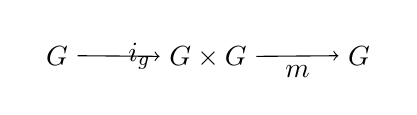
\begin{tikzpicture}
  \matrix (m) [matrix of math nodes, row sep=2em, column sep=3em, minimum width=1em]
  {
%    U_i \subset \mathbb{R}^{n+1} - 0 &  \\
%    V_i \subset \mathbb{R}P^n  & \mathbb{R}^n  \\ };
G & G \times G & G   \\  };
%  \path[-stealth]
  \path[->]
  (m-1-1) edge node [right] {$i_g$} (m-1-2)
  (m-1-2) edge node [below] {$m$} (m-1-3);
\end{tikzpicture}

$i_g(h) = (g,h)$, $m$ is multiplication, follows $L_g$ smooth.  

$L_g$ diffeomorphism of $G$, since $L_{g^{-1}}$ smooth inverse. 

$\forall \, $ 2 pts. $g_1, g_2 \in G$, \, $\exists \, ! \, L_{g_2 g_1^{-1}}$ s.t. $L_{g_2 g_1^{-1}} g_1 = g_2$  many important properties of Lie groups follow from $L_{g_2 g_1^{-1}}$ as diffeomorphism.  

vector field $X$ on $G$ \emph{left invariant} if 
\begin{equation}
  (L_g)_* X_{g'} = X_{gg'} \quad \quad \forall \, g, g' \in G \quad \quad \quad (4.8)
\end{equation}

$L_g$ diffeomorphism.  
\[
(L_g)_*(aX+ bY) = a(L_g)_*X + b(L_g)_* Y
\]
set of all smooth left-invariant vector fields on $G$ is a linear subspace $\tau(M)$, \emph{ and } closed under Lie bracket.  

\begin{lemma}[4.18] 
Let $G$ Lie group, suppose $X,Y$ smooth left-invariant vector fields on $G$ \\
Then $[X,Y]$ also left invariant.  
\end{lemma}

\begin{proof}
  Given $\begin{aligned} & \quad \\ & (L_g)_*X = X \\ & (L_g)_* Y = Y \end{aligned}$ by def. of left-invariance.  
\end{proof}









\subsection*{Vector Fields on Manifolds}

\begin{lemma}[8.6] \textbf{(Extension Lemma for Vector Fields)} \\
  $M$ smooth manifold with or without boundary \\
$A \subseteq M$ closed subset. \\
Suppose $X$ smooth vector field along $A$.  \\
Give open $U \supset A$, $\exists \, $ smooth global vector field $\widetilde{X}$ on $M$ s.t. $\left. \widetilde{X} \right|_A = X$ and $\text{supp}{\widetilde{X}} \subseteq U$
\end{lemma}

\exercisehead{8.9}

\begin{enumerate}
\item[(a)] $\forall \, p \in M$, \, $\begin{aligned} & \quad \\
  & X_p = X^i(p) \frac{ \partial }{ \partial x^i} \\
  & Y_p = Y^i(p) \frac{ \partial }{ \partial x^i } \end{aligned}$ \\
$f,g \in C^{\infty}{(M)}$

\[
\begin{aligned}
  & (fX)_p = f(p)X_p = f(p) X^i(p) \frac{ \partial }{ \partial x^i } \\ 
  & (gY)_p = g(p)Y_p = g(p)Y^i(p) \frac{ \partial }{ \partial x^i }
\end{aligned}
\]
\[
(fX + gY)_p  = f(p)X_p + g(p)Y_p = f(p) X^i(p) \frac{ \partial}{ \partial x^i} + g(p)Y^i(p) \frac{ \partial }{ \partial x^i } = (f(p)X^i(p) + g(p) Y^i(p)) \frac{ \partial }{ \partial x^i }
\]
$f(p)X^i(p) + g(p)Y^i(p)$ smooth so $(fX+gY)_p$ smooth.
\item[(b)] Let $g=f$ 
\[
(fX+fY)_p = f(p)X_p + f(p)Y_p = f(p)X^i(p) \frac{ \partial }{ \partial x^i} + f(p)Y^i(p)\frac{ \partial}{\partial x^i} = f(p)(X^i(p) + Y^i(p))\frac{ \partial }{ \partial x^i } = (f(X+Y))_p
\]
Let $Y=X$ so $\forall \, p$, 
\[
(fX+gX)_p  = f(p)X_p + g(p)X_p = f(p)X^i(p)\frac{ \partial}{ \partial x^i} +g(p)X^i(p) \frac{ \partial }{ \partial x^i} = (f(p) + g(p))X^i(p)\frac{ \partial }{ \partial x^i } = ((f+g)X)_p
\]

\[
(g(fX))_p = g(p)(fX)_p= g(p)f(p)X_p = ((gf)X)_p
\]
Let $f=1$, $g=0$, $1X=X$
\end{enumerate}





\hrulefill

\subsubsection*{Local and Global Frames}

\subsubsection*{Vector Fields as Derivations of $C^{\infty}(M)$}

if $X \in \mathfrak{X}(M)$, smooth $f$ defined on open $U\subseteq M$, obtain
\[
\begin{aligned}
  & Xf : U \to \mathbb{R} \\  
  & (Xf)(p) = X_p F
\end{aligned}
\]
From J. Lee: (Be careful not to confuse the notations $fX$ and $Xf$: the former is the smooth \emph{vector field} on $U$ obtained by multiplying $X$ by $f$, while the latter is the real-valued \emph{function} on $U$ obtained by applying the vector field $X$ to the smooth function $f$)

\begin{proposition}[8.14]
$X: M \to TM$ 

equivalent
\begin{enumerate}
\item[(a)] $X$ smooth 
\item[(b)] $\forall \, f \in C^{\infty}(M)$, $Xf $ smooth on $M$ 
\item[(c)] $\forall \, $ open $U \subseteq M$, $\forall \, f \in C^{\infty}(M)$, $Xf \in C^{\infty}(U)$
\end{enumerate}
\end{proposition}

\begin{proof}
  (a) $\Longrightarrow $ (b), assume $X$ smooth, \\
let $f\in C^{\infty}(M)$ \\
$M$ manifold, $\forall \, p \in M$, choose smooth $x^i$ on open $U\ni p$ \\
Then $\forall \, x \in U$, 
\[
Xf(x) = \left( \left. X^i(x) \frac{ \partial }{ \partial x^i} \right|_x \right) f = X^i(x) \frac{ \partial f}{ \partial x^i}(x)
\]
$X^i$ smooth on $U$ by Prop. 8.1, $Xf$ smooth in $U$
\end{proof}

\subsection*{Vector Fields and Smooth Maps}

\begin{proposition}[8.16]
  Suppose smooth $F:M\to N$, \quad \, $\begin{aligned} & \quad \\ 
    & X \in \mathfrak{X}(M) \\
    & Y \in \mathfrak{X}(N) \end{aligned}$ \\

Then $X,Y$ $F$-related iff $\forall \, $ smooth $h$, defined on open $V \subset N$ 
\[
X(hF) = (Yh)F
\]



\end{proposition}

\begin{proof}
$\forall \, p \in M$, $\forall \, $ smooth $h$ defined on open $V \ni F(p)$ 
\[
\begin{aligned}
  & X(hF)(p) = X_p(hF) = dF_p(X_p)h \\ 
  & (Yh)F(p) = Yh(F(p)) = Y_{F(p)}h
\end{aligned}
\]
$X(hF) = (Yh)F$ \quad \, $\forall \, h \in C^{\infty}(N)$ iff $dF_p(X_p) = Y_{F(p)}$ \, $\forall \, p$




\end{proof}




\begin{proposition}[8.19]
  smooth $M,N$, diffeomorphism $F:M \to N$ \\
$\forall \, X \in \mathfrak{X}(M)$, $\exists \, !$ smooth vector field on $N$ $F$-related to $X$
\end{proposition}

\begin{proof}
$\forall \, p \in M$, $F(p) = q\in N$  \\

define $Y$ by 
\[
\begin{aligned}
  & Y_q = dF_{F^{-1}(q)}(X_{F^{-1}(q)} ) = dF_p(X_p) \\ 
  \Longrightarrow & Y_{F(p)} = dF_p(X_p) 
\end{aligned}
\]
$Y: N \to TN$ 
\[
Y = N \xrightarrow{F^{-1}} M \xrightarrow{X} TM \xrightarrow{dF} TN
\]
$Y = dF \circ X \circ F^{-1}$

$dF, X, F^{-1}$ smooth.  $Y$ smooth. 
\end{proof}
\textbf{pushforward} of $X$ by $F$, denote $F_*X$ 
\begin{equation}
  (F_*X)_q = dF_{F^{-1}(q)}(X_{F^{-1}(q) } ) \quad \quad \quad \, (8.7)
\end{equation}
$(F_*X)_q = dF_p(X_p)$



\begin{corollary}[8.21]
  Suppose diffeomorphism $F: M \to N$, $X \in \mathfrak{X}(M)$ \\
  $\forall \, h \in C^{\infty}(N)$
\[
((F_*X)h) \circ F = X(h\circ F)
\]
\end{corollary}


\subsubsection*{Vector Fields and Submanifolds}


\subsection*{Lie Brackets}

\begin{proposition}[8.26] \textbf{(Coordinate Formula for the Lie Bracket)}
  \begin{equation}
    [X,Y] = \left( X^i \frac{ \partial Y^j}{ \partial x^i } - Y^i \frac{ \partial X^j}{ \partial x^i } \right) \frac{\partial}{ \partial x^j }  \quad \quad \quad \, (8.8)
\end{equation}
\end{proposition}

\subsection*{The Lie Algebra of a Lie Group}

Recall that $G$ acts smoothly and transitively on itself by left translation:
\[
L_g(h) = gh
\]

$X$ on $G$ \textbf{left-invariant} if 
\begin{equation}
d(L_g)_{g'}(X_{g'}) = X_{gg'} \quad \, \forall \, g, g' \in G \quad \quad \quad \, (8.12)
\end{equation}

$L_g$ diffeomorphism, so 
\[
(L_g)_*X = X \quad \quad \, \forall \, g \in G
\]





\textbf{Example 8.36 (Lie Algebras)}

\begin{enumerate}
\item[(a)]
\item[(b)]
\item[(c)]
\item[(d)]
\item[(e)]
\item[(f)] $\forall \, $ vector $V$ becomes Lie algebra if $[,]=0$ \\
such a Lie algebra is \textbf{abelian}
\end{enumerate}

$\text{Lie}{G}$ Lie algebra of all smooth left-invariant vector fields on Lie Group $G$ \textbf{ Lie algebra of $G$ }



\begin{theorem}[8.37] $\begin{aligned}  & \quad \\
    & \epsilon : \text{Lie}{(G)} \to T_eG \\ 
    & \epsilon(X) = X_e \end{aligned}$

$\epsilon$ vector space isomorphism
\end{theorem}

\begin{proof}
  If $\epsilon(X) = X_e = 0$ for some $X \in \text{Lie}{(G)}$

left invariant $d(L_g)_{g'}(X_{g'}) = X_{gg'}$
\[
d(L_g)_e(X_e) = X_g=0 \quad \, \forall \, g \in G, \text{ so } X= 0 
\]
$\epsilon$ injective

Let $V \in T_eG$ arbitrary. \\
\quad define (rough) vector field $v^L$ on $G$ by 
\begin{equation}
  \left. v^L \right|_g = d(L_g)_e(v) \quad \quad \quad \, (8.13)
\end{equation}

\end{proof}





\textbf{Example 8.40}
\begin{enumerate}
\item[(a)] $L_b(x) = b + x$  \quad \quad \, $bx = b + x$ \quad \quad \, $y = x + b$ \\

$d(L_g) = 1$ \\
$X_x = X^i \frac{ \partial }{ \partial x^i }$ \\
$d(L_b)_x X_x = 1 X_x = X_x = \widetilde{X}^i \frac{ \partial }{ \partial (x+b)} = \widetilde{X}^i(x+b) \frac{ \partial }{ \partial x} = X^i(x) \frac{ \partial }{ \partial x^i }$

$X^i$ constants \\

$[X,Y]=0$ if $X,Y$ constants. 

lie algebra of $\mathbb{R}^n$ abelian (cf. Example 8.36, (f))
\item[(b)]
\item[(c)]
\end{enumerate}

\begin{proposition}[8.41] \textbf{(Lie Algebra of the General Linear Group)}
  \begin{equation}
    \text{Lie}{(GL(n,\mathbb{R}))} \to T_{1_n}GL(n,\mathbb{R}) \to \mathfrak{gl}{(n,\mathbb{R})} \quad \quad \, (8.14)
\end{equation}
is isomorphism
\end{proposition}

\begin{proof}
global coordinates $X^i_{ \, \, j}$ on $GL(n,\mathbb{R})$

natural isomorphism
\[
\begin{gathered}
  T_1GL(n,\mathbb{R}) \longleftrightarrow \mathfrak{gl}(n,\mathbb{R}) \\
  A^i_{ \, \, j } \left. \frac{ \partial }{ \partial X^i_{ \, \, j }} \right|_{1_n} \longleftrightarrow (A^i_{ \, \, j})
\end{gathered}
\]


Recall 
\[
d(L_g)_{g'}(X_{g'}) = X_{gg'}
\]
Recall Lie algebra of all smooth left invariant vector fields on $G$ \\ 
Recall (8.13)
\begin{equation}
\left. v \right|_g = d(L_g)_e(v) \quad \quad \quad \, (8.13)
\end{equation}

$L_X$ is restriction to $GL(n,\mathbb{R})$ of linear map $A \mapsto XA$ on $\mathfrak{gl}{(n,\mathbb{R})}$  

\[
\begin{aligned}
  & L_X g = Xg = X^i_{ \, \, k } g^k_{ \, \, j } \\ 
  & L_X 1 = X1 = X^i_{ \, \, k } \delta^k_{ \, \, j } = X^i_{ \, \, j } = X
\end{aligned}
\]

$X^i_{ \, \, j}$ global coordinates on $GL(n,\mathbb{R})$, so
\[
\left. \frac{ \partial }{ \partial X^i_{\, \, j}} \right|_1 = \left. \frac{ \partial }{ \partial X^i_{\, \, j}} \right|_X
\]

\[
DL_X = \frac{ \partial}{ \partial A^k_{ \, \, j} } ( XA)^i_{ \, \, j} = \frac{ \partial }{ \partial A^k_{ \, \, l} } X^i_{ \, \, m} A^m_{ \, \, j} = X^i_{ \, \, m} \delta^m_{ \, \, k } \delta^l_{ \, \, j } = X^i_{ \, \, k } \delta^i_{ \, \, j}
\]

\[
(DL_X)_1(A) = ((DL_X)^{i \, \, \, l }_{ \, \, j \, \, \, k } A^k_{\, \, l} \left. \frac{ \partial }{ \partial X^i_{ \, \, j } } \right|_X = ( X^i_{ \, \, k } \delta^l_{ \, \, j} A^k_{ \, \, l } ) \left. \frac{ \partial }{ \partial X^i_{ \, \, j } }\right|_X = (X^i_{ \, \, k} A^k_{ \, \, j} ) \left. \frac{ \partial }{ \partial X^i_{ \, \, j} } \right|_X
\]


\end{proof}




\subsection*{Problems}

\problemhead{8-1}

$\forall \, p \in A$, choose neighborhood $W_p$ of $p$, smooth $\widetilde{X}:A \to TM$ s.t. $\widetilde{X} = X$ on $W_p \bigcap A$

Replace $W_p$ by $W_p \bigcap U$, so $W_p \subseteq U$

$\lbrace W_p | p \in A \rbrace \bigcup \lbrace M \backslash A \rbrace$ open cover of $M$

Let $\lbrace \psi_p | p \in A \rbrace \bigcup \lbrace \psi_0 \rbrace$ smooth partition of unity subordinate to this cover, with $\text{supp}{\psi_p} \subseteq W_p$, $\text{supp}{\psi_0} \subseteq M \backslash A$

$\forall \, p \in A$, $(U_p,x^i)$ smooth coordinate chart

\[
\begin{gathered}
  X_p = \left. X^i(p) \frac{ \partial }{ \partial x^i } \right|_p \\ 
  X^i: U_p \to \mathbb{R}
\end{gathered}
\]

$\psi_p \widetilde{X}^i(p)$ smooth on $W_p$

$\psi_p\widetilde{X}^i(p)$ has smooth extension to all of $M$ if $\psi_p \widetilde{X}^i(p) =0$ on $M\backslash \text{supp}{\psi_p}$ \\

on open $W_p \backslash \text{supp}{ \psi_p}$, they agree

define $\widetilde{X}^i:M \to \mathbb{R}$ 
\[
\widetilde{X}^i(x) = \sum_{p \in A} \psi_p(x) \widetilde{X}^i(p)
\]

$\lbrace \text{supp}{\psi_p} \rbrace$ locally finite, so $\sum_{p\in A} \psi_p(x) \widetilde{X}^i(p)$ has only finite number of nonzero terms in neighborhood of $\forall \, x \in M$, so $\widetilde{X}^i(x)$ smooth

If $x\in A$, $\psi_0(x) = 0$, $\widetilde{X}^i(x) = X^i(x)$ \quad \, $\forall \, p $ s.t. $\psi_p(x) \neq 0$, so 
\[
\widetilde{X}^i(x) = \sum_{p\in A} \psi_p(x) X^i(x) = (\psi_0(x) + \sum_{p\in A} \psi_p(x)) X^i(x) = X^i(x)
\]
so $\widetilde{X}^i$ extension of $X$


\hrulefill

\problemhead{8-2} \textsc{Euler's Homogeneous Function Theorem} 
$y = \lambda x$
\[
\frac{ \partial f}{ \partial y^i } \frac{ \partial y^i}{ \partial \lambda} = x^i \frac{ \partial f}{ \partial y^i} = x^i \frac{ \partial f}{ \partial ( \lambda x^i)} = \frac{d}{d\lambda} f(y) = \frac{d}{d\lambda} f(\lambda x) = \frac{d}{d\lambda} ( \lambda^c f(x)) = c \lambda^{c-1} f(x)
\]

$\lambda = 1$

\[
\boxed{ x^i \frac{ \partial f}{ \partial x^i } = V_x f(x) = cf(x) }
\]


\hrulefill




\problemhead{8-29}

\[
\begin{aligned}
  & \mathfrak{o}{(n)} = \lbrace A \in \mathfrak{gl}(n,\mathbb{R}) | A^T + A = 0 \rbrace \\ 
  & \mathfrak{o}{(3)} = \lbrace A \in \mathfrak{gl}(3,\mathbb{R}) | A^T + A = 0 \rbrace 
\end{aligned}
\]


\[
\begin{aligned}
& \mathfrak{su}(n) = \lbrace A \in \mathfrak{gl}(n,\mathbb{C}) | A^* + A = 0 , \text{tr}A = 0 \brace \\ 
& \mathfrak{su}(2) = \lbrace A \in \mathfrak{gl}(2,\mathbb{C}) | A^* + A = 0 , \text{tr}A = 0 \brace \\ 
\end{aligned}
\]

$\forall \, A \in \mathfrak{su}(2)$, $A$ is of the form, for $a,b,c \in \mathbb{R}$, 
\[
A = \left( \begin{matrix} ia & b + ic \\ 
  -b + i c & -ia \end{matrix} \right)
\]
$\forall \, B \in \mathfrak{o}(3)$, $B$ is of the form 
\[
B = \left( \begin{matrix}  & a & b \\ 
  -a & & c \\ 
  -b & -c & \end{matrix} \right)
\]
Then the following identification, $F$ is clearly an isomorphism, as its 1-to-1 and onto:
\[
\begin{aligned}
  & F : \mathfrak{su}(2) \to \mathfrak{o}(3) \\ 
  & F\left( \begin{matrix} ia & b + ic \\ 
    -b + ic & -ia \end{matrix} \right) = \left( \begin{matrix} & a & b \\ 
    -a & & c \\
    -b & -c & \end{matrix} \right)
\end{aligned}
\]



\section{Integral Curves and Flows }



\subsection*{Integral Curves }

If smooth curve $ \begin{aligned} & \quad \\ 
 c:  & I \to M \\  
 c(t) & = p \end{aligned}$ \\
$\forall \, t \in I ,  \, c' \equiv c'(t) \in T_{c(t)}M \equiv T_p M$ \\

If $X$ vector field on $M$, \\
integral curve of $X$ is differentiable $c: I  \to M$ s.t. \\
\quad $\forall \, t \in I$, $c'(t) \equiv \dot{c} = X_{c(t)} = X_p$  \\

EY  \\
\[
\begin{aligned}
  & c:I \to M \\ 
  & c(t) = p  \\
  & \varphi c(t) = \varphi(p) \Longrightarrow \begin{aligned} & c^i(t) = x^i(t) \\
    & \dot{c}^i(t) = \dot{x}^i(t) \end{aligned} \\
  X_p = X^i(p) \frac{ \partial }{ \partial x^i } \equiv X^i \frac{ \partial }{ \partial x^i } = \dot{c}^i \frac{ \partial }{ \partial x^i } 
\end{aligned}
\]

\[
\begin{gathered}
  f: M \to \mathbb{R} \\ 
  X_p f = X_p f(p) = X_pf \varphi^{-1} \varphi(p) = X_(f\varphi^{-1})(x^j) = X^i \frac{ \partial f}{ \partial x^i }(x^j) \equiv X^i(p)  \frac{ \partial f}{ \partial x^i}(x^j) = \dot{c}^i \left. \frac{ \partial f}{ \partial x^i} \right|_p = \frac{d}{dt}( f \circ c)(t)
\end{gathered}
\]




Example 9.1.  (Integral Curves)

\begin{enumerate}
\item[(a)] Let $X = \frac{ \partial }{ \partial x}$, $(x,y) \in \mathbb{R}^2$ 

\[
\begin{gathered}
  c(t) = (x(t), y(t)) = x \partial_x + y\partial_y \\ 
  c' = \dot{x} \partial_x + \dot{y} \partial_y = \partial_y   \Longrightarrow \dot{y} = 0 \quad \, y = b \\
  \dot{x} = 1 \quad \quad \, x = a+t \\ 
  c = (a+t ,b) 
\end{gathered}
\]


\item[(b)] $X = x\partial_x - y \partial_x$.  Comparing the components of these vectors, we see that this is equivalent to 

\[
\begin{gathered}
  \begin{aligned}
    \dot{x} & = -y \\
    \dot{y}  & = x \end{aligned} \Longrightarrow \begin{aligned}
    y & = a \sin{t} + b\cos{t} \\ 
    x & = a\cos{t} - b\sin{t} \end{aligned}
\end{gathered}
\]



\end{enumerate}


\begin{proposition}[9.2] Let smooth vector field $X$ on smooth $M$, \\
$\forall \, p \in M$, $\exists \, \epsilon > 0 $, $\exists \, $ smooth $c:(-\epsilon, \epsilon) \to M$ i.e. integral curve of $X$ starting at $p$ \end{proposition}

\begin{proof}
  existence from Thm. D.1
\end{proof}


\begin{lemma}[9.3] (Rescaling Lemma) 
$\widetilde{ c}(t) = c(at)$ integral curve of $aX$, where $\widetilde{I} = \lbrace t | at \in I \rbrace$
\end{lemma}
\begin{proof} Let smooth $f$ defined in neighborhood of $\widetilde{c}(t_0)$ \\
e.g. of rescaling  - $2t = 2\cdot 1 = 2 \quad \, a=2$ 

\[
\begin{gathered}
  \widetilde{c}(t) = c(at) = c(\tau) = p \in M \\ 
  \dot{ \widetilde{c}}(t) f = \frac{d}{dt} (f\circ \widetilde{c})(t) = \frac{d}{dt} (f\varphi^{-1})( \varphi\widetilde{c}(t)) = \frac{d}{dt} (f\varphi^{-1})(\varphi c(at) ) = \frac{d}{dt} (f\varphi^{-1})(c^i(at)) = \left. \frac{ \partial f}{ \partial x^i} \right|_p \frac{dc^i}{ d\tau}(\tau)a = a \frac{d}{d \tau}(f\circ c)(\tau) = aX_p f
\end{gathered}
\]


\end{proof}

\begin{lemma}[9.4] (Translation Lemma)
\[
\begin{aligned}
  & \widetilde{I} = \lbrace t | t + a \in I \rbrace \\ 
  & \widetilde{c}(t) = c(t+a)
\end{aligned}
\]



\end{lemma}

\exercisehead{9.5}
\begin{proof}
\[  
\begin{aligned}
&  \widetilde{c}(t) = c(t+a) = c(\tau) = p \in M \\ 
&  \dot{ \widetilde{c}}(t) f = \frac{d}{dt} (f\circ \widetilde{c})(t) = \frac{d}{dt} f(\widetilde{c}(t)) = \frac{d}{dt} f(c(t+a) ) = \left. \frac{ \partial f}{ \partial x^i } \right|_p \frac{d c^i(\tau) }{ d\tau } = \dot{c}^i(\tau)  \left. \frac{ \partial f}{ \partial x^i } \right|_p = X^i_p \left. \frac{ \partial f}{ \partial x^i} \right|_p = X_p f
\end{aligned}
\]
\end{proof}




\begin{proposition}[9.6] (Naturality of Integral curves)
  Suppose smooth $F: M \to N$ \\
  \quad Then $\begin{aligned} & \quad \\ 
    & X \in \mathfrak{X}(M) \\
    & Y \in \mathfrak{X}(N) \end{aligned}$ \quad \, $F$-related iff $F$ takes integral curves of $X$ to integral curves of $Y$
\end{proposition}

\begin{proof}
Recall 
\[
X,Y \, F-\text{related means } \, dF(X) =Y
\]

Let $\gamma = Fc$ 
\[
\dot{\gamma} = \frac{d}{dt} (F\circ c)(t) = (dF)(\dot{c}) = dF(X) = Y
\]

$\Longrightarrow \gamma $ integral curve of $Y$ \\

if $\gamma = Fc$ integral curve of $Y$, $\dot{\gamma} = Y$.  \quad $q = F(p)$.  $p=c(t)$

\[
\begin{gathered}
  Yg= Y_qg = Y^j \left. \frac{ \partial g}{ \partial y^j } \right|_q = \dot{\gamma}^j(t) \left. \frac{ \partial g}{ \partial y^j } \right|_{F(p)} = \frac{d}{dt} (F\circ c ) \left. \frac{ \partial g}{ \partial y^j } \right|_{F(p)} = \frac{ \partial y^j}{ \partial x^k } \dot{c}^k(t) \left. \frac{ \partial g}{ \partial y^j } \right|_q = \frac{ \partial y^j}{ \partial x^k} X^k_p \left. \frac{ \partial g}{ \partial y^j } \right|_q = (F_* X)g = dF(X)g \\
\Longrightarrow dF(X) = Y
\end{gathered}
\]
\end{proof}


\subsection*{Flows }


Let $X \in \mathfrak{X}(M)$ \\
Suppose $\forall \, p \in M$, $\exists \, !$ \, integral curve starting at $p$, $\phi^{(p)}: \mathbb{R} \to M$ \\
$\forall \, t \in \mathbb{R}$, define $\begin{aligned} & \quad \\
  & \phi_t: M \to M \\
  & \phi_t(p) = \phi^{(p)}(t) \end{aligned}$

\[
\theta_0(p) = \theta^{(p)}(0) = p
\]

EY: $\phi_t$ pushes $p$ to $\phi^{(p)}(t)$ over time interval $t$ \\

translation lemma implies $t\mapsto \phi^{(p)}(t+s)$ is integral curve of $X$ starting at $q = \phi^{(p)}(s)$  \\

assuming uniqueness of integral curves, $\phi^{(p)}(t) = \phi^{(p)}(t+s)$, so 

\[
\begin{gathered}
  \phi_t \circ \phi_s(p) = \phi_{t+s}(p) \\ 
  \phi_0(p) = \phi^{(p)}(0) = p 
\end{gathered}
\]

$\Longrightarrow \phi : \mathbb{R}\times M \to M$ is an action of additive group $\mathbb{R}$ on $M$.  \\

define \emph{ global flow } on $M$ (1-parameter group action) - cont. left $\mathbb{R}$-action on $M$, i.e. \\
\quad cont. $\phi : \mathbb{R} \times M \to M$ s.t. $\forall \, s,t \in \mathbb{R}$, $\forall \, p M$ 

\begin{equation}
\begin{aligned}
& \phi(t, \phi(s,p) ) = \phi(t+s, p )
& \phi(0,p) = p 
\end{aligned} \quad \quad \quad \, (9.2)
\end{equation}

given global flow $\phi$ \\

$\forall \, t \in \mathbb{R}$, define cont. $\begin{aligned} & \quad \\
  & \phi_t: M \to M \\
  & \phi_t(p) \to \phi(t,p)
\end{aligned}$  
\[
\xrightarrow{ (9.2) } \begin{gathered}
  \phi_t \cdot \phi_s = \phi_{t+s} \\ 
  \phi_0 = 1_M
\end{gathered}
\]

$\phi_t : M \to M$ homeomorphism; if flow smooth, $\phi_t$ diffeomorphism.   \\

$\forall \, p \in M$, define $ \begin{aligned} & \quad \\ & \phi^{(p)}:\mathbb{R} \to M \\ & \phi^{(p)}(t) = \phi(t,p) \end{aligned}$ \\

$\phi^{(p)}$ is orbit of $p$ under group action.  

smooth global flow $\theta:\mathbb{R} \times M \to M$ \\
\quad $\forall \, p \in M$, define $V_p \in T_pM$
\[
V_p = (\theta^{(p)})'(0)
\]


\begin{proposition}[9.7] Let smooth global flow $\phi: \mathbb{R}\times M \to M$ on smooth $M$ \\
infinitesimal generator $X$ of $\phi$ \quad $\begin{aligned} & \quad \\
  & p \mapsto X_p \\
  & X_p  = \dot{\phi}^{(p)}(0) \end{aligned}$ \quad is smooth vector field on $M$, and $\forall \, \phi^{(p)}$, $\phi^{(p)}$ integral curve of $X$ 
\end{proposition}

\begin{proof}
  Show $X$ smooth.  Use Prop. 8.14,  \\
$f$ smooth on open $U\subseteq M$, $f:U\to \mathbb{R}$ 

\[
Xf(p) = X_pf = \dot{\phi}^{(p)}(0) f \equiv ( \dot{\phi}^{(p)}(0) )[f] = \left. \frac{d}{dt} ( f\circ \phi^{(p)} ) \right|_{t=0} = \frac{ \partial }{ \partial t} \left. (f\circ \phi(t,p) ) \right|_{t=0} 
\]

$f\circ \phi(t,p) = f(\phi(t,p))$ smooth function of $(t,p)$ by composition, so $\partial_t(f\circ \phi)$ smooth. So $Xf$ smooth, so $X$ smooth.   \\

Let $q = \phi^{(p)}(a) = \phi_a(p)$ 

\begin{equation}
  \phi^{(q)}(t) = \phi_t(q) = \phi_t( \phi_a(p)) = \phi_{t+a}(p) = \phi^{(p)}(t+a) \quad \quad \quad \, (9.4)
\end{equation}

\begin{equation}
  X_qf = \dot{\phi}^{(q)}(0)f = \dot{\phi}^{(q)}(0)[f] = \frac{d}{dt} \left. (f \circ \phi^{(q)}(t)) \right|_{t=0} = \frac{d}{dt} \left. (f\circ \phi^{(p)}(t+a) ) \right|_{t=0} = \dot{\phi}^{(p)}(a) f = X_{ \phi^{(p)}(a) } f \quad \quad \quad \, (9.5)
\end{equation}

\end{proof}

So by def., $\phi^{(p)}(t)$ integral curve of $X$


\subsubsection*{ The Fundamental Theorem on Flows }

flow domain for $M$ is open $\mathcal{D} \subseteq \mathbb{R} \times M$ s.t. $\forall \, p \in M$, $\mathcal{D}^{(p)} = \lbrace t \in \mathbb{R} | (t,p) \in \mathcal{D} \rbrace$ is an open interval containing $0$.  \\

\textbf{flow} on $M$ is cont. $\phi : \mathcal{D} \to M$ s.t. group laws : 
\begin{equation}
  \forall \, p \in M, \, \phi(0, p ) = p \quad \quad \quad \, (9.6)
\end{equation}

\begin{equation}
  \begin{aligned} & \quad \\ 
    & \forall \, s \in \mathcal{D}^{(p)} \\ 
    & \forall \, t \in \mathcal{D}^{ (\phi(s,p))} \end{aligned} \quad \text{ s.t. } s + t \in \mathcal{D}^{(p)}, \quad \quad \, \phi(t, \phi(s,p) ) = \phi(t+s, p ) \quad \quad \quad \, (9.7)
\end{equation}

\begin{proposition}[9.11] If $\phi: \mathcal{D} \to M$ smooth flow, \\
then infinitesimal generator $X$ of $\phi$ smooth vector field and $\forall \, \phi^{(p)}$ integral curve of $X$
\end{proposition}

\begin{proof}
Recall that  \\
\emph{infinitesimal generator} $X$ of $\phi$, $\begin{aligned} & \quad \\ 
  & p \mapsto X_p \\
  & X_p = \dot{\phi}(0) \end{aligned}$ \quad now on open $\mathcal{D}$, $\mathcal{D} \subseteq \mathbb{R} \times M$ s.t. $\forall \, p \in M$, $\mathcal{D}^{(p)} = \lbrace t \in \mathbb{R} | (t,p) \in \mathcal{D} \rbrace$ open, \\

given $\phi$ smooth flow, \\
\quad $\phi(t,q)$ defined and smooth $\forall \, (t,q)$ sufficiently close to $(0,p)$ since $\mathcal{D}$ open.  With $f$ smooth on open $U$ in this open neighborhood of $(0,p)$, 

\[
\Longrightarrow Xf(p) = \left. \frac{ \partial }{ \partial t } (f \circ \phi(t,p)) \right|_{t=0}
\]

$f\phi$ smooth (by composition), so $\partial_t f\phi$ smooth, so $X$ smooth itself around $\forall \, p \in M$.   \\

Suppose $t\in \mathcal{D}^{(p)}$ \\
$\mathcal{D}^{(p)}$, $\mathcal{D}^{ (\phi_t(p))} = \mathcal{D}^{(q)}$ open (by def.)

$\phi_{\Delta t}\phi_t(p) = \phi_{ \Delta t + t }(p)$ by def. of flow. 









\end{proof}

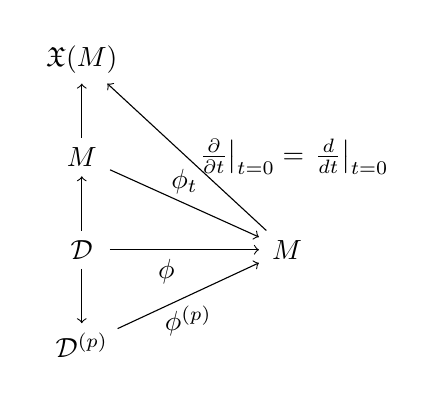
\begin{tikzpicture}
  \matrix (m) [matrix of math nodes, row sep=2em, column sep=4.8em, minimum width=2em]
  {
\mathfrak{X}(M) &  \\
M &  \\
\mathcal{D} &       M \\
\mathcal{D}^{(p)} & \\
};
  \path[->]
  (m-2-1) edge node [above] {$$} (m-1-1)
  edge node [above] {$\phi_t$} (m-3-2)
  (m-3-1) edge node [auto] {$$} (m-2-1)
  edge node [below left] {$\phi$} (m-3-2)
  edge node [auto] {$$} (m-4-1)
  (m-4-1) edge node [below] {$\phi^{(p)}$} (m-3-2)
  (m-3-2) edge node [right] {$\left. \frac{ \partial }{ \partial t} \right|_{t=0} = \left. \frac{d}{dt} \right|_{t=0}$} (m-1-1)
;
\end{tikzpicture} \quad \quad \quad \, 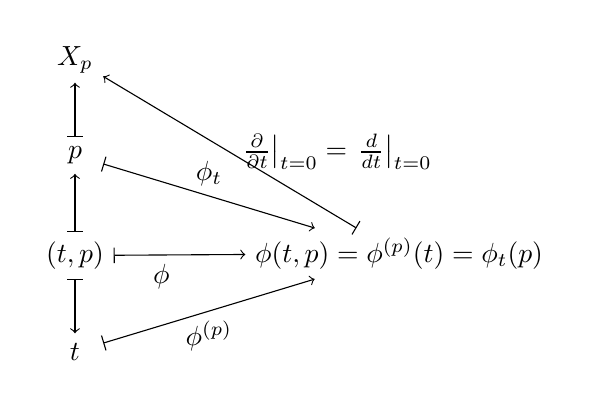
\begin{tikzpicture}
  \matrix (m) [matrix of math nodes, row sep=2em, column sep=4.8em, minimum width=2em]
  {
X_p &  \\
p &  \\
(t,p)       &       \phi(t,p) = \phi^{(p)}(t) = \phi_t(p) \\
t & \\
};
  \path[|->]
  (m-2-1) edge node [above] {$$} (m-1-1)
  edge node [above] {$\phi_t$} (m-3-2)
  (m-3-1) edge node [auto] {$$} (m-2-1)
  edge node [below left] {$\phi$} (m-3-2)
  edge node [auto] {$$} (m-4-1)
  (m-4-1) edge node [below] {$\phi^{(p)}$} (m-3-2)
  (m-3-2) edge node [right] {$\left. \frac{ \partial }{ \partial t} \right|_{t=0} = \left. \frac{d}{dt} \right|_{t=0}$} (m-1-1)
;
\end{tikzpicture}





\begin{theorem}[9.12] (Fundamental Theorem on Flows)
  Let smooth vector field $X$ on smooth manifold $M$.  \\
$\exists \, ! \, \, $ smooth maximal flow $\phi : \mathcal{D} \to M$ whose infinitesimal generator is $X$ (recall $\begin{aligned} & \quad \\ 
    & p \mapsto X_p \\
    & X_p = \dot{\phi}{(0)} \end{aligned}$) s.t. 
\begin{enumerate}
\item[(a)] $\forall \, p \in M$, curve $\phi^{(p)} : \mathcal{D}^{(p)} \to M$ is unique maximal integral curve of $X$ starting at $p$. 
\item[(b)] If $s\in \mathcal{D}^{(p)}$, then $\mathcal{D}^{(\phi(s,p))}$ is interval $\mathcal{D}^{(p)}-s = \lbrace t - s | t\in \mathcal{D}^{(p)} \rbrace$
\item[(c)] $\forall \, t \in \mathbb{R}$, $M_t$ open in $M$, and $\phi_t:M_t \to M_{-t}$ diffeomorphism with inverse $\phi_{-t}$
\end{enumerate}
\end{theorem}

\begin{proof}
From Proposition 9.2 ($\forall \, p \in M$, $\exists \, \epsilon > 0$, \, $\exists \, $ smooth $c:(-\epsilon, \epsilon) \to M$, i.e. integral curve $X$ starting at $p$) \\

Suppose $c,\widetilde{c} : I \to M$ \, 2 integral curves of $X$, open $I$ s.t. $c(t_0) = \widetilde{c}(t_0)$ for some $t_0 \in I$ \\
Let $S = \lbrace t | t \in I, \text{ s.t. } c(t) = \widetilde{c}(t) \rbrace$ \\
Clearly $S \neq \emptyset$ since $c(t_0) = \widetilde{c}(t_0)$ \quad (hypothesis) \\
\quad $S$ closed in $I$ by continuity (of $c, \widetilde{c}$) \\
Suppose $t_1 \in S$ \\
\quad $c(t_1) = \widetilde{c}(t_1)=p$
Then in smooth coordinate neighborhood around $p=c(t_1)$, \, $c, \widetilde{c}$ both solutions to same ODE with same initial conditions $c(t_1) = \widetilde{c}(t_1) = p$ \\

By uniqueness part of Thm. D.1, $c\equiv \widetilde{c}$ on interval containing $t_1$ \\
\quad $\Longrightarrow S $ \, open in $I$. \\
Since $I$ connected, $S=I$ \quad ($S$ clopen) \\
$c= \widetilde{c} \quad \, \forall \, t \in I$ \\
Thus, $\forall \, c , \widetilde{c}$ \, that agrees at 1 pt. agree on common domain.   \\ 

$\forall \, p \in M$, let $\mathcal{D}^{(p)} = \bigcup_{\alpha} I_{\alpha}$, open $I_{\alpha} \subseteq \mathbb{R}$ 
\quad s.t. $0 \in I_{\alpha}$, and integral curve $\begin{aligned} & \quad \\ 
  & c_{\alpha} : I_{\alpha} \to M \\
  & c_{\alpha}(0) = p \end{aligned}$ \, starting at $p$ is defined.  \\

define $\begin{aligned} & \quad \\ 
  & \phi^{(p)}: \mathcal{D}^{(p)} \to M  \\
  & \phi^{(p)}(t) = c(t) \end{aligned}$ \, where $c$ is any integral curve s.t. $c(0) = p$ and $c$ defined on $I_{\alpha}$ s.t. $0,t \in I_{\alpha}$. \\

since all integral curves agree at $t$ by argument above, $\phi^{(p)}$ well-defined \\
\quad \quad and is obviously unique maximal integral curve starting at $p$.   \\


Let $\mathcal{D} = \lbrace (t,p) \in \mathbb{R} \times M | t \in \mathcal{D}^{(p)} \rbrace$ \\
define $\begin{aligned} & \quad \\ 
  & \phi :\mathcal{D} \to M \\
  & \phi{(t,p)} = \phi^{(p)}{(t)} \equiv \phi_t{(p)} \end{aligned}$ (notation for last statement)  \\

By def. $\phi$ satisfies (a): $\forall \, p \in M$, $\exists \, ! \, $ maximal integral curve of $X$, $\phi^{(p)}$, starting at $p$.  \\

Fix $p\in M$, $s \in \mathcal{D}^{(p)}$ \\
write $q = \phi{ (s,p) } = \phi^{(p)}(s)$ \\

define $\begin{aligned} & \quad \\ 
  & \widetilde{c}: \mathcal{D}^{(p)} -s \to M \\
  & \widetilde{c}(t) = \phi^{(p)}(t+s) \, \text{ s.t. } \, \widetilde{c}{(0)} = \phi^{(p)}(s) = q \end{aligned}$ \\

By translation lemma (9.4), $\begin{aligned} & \quad \\
  & \widetilde{c}{(t)} = c{(t+s)} \\
  & \widetilde{I} = \lbrace t | t+s \in I \rbrace \end{aligned}$ \quad \, e.g. $\begin{aligned} & \quad \\ 
  & I = (-2,6) , \, \, s = 1 \\
  & \widetilde{I} = (-3,5) \end{aligned}$ \quad \, $\widetilde{c}(t)$ also integral curve of $X$.  

By uniqueness of ODE solutions, \\
\quad $\widetilde{c}$ agrees with $\phi^{(q)}$ on their common domain, \\
\quad \quad equivalent to second group law (9.7) 
\[
\widetilde{c}{(t)} = \phi^{(p)}{ (t+s)} = \phi{(t+s,p)} = \phi^{(q)}{(t)} = \phi{(t,q)} = \phi{(t,\phi{(s,p) }) }
\]



\end{proof}


\begin{lemma}[9.19] \textbf{(Escape Lemma)}
Suppose smooth $M$, $V\in \mathfrak{X}(M)$.  \\
If $\gamma: J \to M$ maximal integral curve of $V$ s.t. domain $J$ has finite least upper bound $b$, \\
\phantom{ \quad \, } then $\forall \, t_0 \in J$, $\gamma([t_0,b))$ not contained in any compact subset of $M$
\end{lemma}

\begin{proof}
See Problem 9-6.  Solution there.  
\end{proof}

\subsection*{Flowouts}

Suppose smooth $M$, $S\subseteq M$ embedded $k$-dim. submanifold. \\
smooth $V \in \mathfrak{X}(M)$ s.t. $V$ nowhere tangent to $S$.  \\
Let $\theta:\mathcal{D} \to M$ be flow of $V$  \\
Let $\mathcal{O} = (\mathbb{R}\times S) \bigcap \mathcal{D}$ \\
\phantom{Let } $\Phi= \left. \theta \right|_{\mathcal{O}}$
\begin{enumerate}
\item[(a)] $\Phi : \mathcal{O} \to M$ immersion 
\item[(b)] $\frac{ \partial }{ \partial t} \in \mathfrak{X}(\mathcal{O})$ is $\Phi$-related to $V$
\item[(c)] $\exists \, $ smooth $\delta >0$, $\delta : S \to \mathbb{R}$ s.t. \\
$\left. \Phi \right|_{\mathcal{O}_{\delta}}$ injective, where $\mathcal{O}_{\delta} \subseteq \mathcal{O}$ flow domain.  
\begin{equation}
  \mathcal{O}_{\delta} = \lbrace (t,p) \in \mathcal{O} | |t| < \delta(p) \rbrace \quad \quad \quad \, (9.9)
\end{equation}
Thus $\Phi(\mathcal{O}_{\delta})$ immersed submanifold of $M$ containing $S$. $V$ tangent to $\Phi(\mathcal{O}_{\delta})$
\item[(d)] If $S$ codim. $1$, $\left. \Phi \right|_{\mathcal{O}_{\delta}}$ diffeomorphism onto open submanifold of $M$
\end{enumerate}

\subsection*{Flows and Flowouts on Manifolds with Boundary }

\subsection*{Lie Derivatives }

\begin{equation}
  D_vW(p) = \left. \frac{d}{dt} \right|_{t=0} W_{p+tv} = \lim_{t\to 0} \frac{ W_{p+tv} - W_p }{t} \quad \quad \quad \, (9.15)
\end{equation}

\[
D_vW(p) = D_vW^i(p) \left. \frac{ \partial }{ \partial x^i } \right|_p
\]

\textbf{Lie derivative of $W$ with respect to $V$ }

\begin{equation}
  (\mathcal{L}_VW)_p = \left. \frac{d}{dt} \right|_{t=0} d(\theta_{-t})_{\theta_t(p)}(W_{\theta_t(p)}) = \lim_{t \to 0} \frac{ d(\theta_{-t})_{\theta_t(p)}(W_{\theta_t(p)}) - W_p }{ t } \quad \quad \quad \, (9.16)
\end{equation}

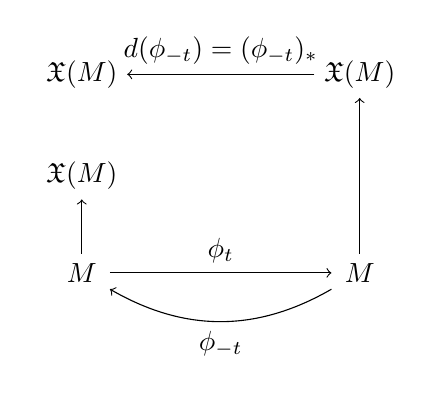
\begin{tikzpicture}
  \matrix (m) [matrix of math nodes, row sep=2em, column sep=6.8em, minimum width=2em]
  {
\mathfrak{X}(M) & \mathfrak{X}(M)  \\
\mathfrak{X}(M) &   \\
M    &       M \\
};
  \path[->]
  (m-3-1) edge node [above] {$$} (m-2-1)
  edge node [above] {$\phi_t$} (m-3-2)
  (m-3-2) edge node [auto] {$$} (m-1-2)
  edge [bend left] node [auto] {$\phi_{-t}$} (m-3-1)
  (m-1-2) edge node [above] {$d(\phi_{-t})=(\phi_{-t})_*$} (m-1-1)
;
\end{tikzpicture} \quad \quad \quad \, 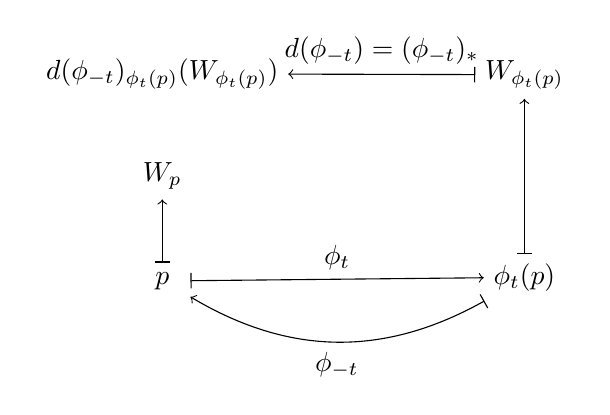
\begin{tikzpicture}
  \matrix (m) [matrix of math nodes, row sep=2em, column sep=6.8em, minimum width=2em]
  {
d(\phi_{-t})_{\phi_t(p)}(W_{\phi_t(p)}) & W_{\phi_t(p)}  \\
W_p   &    \\
p    &       \phi_t(p) \\
};
  \path[|->]
  (m-3-1) edge node [above] {$$} (m-2-1)
  edge node [above] {$\phi_t$} (m-3-2)
  (m-3-2) edge node [auto] {$$} (m-1-2)
  edge [bend left] node [auto] {$\phi_{-t}$} (m-3-1)
  (m-1-2) edge node [above] {$d(\phi_{-t})=(\phi_{-t})_*$} (m-1-1)
;
\end{tikzpicture}




\begin{lemma}[9.36]
  Suppose smooth $M$ with or without $\partial$, \, $V, W \in \mathfrak{X}(M)$ \\
If $\partial M \neq \emptyset$, assume $v$ trangent to $\partial M$ \\
Then $\exists \, $ smooth $(\mathcal{L}_VW)_p$ \, $\forall \, p \in M$
\end{lemma}

\begin{proof}
  $\forall \, (t,x ) \in J_0 \times U_0$, \\
  matrix $d(\theta_{-t})_{\theta_t(x)}: T_{\theta_t(x)}M \to T_xM$
\[
\left( \frac{ \partial \theta^i}{ \partial x^j}(-t, \theta(t,x)) \right)
\]

Therefore,
\[
d(\theta_{-t})_{\theta_t(x)}(W_{\theta_t(x)}) = \frac{ \partial \theta^i}{ \partial x^j}(-t,\theta(t,x)) W^j(\theta(t,x)) \left. \frac{ \partial }{ \partial x^i} \right|_x
\]

\end{proof}

\exercisehead{9.37}

Given $V = v^i \frac{ \partial }{ \partial x^i}$ with constant coefficients (i.e. $v^i$ constant)

\[
\begin{aligned}
  & \dot{\theta}^{(x)}(t) = V \\ 
  & \dot{\theta}^i(t) = v^i  \\
  & \theta^i(t)= v^it + x^i
\end{aligned} \quad \quad \Longrightarrow \quad 
\frac{ \partial \theta^i}{ \partial x^j} = \delta^i_{ \, \, j}
\]

\[
\begin{gathered}
\frac{d}{dt} W^i(\theta(t,x))  = \frac{ \partial W^i}{ \partial y^j}(v^j) 
\end{gathered}
\]

From the proof of Lemma 9.36, 
\[
\begin{gathered}
  d(\theta_{-t})_{\theta_t(x)}(W_{\theta_t(x)}) = \frac{ \partial \theta^i}{ \partial x^j}(-t,\theta(t,x)) W^j(\theta(t,x)) \left. \frac{ \partial }{ \partial x^i} \right|_x = \\
 = \delta^i_{ \, \, j} W^j(\theta(t,x)) \left. \frac{ \partial }{ \partial x^i} \right|_x  = W^i(\theta(t,x)) \left. \frac{ \partial }{ \partial x^i} \right|_x
\end{gathered}
\]
From (9.16)
\[
\begin{gathered}
  (\mathcal{L}_VW)_p = \left. \frac{d}{dt} \right|_{t=0} d(\theta_{-t})_{\theta_t(p)}(W_{ \theta_t(p) } ) = v^j \frac{ \partial W^i}{ \partial x^j} \left. \frac{ \partial }{ \partial x^i} \right|_p = D_VW^i(p) \left. \frac{ \partial }{ \partial x^i} \right|_p = D_VW(p)
\end{gathered}
\]

\hrulefill

\begin{theorem}[9.38] If smooth $M$, and $V,W \in \mathfrak{X}(M)$, 
\[
\mathcal{L}_VW = [V,W]
\]
\end{theorem}



\begin{corollary}[9.39]
  \begin{enumerate}
    \item[(a)]
    \item[(b)]
    \item[(c)]
    \item[(d)]
    \item[(e)]
\end{enumerate}
\end{corollary}

\exercisehead{9.40}

  \begin{enumerate}
    \item[(a)] \[
\mathcal{L}_VW = [V,W] = -[W,V] = \mathcal{L}_WV
\]
    \item[(b)]
    \item[(c)]
    \item[(d)]
    \item[(e)]
\end{enumerate}


\hrulefill


Prop. 9.41 is about derivative of $d(\theta_{-t})_{\theta_t(p)}(W_{\theta_t(p)})$ at other times

\begin{proposition}[9.41] Suppose smooth $M$ with or without $\partial$ and $V, W \in \mathfrak{X}(M)$ \\
If $\partial M \neq \emptyset$, assume $V$ tangent to $\partial M$ \\
Let $\theta$ flow of $V$.  \\

$\forall \, (t_0,p)$ in domain of $\theta$

\[
\left. \frac{d}{dt} \right|_{t=t_0} d(\theta_{-t})_{\theta_t(p)}(W_{\theta_t(p)})  = d(\theta_{-t_0}) ( (\mathcal{L}_VW)_{\theta_{t_0}(p)} )
\]
\end{proposition}


\subsection*{ Commuting Vector Fields }


\subsection*{ Time-Dependent Vector Fields }

Let smooth manifold $M$ 

\textbf{time-dependent vector field on $M$}, $V$ \\ 
\quad cont. $V: J \times M \to TM$, interval $J \subseteq \mathbb{R}$ \\
\quad \quad s.t. 
\[
V(t,p) \in T_p M \quad \, \forall \, (t,p) \in J \times M
\]
i.e. $\forall \, t \in J$, \\
$\begin{aligned}
  & V_t : M \to TM \\
  & V_t(p) = V(t,p) \end{aligned}$ is a vector field on $M$

EY : 20150226

\textbf{time-dependent vector field on $M$}, $V$ is \\
\phantom{ \quad \quad \, }  $\begin{aligned}
& \quad \\
 \text{ cont. } & V : J \times M \to TM \quad \, \text{ interval } J \subseteq \mathbb{R} \\
  & V(t,p) \in T_p M \quad \, \forall \, (t,p) \in J \times M \end{aligned}$

i.e.  $\forall \, t \in J$ \\
$\begin{aligned}
& \quad \\
  & V_t : M \to TM \\
  & V_t(p) = V(t,p ) \in \mathfrak{X}(M) \end{aligned}$


\textbf{integral curve of $V$ } is diff. $\begin{aligned} 
& \quad \\
  & \gamma : J_0 \to M \\
  & \dot{\gamma}(t) = V(t,\gamma(t)) \quad \, \forall \, t \in J_0 \end{aligned}$ \quad \, where $J_0 \subset J $ s.t. 

$\forall \, X \in \mathfrak{X}(M)$, determines time dependent vector field $V: \mathbb{R} \times M \to TM$ by 
\[
V(t,p) = X_p
\]

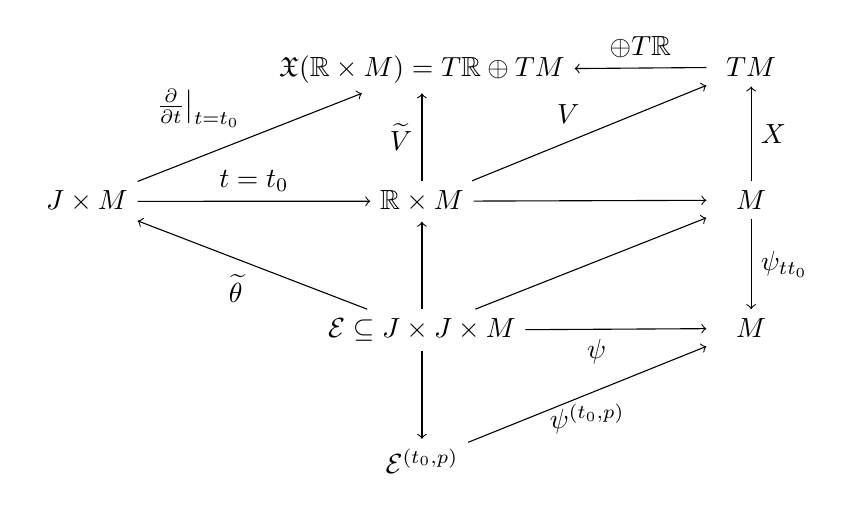
\begin{tikzpicture}
  \matrix (m) [matrix of math nodes, row sep=3.2em, column sep=4.8em, minimum width=3.2em]
  {
& \mathfrak{X}(\mathbb{R}\times M) = T\mathbb{R}\oplus TM     & TM   \\
J \times M & \mathbb{R} \times M &  M\\
& \mathcal{E} \subseteq J \times J \times M         &       M \\
& \mathcal{E}^{(t_0,p)}                            & \\
};
  \path[->]
  (m-2-2) edge node [left] {$\widetilde{V}$} (m-1-2)
         edge node [auto] {$V$} (m-1-3)
          edge node [above] {$$} (m-2-3)
  (m-3-2) edge node [auto] {$$} (m-2-2)
          edge node [auto] {$$} (m-2-3)
          edge node [below left] {$\psi$} (m-3-3)
          edge node [auto] {$$} (m-4-2)
          edge node [auto] {$\widetilde{\theta}$} (m-2-1)
  (m-4-2) edge node [below] {$\psi^{(t_0,p)}$} (m-3-3)
  (m-2-3) edge node [right] {$\psi_{tt_0}$} (m-3-3)
          edge node [right] {$X$} (m-1-3)
  (m-1-3) edge node [above] {$\oplus T\mathbb{R}$} (m-1-2)
  (m-2-1) edge node [above] {$t=t_0$} (m-2-2)
          edge node [auto] {$\left. \frac{ \partial }{ \partial t} \right|_{t=t_0}$} (m-1-2)
;
\end{tikzpicture} \quad \quad \quad \, 

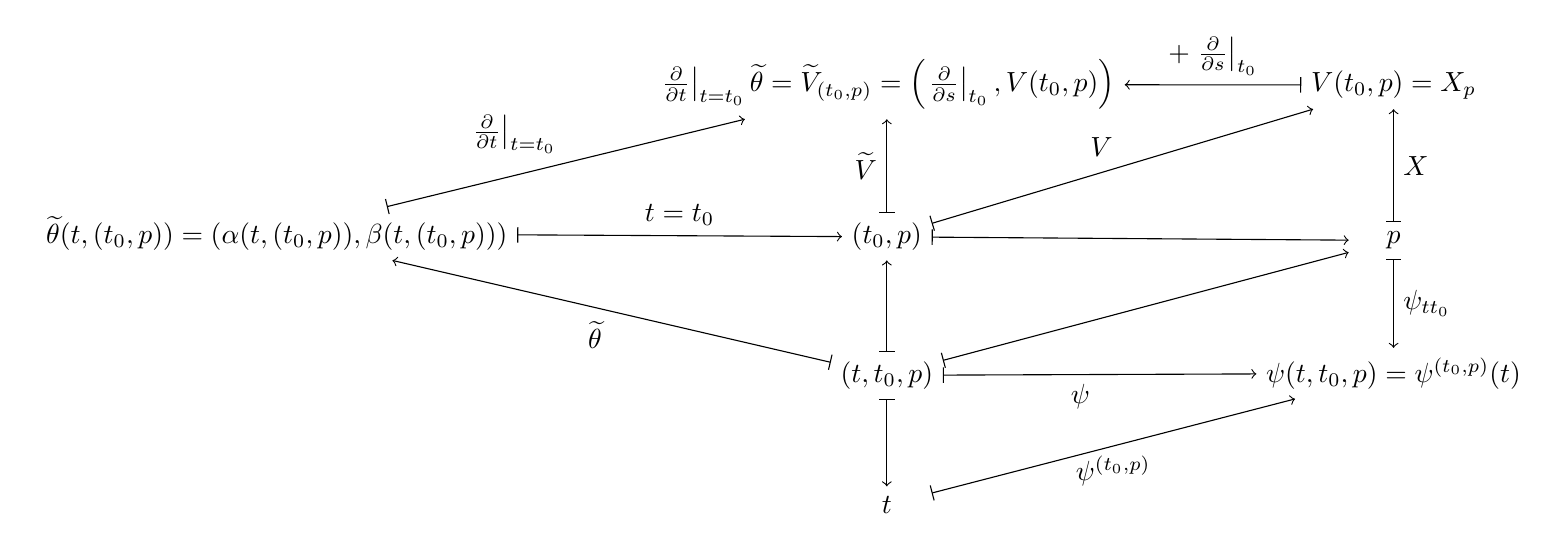
\begin{tikzpicture}
  \matrix (m) [matrix of math nodes, row sep=3.2em, column sep=4.8em, minimum width=3.2em]
  {
& \left. \frac{ \partial }{ \partial t} \right|_{t=t_0} \widetilde{\theta} = \widetilde{V}_{(t_0,p)} = \left( \left. \frac{ \partial }{ \partial s} \right|_{t_0}, V(t_0,p) \right) & V(t_0,p) = X_p  \\
\widetilde{\theta}(t,(t_0,p)) = (\alpha(t,(t_0,p)), \beta(t,(t_0,p)))  & (t_0,p)        & p  \\
& (t,t_0,p)       &       \psi(t,t_0,p) = \psi^{(t_0,p)}(t)  \\
& t & \\
};
  \path[|->]
 (m-2-2) edge node [left] {$\widetilde{V}$} (m-1-2)
         edge node [auto] {$V$} (m-1-3)
          edge node [above] {$$} (m-2-3)
  (m-3-2) edge node [auto] {$$} (m-2-2)
          edge node [auto] {$$} (m-2-3)
          edge node [below left] {$\psi$} (m-3-3)
          edge node [auto] {$$} (m-4-2)
          edge node [auto] {$\widetilde{\theta}$} (m-2-1)
  (m-4-2) edge node [below] {$\psi^{(t_0,p)}$} (m-3-3)
  (m-2-3) edge node [right] {$\psi_{tt_0}$} (m-3-3)
          edge node [right] {$X$} (m-1-3)
  (m-1-3) edge node [above] {$+ \left. \frac{\partial}{\partial s} \right|_{t_0}$} (m-1-2)
  (m-2-1) edge node [above] {$t=t_0$} (m-2-2)
          edge node [auto] {$\left. \frac{ \partial }{ \partial t} \right|_{t=t_0}$} (m-1-2)
; 
\end{tikzpicture}

with \[
\begin{gathered}
\left. \frac{ \partial }{ \partial t}\right|_{t=t_0} \widetilde{\theta}( t,(t_0,p)) = \left. \left( \frac{ \partial \alpha }{\partial t}(t,(t_0,p)), \frac{\partial \beta}{ \partial t}(t,(t_0,p))  \right)\right|_{t=t_0} = (1, V(t_0,p))
\end{gathered}
\]

EY : 20150725 I don't like Lee's choice of notation.  Let me rewrite the above diagrams:

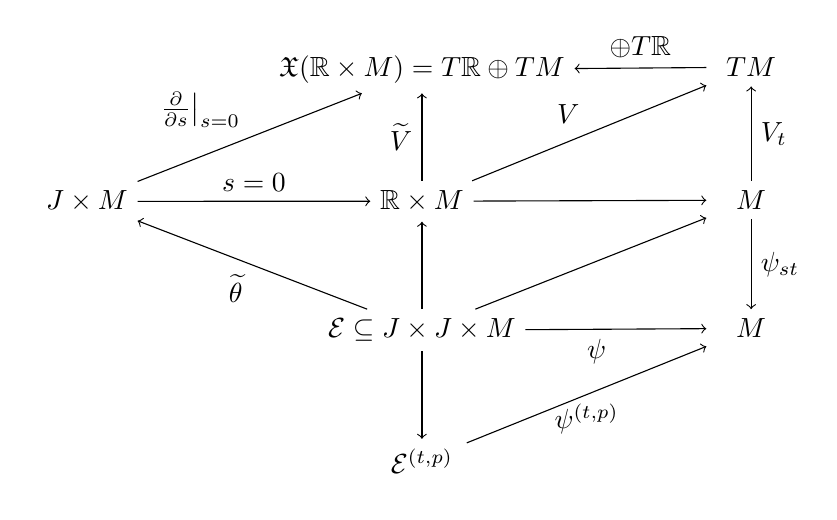
\begin{tikzpicture}
  \matrix (m) [matrix of math nodes, row sep=3.2em, column sep=4.8em, minimum width=3.2em]
  {
& \mathfrak{X}(\mathbb{R}\times M) = T\mathbb{R}\oplus TM     & TM   \\
J \times M & \mathbb{R} \times M &  M\\
& \mathcal{E} \subseteq J \times J \times M         &       M \\
& \mathcal{E}^{(t,p)}                            & \\
};
  \path[->]
  (m-2-2) edge node [left] {$\widetilde{V}$} (m-1-2)
         edge node [auto] {$V$} (m-1-3)
          edge node [above] {$$} (m-2-3)
  (m-3-2) edge node [auto] {$$} (m-2-2)
          edge node [auto] {$$} (m-2-3)
          edge node [below left] {$\psi$} (m-3-3)
          edge node [auto] {$$} (m-4-2)
          edge node [auto] {$\widetilde{\theta}$} (m-2-1)
  (m-4-2) edge node [below] {$\psi^{(t,p)}$} (m-3-3)
  (m-2-3) edge node [right] {$\psi_{st}$} (m-3-3)
          edge node [right] {$V_t$} (m-1-3)
  (m-1-3) edge node [above] {$\oplus T\mathbb{R}$} (m-1-2)
  (m-2-1) edge node [above] {$s=0$} (m-2-2)
          edge node [auto] {$\left. \frac{ \partial }{ \partial s} \right|_{s=0}$} (m-1-2)
;
\end{tikzpicture} \quad \quad \quad \, 

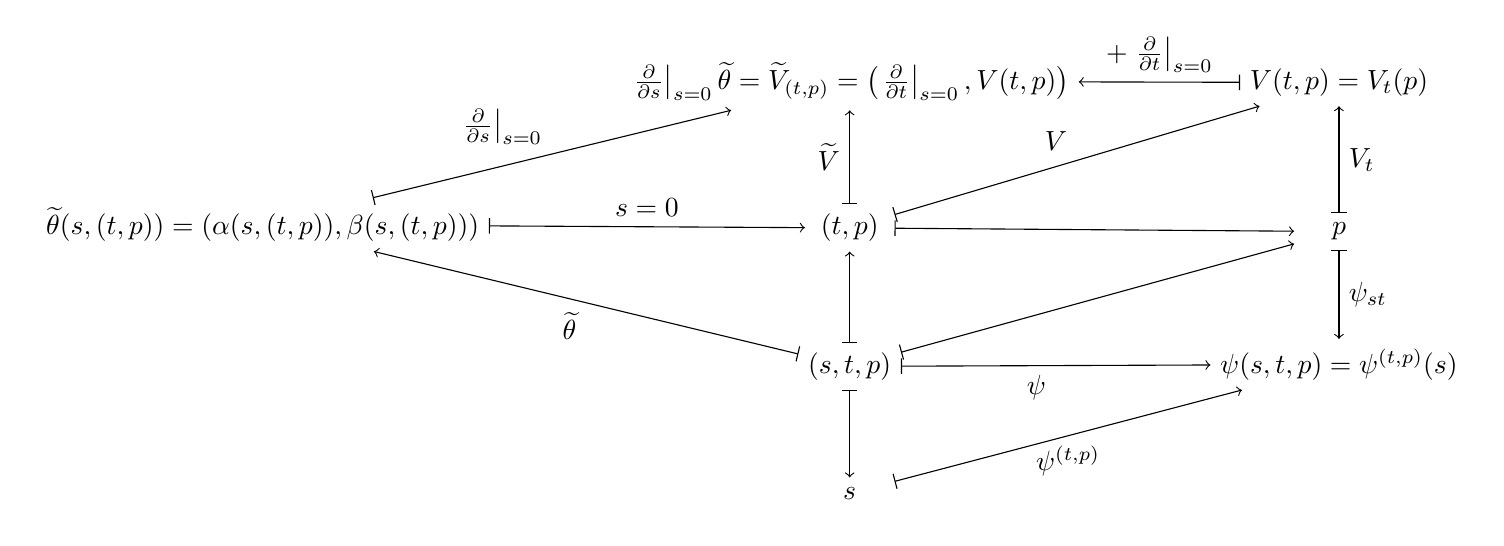
\begin{tikzpicture}
  \matrix (m) [matrix of math nodes, row sep=3.2em, column sep=4.8em, minimum width=3.2em]
  {
& \left. \frac{ \partial }{ \partial s} \right|_{s=0} \widetilde{\theta} = \widetilde{V}_{(t,p)} = \left( \left. \frac{ \partial }{ \partial t} \right|_{s=0}, V(t,p) \right) & V(t,p) = V_t(p)  \\
\widetilde{\theta}(s,(t,p)) = (\alpha(s,(t,p)), \beta(s,(t,p)))  & (t,p)        & p  \\
& (s,t,p)       &       \psi(s,t,p) = \psi^{(t,p)}(s)  \\
& s & \\
};
  \path[|->]
 (m-2-2) edge node [left] {$\widetilde{V}$} (m-1-2)
         edge node [auto] {$V$} (m-1-3)
          edge node [above] {$$} (m-2-3)
  (m-3-2) edge node [auto] {$$} (m-2-2)
          edge node [auto] {$$} (m-2-3)
          edge node [below left] {$\psi$} (m-3-3)
          edge node [auto] {$$} (m-4-2)
          edge node [auto] {$\widetilde{\theta}$} (m-2-1)
  (m-4-2) edge node [below] {$\psi^{(t,p)}$} (m-3-3)
  (m-2-3) edge node [right] {$\psi_{st}$} (m-3-3)
          edge node [right] {$V_t$} (m-1-3)
  (m-1-3) edge node [above] {$+ \left. \frac{\partial}{\partial t} \right|_{s=0}$} (m-1-2)
  (m-2-1) edge node [above] {$s=0$} (m-2-2)
          edge node [auto] {$\left. \frac{ \partial }{ \partial s} \right|_{s=0}$} (m-1-2)
; 
\end{tikzpicture}

with \[
\begin{gathered}
\left. \frac{ \partial }{ \partial s}\right|_{s=0} \widetilde{\theta}( s,(t,p)) = \left. \left( \frac{ \partial \alpha }{\partial s}(s,(t,p)), \frac{\partial \beta}{ \partial s}(s,(t,p))  \right)\right|_{s=0} = (1, V(t,p))
\end{gathered}
\]


\begin{theorem}[9.48] \textbf{(Fundamental Theorem on Time-Dependent Flows)} \\
Let $M$ smooth manifold \\
open $J \subseteq \mathbb{R}$ \\
$V: J \times M \to TM$ smooth time-dependent vector field on $M$ \\
$\exists \, $ open $\mathcal{E} \subseteq J\times J \times M$, smooth $\psi : \mathcal{E} \to M$ called time-dependent flow of $V$ s.t. 

\begin{enumerate}
\item[(a)] $\forall \, t_0 \in J$, \, $\forall \, p \in M$, \\
open $\mathcal{E}^{(t_0,p)} = \lbrace t \in J | (t,t_0, p) \in \mathcal{E}_0 \rbrace$ s.t. $t_0 \in \mathcal{E}^{(t_0, p)}$ \\
smooth curve $\begin{aligned}
  & \quad \\ 
  & \psi^{(t_0,p)}: \mathcal{E}^{(t_0,p)} \to M \\
  & \psi^{(t_0,p)}(t) = \psi(t,t_0,p) \end{aligned}$ \\
is unique maximal integral curve of $V$ with $\psi^{(t_0,p)}(t_0) = p$
\item[(b)] If $ \begin{aligned}
  & \quad \\ 
  & t_1 \in \mathcal{E}^{(t_0,p)} \\
  & q = \psi^{(t_0,p)}(t_1) \end{aligned}$

then $\begin{aligned}
  & \quad \\
  & \mathcal{E}^{(t_1,q)} = \mathcal{E}^{(t_0,p)} \text{ and } \\
  & \psi^{(t_1,q)} = \psi^{(t_0,p)} \end{aligned}$
\item[(c)] $\forall \, (t_1,t_0) \in J \times J $ \\
$M_{t_1,t_0} = \lbrace p \in M | (t_1,t_0, p) \in \mathcal{E} \rbrace$ open in $M$ and \\
  $\begin{aligned}
  & \quad \\
  & \psi_{t_1t_0} : M_{t_1t_0} \to M \\
  & \psi_{t_1t_0}(p) = \psi(t_1,t_0,p) \end{aligned}$
is a diffeomorphism from $M_{t_1t_0}$ onto $M_{t_0t_1}$ with inverse $\psi_{t_0t_1}$
\item[(d)] If $p \in M_{t_1t_0} $, $\psi_{t_1t_0}(p) \in M_{t_0t_1}$, \\
then $p\in M_{t_2 t_0}$ and 
\begin{equation}
\psi_{t_2t_1} \psi_{t_1t_0}(p) = \psi_{t_2t_0}(p) \quad \quad \quad \, (9.18)
\end{equation}
\end{enumerate}

\end{theorem}

\begin{proof}
Consider smooth vector field $\begin{aligned} 
& \quad  \\
  & \widetilde{V} \in \mathfrak{X}(J \times M ) \text{ defined by } \\
  & \widetilde{V}_{(s,p)} = \left( \left. \frac{ \partial }{ \partial s } \right|_s, V(s,p) \right) \end{aligned}$ \\

identify $T_{(s,p)}(J \times M)$ with $T_sJ \oplus T_pM$ (Prop. 3.14)

Let $\begin{aligned}
& \quad \\ 
  & \widetilde{\theta} : \widetilde{\mathcal{D}} \to J \times M \\
  & \widetilde{\theta}(t,(s,p)) = (\alpha(t,(s,p)) , \beta(t,(s,p)) ) \end{aligned}$ \quad \, flow of $\widetilde{V}$

then $\begin{aligned} 
 & \quad \\
  & \alpha: \widetilde{D} \to J \\
  & \beta: \widetilde{D} \to M \end{aligned}$ s.t. 

\[
\begin{aligned}
  & \frac{ \partial \alpha}{ \partial t}(t,(s,p) ) = 1 \quad \quad \, & \alpha(0,(s,p)) = s \\ 
  & \frac{ \partial \beta}{ \partial t}(t,(s,p)) = V(\alpha(t,(s,p)), \beta(t,(s,p))) \quad \quad \, & \beta(0,(s,p)) = p 
\end{aligned}
\]
$\Longrightarrow \alpha(t,(s,p)) = t+s$ so 
\begin{equation}
  \frac{ \partial \beta}{ \partial t}(t,(s,p)) = V(t+s,\beta(t,(s,p)) \quad \quad \quad \, (9.19)
\end{equation}
\end{proof}


Let $\begin{aligned}
  & \quad \\
  & \mathcal{E} \subseteq \mathbb{R} \times J \times M \text{ defined } \\
  & \mathcal{E} = \lbrace (t,t_0, p) | (t-t_0, (t_0,p) ) \in \widetilde{\mathcal{D}} \rbrace \end{aligned}$

$\mathcal{E}$ open because $\widetilde{\mathcal{D}}$ is. \\
since $\alpha: \widetilde{D} \to J$, if $(t,t_0, p) \in \mathcal{E}$, then $t= \alpha(t-t_0,(t_0,p)) \in J$, implies $\mathcal{E} \subseteq J \times J \times M$ \\
$\mathcal{E}$ open so $M_{t_1t_0} = \lbrace p \in M | (t_1,t_0, p) \in \mathcal{E} \rbrace$ open. 

define $\begin{aligned} & \quad \\ 
  & \psi : \mathcal{E} \to M \\
  & \psi(t,t_0,p) = \beta(t-t_0,(t_0,p))
\end{aligned}$

EY : 20150725 Remark: Out of the proof immediately above, there are a number of takeaways that really \emph{should} be mentioned.  

Let's collect the facts:
\[
\begin{aligned}
  & \widetilde{\theta}(s,(t,p)) = (\alpha(s,(t,p)), \beta(s,(t,p)) ) := \widetilde{\theta}^{(t,p)}(s) \\ 
  & \widetilde{\theta}(0,(t,p)) = (\alpha(0,(t,p)), \beta(0,(t,p)) ) = (t,p) \\ 
  & \frac{ \partial \alpha}{ \partial s}(s,(t,p)) = 1 \\
  & \frac{ \partial \beta }{ \partial s}(s,(t,p)) = V(\alpha(s,(t,p)), \beta(s,(t,p))) \text{ so } \\ 
  & \alpha(s,(t,p)) = s+t \\ 
  & \frac{ \partial \beta}{ \partial s}(s,(t,p)) = V(s+t,\beta(s,(t,p)) ) \\
  & \left. \frac{ \partial }{ \partial s} \right|_{s=0} \widetilde{\theta}(s,(t,p)) = \left. \left( \frac{ \partial \alpha }{ \partial s}(s,(t,p)) , \frac{ \partial \beta}{ \partial s}(s,(t,p)) \right) \right|_{s=0} = (1,V(t,p)) = \frac{d\widetilde{\theta}^{(t,p)}}{ds}(s=0) := \widetilde{V}_{(t,p)}
\end{aligned}
\]

Also, we can write the flow $\widetilde{\theta}_s$ as
\[
\widetilde{\theta}^{(t,p)}(s) = \widetilde{\theta}(s,(t,p)) = \widetilde{\theta}_s(t,p) = (\alpha(s,(t,p)),\beta(s,(t,p))) = (s+t, \beta(s,(t,p)))
\]

Now consider the Lie derivative:

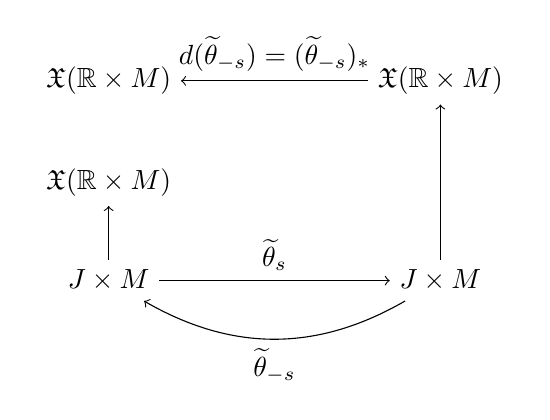
\begin{tikzpicture}
  \matrix (m) [matrix of math nodes, row sep=2em, column sep=6.8em, minimum width=2em]
  {
\mathfrak{X}(\mathbb{R} \times M) & \mathfrak{X}(\mathbb{R} \times M)  \\
\mathfrak{X}(\mathbb{R} \times M) &   \\
J\times M    &       J\times M \\
};
  \path[->]
  (m-3-1) edge node [above] {$$} (m-2-1)
  edge node [above] {$\widetilde{\theta}_s$} (m-3-2)
  (m-3-2) edge node [auto] {$$} (m-1-2)
  edge [bend left] node [auto] {$\widetilde{\theta}_{-s}$} (m-3-1)
  (m-1-2) edge node [above] {$d(\widetilde{\theta}_{-s})=(\widetilde{\theta}_{-s})_*$} (m-1-1)
;
\end{tikzpicture} \quad \quad \quad \, 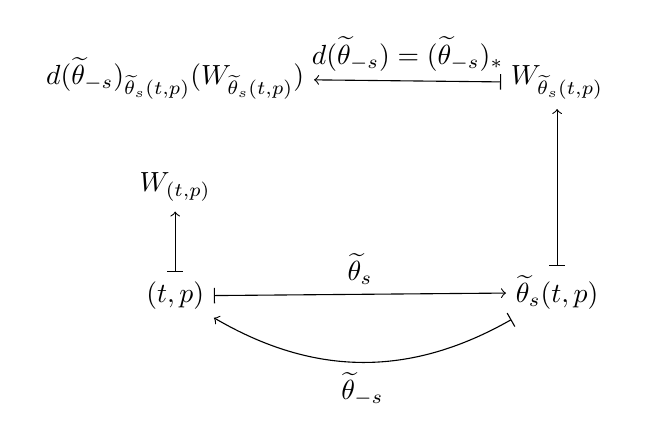
\begin{tikzpicture}
  \matrix (m) [matrix of math nodes, row sep=2em, column sep=6.8em, minimum width=2em]
  {
d(\widetilde{\theta}_{-s})_{\widetilde{\theta}_s(t,p)}(W_{\widetilde{\theta}_s(t,p)}) & W_{\widetilde{\theta}_s(t,p)}  \\
W_{(t,p)}   &    \\
(t,p)    &       \widetilde{\theta}_s(t,p) \\
};
  \path[|->]
  (m-3-1) edge node [above] {$$} (m-2-1)
  edge node [above] {$\widetilde{\theta}_s$} (m-3-2)
  (m-3-2) edge node [auto] {$$} (m-1-2)
  edge [bend left] node [auto] {$\widetilde{\theta}_{-s}$} (m-3-1)
  (m-1-2) edge node [above] {$d(\widetilde{\theta}_{-s})=(\widetilde{\theta}_{-s})_*$} (m-1-1)
;
\end{tikzpicture}

with $\widetilde{\theta}$ being the flow of $\widetilde{V}$.  Let's define the Lie derivative:

\begin{equation}
\begin{gathered}
  \mathcal{L}_{\widetilde{V}}W = (\mathcal{L}_{\widetilde{V}}W)_{(t,p)} = \left. \frac{d}{ds} \right|_{s=0}(d\widetilde{\theta}_{-s})_{\widetilde{\theta}_s(t,p)}(W_{\widetilde{\theta}_s(t,p)})   = \lim_{s\to 0} \frac{ (d\widetilde{\theta}_{-s})_{\widetilde{\theta}_s(t,p)}( W_{\widetilde{\theta}_s(t,p)}) - W_{\widetilde{\theta}_s(t,p)} }{s}
\end{gathered}
\end{equation}


Use Case 1 of the proof of Lee's Theorem 9.38, for showing $\mathcal{L}_VW = [V,W]$.  \\
Let open neighborhood $U \subseteq J \times M$, with $(t,p) \in U$.  On open $U$, choose smooth coordinates $(t,u^i)$ on $U$.  By Theorem 9.22, that at a regular point $p\in M$, $\exists \, (u^i)$ coordinates s.t. $V_p = \frac{ \partial }{ \partial u^1}$, then consider 

\[
\widetilde{V} = \frac{ \partial }{ \partial t} + \frac{ \partial }{ \partial u^1} \in \mathfrak{X}(\mathbb{R} \times M)
\]
with $V(t)(p) = \frac{ \partial }{ \partial u^1} \in \mathfrak{X}(M)$.  (Remember, $V(t)$ is a vector-field that is time-dependent, but is on $M$.  I will use this as a justification for using Thm. 9.22).  

Now the flow $\widetilde{\theta}_s$ takes on these forms:
\[
\begin{gathered}
  \widetilde{\theta}^{(t,p)}(s) = \widetilde{\theta}(s,(t,p)) = \widetilde{\theta}_s(t,p) = \\
  = (\alpha(s,(t,p)) , \beta(s,(t,p))) = (s+t, \beta(s,(t,p)) )
\end{gathered}
\]
Given these conditions, that \\
$\beta(0,(t,p)) = p = (u^1,u^2, \dots u^n)$ and 
\[
\left. \frac{ \partial \beta}{ \partial s}(s, (t,p)) \right|_{s=0} = V(t,p) = \frac{ \partial }{ \partial u^1} = \left. \frac{d}{ds} \beta^{(t,p)}(s) \right|_{s=0}
\]
then a $\beta$ that satisfies these conditions above is 
\[
\beta(s,(t,p)) = \beta_s(t,p) = (u^1 + s, u^2 \dots u^n)
\]
so that we can conclude that 
\[
\widetilde{\theta}_s(t,p) = (t+s, u^1 + s, u^2 , \dots , u^n)
\]

For fixed $s$, then
\[
d(\widetilde{\theta}_{-s})_{\widetilde{\theta}_s(t,p)} =1_{T_{\widetilde{\theta}_s(t,p)}(\mathbb{R}\times M)}
\]
so that 
\[
\begin{gathered}
  d(\widetilde{\theta}_{-s})_{\widetilde{\theta}_s(t,p)}(W_{\widetilde{\theta}_s(t,p)}) = d(\widetilde{\theta}_{-s})_{\widetilde{\theta}_s(t,p)} \cdot W^j(t+s,u^1 +s, u^2 \dots u^n) \left. \frac{ \partial }{ \partial u^j} \right|_{\widetilde{\theta}_s(t,p)} = W^j(t+s,u^1+s, u^2 \dots u^n) \left. \frac{ \partial }{ \partial u^j} \right|_{(t,p)} \\
\Longrightarrow \left. \frac{d}{ds} \right|_{s=0} W^j(t+s,u^1+s, u^2 \dots u^n) \left. \frac{ \partial }{ \partial u^j} \right|_{(t,p)} = \left( \frac{\partial }{ \partial t} W^j(t,u^1 \dots u^n) + \frac{ \partial }{ \partial u^1 } W^j(t,u^1 \dots u^n) \right) \left. \frac{ \partial}{ \partial u^j} \right|_{(t,p)}
\end{gathered}
\]


Thus, we can conclude that 
\begin{equation}
  \boxed{ \mathcal{L}_{\widetilde{V}}W = \mathcal{L}_{ \frac{ \partial }{ \partial t} +V}W = \left( \mathcal{L}_{ \frac{ \partial}{ \partial t} V } W \right)_{(t,p)} = \left( \left( \frac{ \partial }{ \partial t} + V \right) W^j \right) \left. \frac{ \partial }{ \partial x^j} \right|_{(t,p)} }
\end{equation}

\subsection*{First-Order Partial Differential Equations }



\subsection*{ Problems }


\problemhead{9-21} Note that from wikipedia, 

ambient isotopy \\
Let $N, M$ manifolds, \\
\quad $g,h$ embeddings of $N$ in $M$ 

cont. map $F: M \times [0,1] \to M$ s.t.  \\
$F: g\mapsto h$ \\
if $F_0 = 1$ \\
\phantom{ if } $F_t$ homeomorphism, $F_t: M \to M$ \\
\phantom{ if } $F_1 : g \mapsto h$ \\

\textbf{smooth isotopy} of $M$ is smooth $H: M \times J \to M$, \, $J \subseteq R$ interval s.t. \\
\quad \, $\forall \, t \in J$, $\begin{aligned} & \quad \\
  & H_t : M \to M \\
  & H_t(p) = H(p,t) \end{aligned}$ is a diffeomorphism.  

Suppose open interval $J \subseteq \mathbb{R}$ \\
\phantom{Suppose } smooth isotopy $H:M \times J \to M$ \\

EY : 20140206 

By definition \\
$\forall \, t, \, \begin{aligned} & \quad \\
  & H_t : M \to M \\
  & H_t(p) = H(p,t) \end{aligned}$

Then $DH_t = (H_t)_*$ \\
\[
DH_t : TM \to TM
\]

I tried, 

for some time $t$, consider $H(x^i(p),t) = y^j(x^i,t)$ 
\[
\frac{ \partial H(p,t)}{ \partial t } = \frac{ \partial y^j(x^i,t) }{ \partial t }
\]

Consider integral curve $x = x(t)$ s.t. $\dot{x} = X(t)$ 

\[
\begin{gathered}
  \dot{y} = \frac{dy}{dt} = \frac{d}{dt} y(x(t),t) = \frac{ \partial y^j}{ \partial x^i }\dot{x}^i = (DH_t)X \\
\begin{aligned}
  & (H_t)_* : TM \to TM \\ 
  & DH_t : X \mapsto \dot{y} = Y
\end{aligned}
\end{gathered}
\]



$\psi(t,t_0,p) = H_t \circ H_{t_0}^{-1}(p)$ domain $J \times J \times M$ ??





\section{Vector Bundles }

\subsection*{Vector Bundles }

\textbf{ (real) vector bundle of rank $k$ over $M$ } is topological space $E$, \\
\quad surjective cont. $\pi: E \to M$ s.t.
\begin{enumerate}
\item[(i)] $\forall \, p \in M$, $E_p = \pi^{-1}(p)$ endowed with structure of $k$-dim. real vector space
\item[(ii)] $\forall \, p \in M$, \\
  $\exists \, $ neighborhood $U \ni p$ \\
  $ \exists \, $ homeomorphism $\Phi : \pi^{-1}{(U)} \to U \times \mathbb{R}^k$ (local trivialization of $E$ over $U$) \\

s.t. 

\begin{itemize}
\item $\pi_U \circ \Phi = \pi$ (where $\pi_U : U \times \mathbb{R}^k \to U$) 
\item $\forall \, q\in U$, $\left. \Phi \right|_{E_q}$ is vector space isomorphism from $E_q$ to $\lbrace q \rbrace \times \mathbb{R}^k \cong \mathbb{R}^k$
\end{itemize}
\end{enumerate}

if $M, E$ smooth manifolds with or without boundary, $\pi$ smooth, local trivializations $\Phi$ can be chosen to be diffeomorphisms, \\
$E$ \textbf{smooth vector bundle}, \\
$\forall \, \Phi$ that's a diffeomorphism onto its image a \textbf{ smooth local trivialization} \\

(real) line bundle - rank 1 vector bundle 

complex vector bundle - $\mathbb{R}^k$ replaced by $\mathbb{C}^k$

\exercisehead{10.1} Suppose $E$ smooth vector bundle over $M$. \\
$\pi$ surjective by def.  

EY : 20140204

submersion at $p \in M$, $F$, if for differentiable manifolds $M, N$, differentiable $F: M \to N$, \\
\quad differential $DF_p : T_p M \to T_{F(p)}N$ \\
\quad \, is surjective \\

By def., $\forall \, p \in M$, $\exists \, U, \Phi$ \\
\quad $\Phi$ vector space isomorphism and can be chosen to be diffeomorphism \\
\quad $\Phi$ diffeomorphism if $\Phi$ bijection, $\Phi^{-1}$ differentiable \\

$\begin{aligned}
& \quad \\ 
  & \Phi: \pi^{-1}(U) \to U \times \mathbb{R}^k \\
  & D\Phi : T\pi^{-1}(U) \to T(U \times \mathbb{R}^k ) = TU \times T\mathbb{R}^k 
\end{aligned}$ \\

$\begin{aligned} 
  & \quad \\
  & \pi_U : U \times \mathbb{R}^k \to U \\
  & D\pi_U : T(U \times \mathbb{R}^k ) \to TU \end{aligned}$  \\

$\begin{gathered}
\pi:\pi^{-1}(U) \to U \\
\pi = \pi_U \circ \Phi \end{gathered}$ \\

So by chain rule, 

\[
D\pi = D\pi_U D\Phi
\]
\[
D\pi : T\pi^{-1}(U) \to TU
\]
$D\pi_U$ clearly a surjection.  

$D\Phi$ bijection. 

So $D\pi$ a surjection.  

\hrulefill

\section{The Cotangent Bundle}

\subsection*{Covectors}

\exercisehead{11.2} For linear $\omega : V \to \mathbb{R}$, $\omega \in V^*$ 
\[
\begin{gathered}
\omega(E_j) = \omega( \delta^i_{ \, j} E_i) = \delta^i_{ \, j } \omega(E_i) = \omega(E_i) \epsilon^i(E_j) \\
\Longrightarrow \omega = \omega(E_i)\epsilon^i
\end{gathered}
\]
So $\omega$ spanned by $\epsilon^i$, \, $i = 1 \dots n$

Suppose $0 = \omega_i \epsilon^i$.  Then $\forall \, x \in V$, \[
\omega_i \epsilon^i(x^j E_j) = \omega_i x^j \delta^i_{ \, j } = \omega_i x^i = \omega(E_i) x^i = \omega(x) = 0 
\]
Then $\omega=0$ since $\omega(x) =0, \, \forall\, x \in V$.  So $\epsilon^i$ form a linear basis of $V^*$.  

By theorem, $\text{dim}{ V^*} = \text{dim}{V}$



\section{Lie Group Actions}

\subsection{ Group Actions }

action $G$ on $M$ cont. if $\begin{aligned} & \quad \\ & G \times M \to M \\ & (g,p) \mapsto gp \end{aligned}$ or $\begin{aligned} & \quad \\ & M \times G \to M \\ & (p,g) \mapsto pg \end{aligned}$ cont.  

For cont. action, $\theta_g$ homeomorphism, since $\exists \, $ cont. inverse $\theta_{g^{-1}}$.  $\theta_g : M \to M$

orbit \\
$\forall \, p \in M$, orbit of $p = Gp = \lbrace gp | g \in G \rbrace$ 

action $\theta$ transitive if $\forall \, p, q \in M$, $\exists \, g$ s.t. $gp = q$, i.e. $Gp = M$

isotropy group of $p$, $G_p = \lbrace g \in G | gp = p \rbrace$ 

action $\theta$ is free if the only element of $G$ that fixes any element of $M$ is $e$, \\
i.e. if $g \cdot p = p$, $ p \in M$, $g=e$.  \\ 
i.e. $G_p = 1$ \, $\forall \, p \in M$

Example 9.1 (Lie Group Actions)
\begin{enumerate}
\item[(a)] trivial action of $G$ on $M$ is $gp = p$ \, $\forall \, g \in G$, \, $G_p = G$
\item[(b)] action of $GL(n,\mathbb{R}) $ on $\mathbb{R}^n$, $(A,x) \mapsto Ax$; $x \in \mathbb{R}^n$ column matrix.  \\
$Ax $ smooth, because components of $Ax$ depend polynomially on matrix entries of $A$ and components of $x$.  \\
Exactly only 2 orbits : $0, \mathbb{R}^n - 0$ \, ($\forall \, y =0$, $y\in \mathbb{R}^n$, $\begin{aligned} & \quad \\ 
  & Ax  =y \\ 
  & x = A^{-1}y \end{aligned}$ ) 
\item[(c)] $O(n) \times \mathbb{R}^n \to \mathbb{R}^n$  \\
orbits : $0, S^{n-1}(R)$, \, $\forall \, R >0$.  To show this, complete $\frac{v}{ |v|}, \frac{v'}{|v'|}$, \, $\forall \, v , v' \neq 0$, to orthonormal bases.  Let $A, A'$ columsn be these orthonormal bases 
\[
A' A^{-1}(v) = v'
\]
\item[(d)] $O(n) \times S^{n-1} \to S^{n-1}$.  $O(n)$ transitive action of $O(n)$ on $S^{n-1}$.  \\
action $O(n) \times S^{n-1} \to S^{n-1}$ smooth by Corollary 8.25, $S^{n-1}$ embedded submanifold of $\mathbb{R}^n$

\end{enumerate}





\subsubsection*{Representations}

If $G$ Lie group, \\
(finite-dim.) representation of $G$ is a Lie group homomorphism 
\[
\rho : G \to GL(V)
\]
$\forall \, $ representation $\rho$ yields or smooth left action of $G$ on $V$, 
\[
g\cdot v = \rho(g) v , \quad \quad \, \forall \, g \in G, \, v \in V
\]


\subsection*{Equivariant Maps }

\subsection*{Proper Actions}

\subsection*{Quotient of Manifolds by Group Actions}

Suppose Lie group $G$ acts on manifold $M$ \\
$p\sim q$ if $\exists \, g \in G$ s.t. $gp = q$ \quad equivalence classes are exactly the orbits of $G$ in $M$  

$M/G$ set of orbits, with quotient topology, orbit space of the action





\section{Tensors}
% 12tensors.tex
% Fund Science! & Help Ernest finish his Physics Research! : quantum super-A-polynomials - a thesis by Ernest Yeung
%                                               
% http://igg.me/at/ernestyalumni2014                                                                             
%                                                              
% Facebook     : ernestyalumni  
% github       : ernestyalumni                                                                     
% gmail        : ernestyalumni                                                                     
% google       : ernestyalumni                                                                                   
% linkedin     : ernestyalumni                                                                             
% tumblr       : ernestyalumni                                                               
% twitter      : ernestyalumni                                                             
% youtube      : ernestyalumni                                                                
% indiegogo    : ernestyalumni                                                                        
%
% Ernest Yeung was supported by Mr. and Mrs. C.W. Yeung, Prof. Robert A. Rosenstone, Michael Drown, Arvid Kingl, Mr. and Mrs. Valerie Cheng, and the Foundation for Polish Sciences, Warsaw University.                  



\subsection*{ Multilinear Algebra }



$F: V_1 \times \dots \times V_k \to W$ multilinear if $\forall \, i$, linear in each variable, $F(v_1 \dots a v_1 + a' v_i' \dots v_k) = aF(v_1 \dots v_i \dots v_k) + a'F(v_1 \dots v_i' \dots v_k)$

multilinear function of 2 variables is bilinear.  \\

$L(V_1, \dots V_k; W)$ - set of all multilinear maps from $V_1 \times \dots \times V_k$ to $W$ \\

$\lbrace T: \underbrace{V\times \dots \times V}_{k \text{times }} \to \mathbb{R} \rbrace = T^k(V)$  \\

$S\in T^k(V), \, T\in T^l(V)$  \\
tensor product $S\otimes T: V \times \dots \times V \to \mathbb{R}$, covariant $(k+l)$-tensor

\[
  S \otimes T(x_1 \dots x_{k+l}) = S(x_1 \dots x_k) T(x_{k+1} \dots x_{k+l}) \\ 
\]

\exercisehead{12.3}  
\[
\begin{gathered}
  F(v_1 \dots av_i + bw_i \dots v_k) G(v_{k+1} \dots v_{k+l}) = aF(v_1 \dots v_i \dots v_k) G + b F(v_1 \dots w_i \dots v_k)G = \\
  =  aF\otimes G(v_1 \dots v_i \dots v_k \dots v_{k+l}) + bF\otimes G(v_1 \dots w_i \dots v_k \dots v_{k+l}) = F\otimes G( v_1 \dots a v_i  + b w_i \dots v_k, v_{k+1} \dots v_{k+l} ) \\ 
    F(v_1 \dots v_k) G(v_{k+1} \dots av_{k+i} + bw_{k+i} \dots v_{k+l}) = \\
    = F(v_1 \dots v_k)(aG(v_{k+1} \dots v_{k+i}, v_{k+i +1} \dots v_{k+l} ) + bG(v_{k+1 } \dots w_{k+i} v_{k+i +1} \dots v_{k+l }) = \\ 
    = aF\otimes G(v_{k+1} \dots v_{k+i} , v_{k+i +1} \dots v_{k+l }) + bF\otimes G(v_1 \dots w_{k+i}, v_{k+i + 1} \dots v_{k+l} ) = \\
    = F\otimes G(v_1 \dots v_k, v_{k+1} \dots av_{k+i} + b w_{k+i} \dots v_{k+i +1} \dots v_{k+l })
\end{gathered}
\]

\[
\begin{gathered}
(F\otimes G) \otimes H = (F\otimes G)(x_1 \dots x_{k+l}H(x_{k+l+1} \dots x_{k+l+m }) = F(x_1 \dots x_k) G(x_{k+1} \dots x_{k+l} ) H(x_{k+l+1} \dots x_{k+l+m}) = \\
= F(x_1 \dots x_k)(G\otimes H)(x_{k+1} \dots x_{k+l+m}) = F\otimes (G\otimes H)(x_1 \dots x_{k+l+m})
\end{gathered}
\]


\begin{proposition}[12.4](A Basis for the Space of Multilinear Functions)  Let $V$ real vector space of dim. $n$, $(E_i)$ any basis for $V$, $\epsilon^i$ dual basis.\\
set of all $k$-tensors of form $\epsilon^{i_1} \otimes \dots \otimes \epsilon^{i_k}$, \, $1\leq i_1 \dots i_k \leq n$ basis for $T^k(V)$, \, dim. $n^k$
\end{proposition}

\begin{proof} Let $\mathcal{B} = \lbrace \epsilon^{i_1} \otimes \dots \otimes \epsilon^{i_k} | 1 \leq i_1 \dots i_k \leq n \rbrace$ \\

Suppose arbitrary $T \in T^k(V)$  \\
Define $T_{i_1 \dots i_k} = T(E_{i_1} \dots E_{i_k} )$

\[
T_{i_1 \dots i_k} \epsilon^{i_1} \otimes \dots \otimes \epsilon^{i_k}(E_{j_1} \dots E_{j_k} ) \underbrace{=}_{ \text{ (by definition) } }T_{i_1 \dots i_k} \epsilon^{i_1}(E_{j_1}) \dots \epsilon^{i_k}(E_{j_k}) = T_{i_1 \dots i_k}\delta^{i_1}_{j_1} \dots \delta^{i_k}_{j_k} = T_{j_1 \dots j_k} = T(E_{j_1} \dots E_{j_k} )
\]
$T$ spanned by $\mathcal{B}$

\end{proof}





\subsubsection*{ Abstract Tensor Products of Vector Spaces }



free vector space on $S$, $\mathbb{R}\langle S \rangle = \lbrace \mathcal{F} \rbrace$ \\
\quad \quad finite formal linear combination - function $\mathcal{F} : S \to \mathbb{R}$ s.t. $\mathcal{F}(s) = 0$ for all but finite many $s \in S$ \\
\quad \quad $\forall \, \mathcal{F} \in \mathbb{R} \langle S \rangle$, $\mathcal{F} = \sum_{i=1}^m a_i x_i$, \, $x_1 \dots x_m \in S$ s.t. $\mathcal{F}(x_i) \neq 0$, $a_i = \mathcal{F}(x_i)$

\exercisehead{12.6} (Characteristic Property of Free Vector Spaces)

\[
\begin{aligned}
  F : S & \to W \\ 
  & x \mapsto w \in W 
\end{aligned}
\]
Consider $w\in W$ and $w = \sum c_{\alpha} w_{\alpha}$, $w_{\alpha} = F(x_{\alpha})$; $x_{\alpha} \in S$, $w_{\alpha} \in W$.  

Consider $\overline{F}:\mathbb{R}\langle S \rangle \to W$, \, $\sum_{i=1}^m c_i x_i \mapsto \sum_{I=1}^m c_i F(x_i) = \sum_{i=1}^m c_i w_i \in W$

Let $w= v$, $\begin{aligned} & \quad \\ & w = \sum_{I=1}^m c_i w_i = \sum_{i=1}^m c_i F(x_i) \\ & v = \sum_{i=1}^n b_i v_i = \sum_{i=1}^n b_i F(y_i) \end{aligned}$

$w - v =0$ so for a vector space, this implies $w_i = v_i$, $m=n$, 
\[
\sum_{i=1}^m (c_i-b_i)w_i = 0, \quad \quad c_i = b_i
\]

$\mathcal{R} \equiv$ subspace of free vector space $\mathbb{R}\langle V \times W \rangle $ spanned by 
\begin{equation}
\begin{gathered}
  a(v,w) - a(v, w) \\
  a(v,w) - (v,aw) \\
(v,w) + (v',w) - (v+v',w) \\
  (v,w) + (v,w') - (v,w+w')
\end{gathered} (12.4)
\end{equation}

tensor product of $V, W$ 
\[
V\otimes W = \mathbb{R} \langle V \times W \rangle / \mathcal{R}
\]
equivalence class of element $(v,w)$ if $v\otimes w \in V\otimes W$

\begin{proposition}[12.7] (Characteristic Property of the Tensor Product Space)
  If bilinear $A: V \times W \to X$, $\exists \, !, \, \widetilde{A} : V\otimes W \to X$, any vector space $X$  s.t.
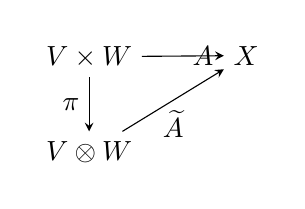
\begin{tikzpicture}
  \matrix (m) [matrix of math nodes, row sep=2em, column sep=3em, minimum width=1em]
  {
    V\times W  & X  \\
    V\otimes W  &   \\ };
  \path[-stealth]
  (m-1-1) edge node [right] {$A$} (m-1-2)
  edge node [left] { $\pi$} (m-2-1)
  (m-2-1) edge node [below] {$\widetilde{A}$} (m-1-2);
\end{tikzpicture}  (12.6)

$\pi(v,w) = V\otimes W$
\end{proposition}

\begin{proof}
By characteristic property of free vector space, $A: V\times W \to X$ extends uniquely to linear $\overline{A} : \mathbb{R} \langle V \times W \rangle \to X$

\[
\overline{A}(v,w) = A(v,w) \text{ if } (v,w) \in V\times W \subset \mathbb{R}\langle V \times W \rangle
\]

$A$ bilinear

\[
\begin{aligned}
  \overline{A}(av,w) = A(av,w) = aA(v,w) = a\overline{A}(v,w) = \overline{A}(a(v,w)) \\ 
  \overline{A}(v,aw) = A(v,aw) = aA(v,w)  = \overline{A}(a(v,w)) \\ 
  \overline{A}(v+v',w)  = A(v+v',w) = A(v,w) +  A(v',w) = \overline{A}(v,w) = \overline{A}(a(v',w)) \\ 
\end{aligned}
\]
\end{proof}

Likewise for (12.4) 

subspace $\mathcal{R} \subset \text{ker}{\overline{A}}$

$\therefore \, \overline{A}$ descends to linear $\widetilde{A} : V\otimes W = \mathbb{R} \langle V\times W \rangle / \mathcal{R} \to X$ s.t. \\
$\widetilde{A} \circ \pi = \overline{A}$, $\pi: \mathbb{R}\langle V \times W \rangle \to V\otimes W$

uniqueness from $\forall \, v \otimes w \in V \otimes W$, $v\otimes w =$ linear combination of $v\otimes w$ \\
$\widetilde{A}$ uniquely determined on $\widetilde{A}(v\otimes w) = \overline{A}(v,w) = A(v,w)$


\begin{proposition}[11.4] (\textbf{Other Properties of Tensor Products}).  Let $V, W$, and $X$ be finite-dimensional real vector spaces 
\begin{enumerate}
  \item[(a)] $V^* \otimes W^*$ canonically isomorphic to $B(V,W)$, bilinear maps from $V\times W$ into $\mathbb{R}$
  \item[(b)] if $\begin{aligned} & \quad \\ & (E_i) \text{ basis for $V$ } \\ & (F_j) \text{ basis for $W$ } \end{aligned}$, then $\lbrace E_i \otimes F_j \rbrace$ basis is basis for $V\otimes W$, $\therefore \, \text{dim}{(V\otimes W)} = \text{dim}{V} \text{dim}{W}$
  \item[(c)] $\exists \, !$ \, isomorphism $\begin{aligned} & \quad \\ & V\otimes (W\otimes X) \to (V \otimes W) \otimes X \\ & v\otimes (w \otimes x) \mapsto (v\otimes w)\otimes x \end{aligned}$
\end{enumerate}
\end{proposition}



\begin{proof}
\begin{enumerate}
\item[(a)] canonical isomorphism (basis independence) construction between $V^* \otimes W^*$ and $B(V,W)$ (space of bilinear maps) \\

Define $\begin{aligned} & \quad \\
  & \Phi : V^* \times W^* \to B(V,W) \\
  & \Phi(\omega, \eta)(v,w) = \omega(v) \eta(\omega) \end{aligned}$

$\Phi$ bilinear (easy to check).  

Prop. 11.3  $\forall \, $ bilinear $A: V\times W \to X$, $\exists \, ! \widetilde{A} : V\otimes W \to X$, any vector space $X$ s.t. $\widetilde{A} \pi = A$

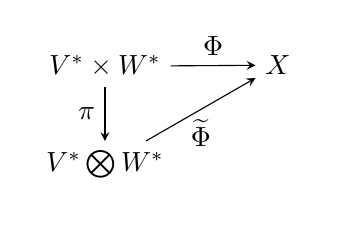
\begin{tikzpicture}
  \matrix (m) [matrix of math nodes, row sep=2em, column sep=3em, minimum width=1em]
  {
    V^*\times W^*  & X  \\
    V^* \bigotimes W^*  &   \\ };
  \path[-stealth]
  (m-1-1) edge node [auto] {$\Phi$} (m-1-2)
  edge node [left] { $\pi$} (m-2-1)
  (m-2-1) edge node [below] {$\widetilde{\Phi}$} (m-1-2);
\end{tikzpicture} 

i.e. descends uniquely to linear $\widetilde{\Phi} : V^* \otimes W^* \to B(V,W)$

Let $\begin{aligned} & \quad \\
  & (e_i) \\ 
  & (f_j) \end{aligned}$ be bases for $\begin{aligned} & \quad \\ 
  & V, \\
  & W \end{aligned}$ \quad $\begin{aligned} & \quad \\ 
  & (\epsilon^i) \\ 
  & (\phi^j) \end{aligned}$ \quad dual basis 

since $V^* \otimes W^*$ spanned by elements of the form $\omega \otimes \eta$, $\begin{aligned} & \quad \\ & \omega \in V^* \\
 & \eta \in W^* \end{aligned}$ \\
$\forall \, \tau \in V^* \otimes W^*$, \, $\tau = \tau_{ij} \epsilon^i \otimes \varphi^j $

Define $\begin{aligned} & \quad \\
  & \Psi : B(V, W) \to V^* \otimes W^* \\
  & \Phi(b) = b(e_k,  f_l) \epsilon^k \otimes \varphi^l 
\end{aligned}$

\[
\begin{gathered}
  \Psi \widetilde{\Phi}(\tau) = \widetilde{\Phi}(\tau)(e_k , f_l) \epsilon^k \otimes \varphi^l = \tau_{ij} \widetilde{\Phi}(\epsilon^i \otimes \varphi^j)(e_k , f_l) \epsilon^k \otimes \varphi^l = \tau_{ij} \Phi( \epsilon^i , \varphi^j) (e_k , f_l) \epsilon^k \otimes \varphi^l = \\
= \tau_{ij} \epsilon^i(e_k) \varphi^j(f_l) \epsilon^k\otimes \varphi^l = \tau_{kl} \epsilon^k \otimes \varphi^l = \tau
\end{gathered}
\]

For $\begin{aligned} & \quad \\ 
  & v \in V \\ 
  & w \in W \end{aligned}$
\[
\begin{gathered}
  \widetilde{\Phi} \circ \Psi(b)(v,w) = \widetilde{\Phi} b(e_j,f_k) \epsilon^j \otimes \varphi^k(v,w) = b(e_j , f_k) \widetilde{\Phi}(\epsilon^j \otimes \varphi^k)(v,w) = \\
  = b(e_j, f_k) \Phi(e^i, \varphi^k)(v,w) = b(e_j, f_k) e^i(v) \varphi^k(w) = b(e_j, f_k) v^i \varphi^k = b(v,w)
\end{gathered}
\]

\item[(b)]
Given $\begin{aligned}
  & \lbrace e_i | i \in I \rbrace = \mathcal{B}_U \\ 
  & \lbrace f_j | j \in J \rbrace = \mathcal{B}_U \\ 
\end{aligned}$

By the bilinearity of tensor product: $a_i e_i \otimes b_j f_j  = a_i b_j e_i \otimes f_j$ 

Consider dual basis elements $\begin{aligned} & \quad \\
  & e^*_k(e_i) = \delta_{ik} \\
   & f^*_l(f_j) = \delta_{jl} \end{aligned}$ and \quad 

$\begin{aligned} & \quad \\ 
  & U \times V \to K \\
  & (u,v) \mapsto e^*_k(u) \cdot f^*_l(v) \end{aligned}$

induces $\begin{aligned} & \quad \\ 
  & U\otimes V \to K \\ 
   & u \otimes v \mapsto e^*_k(u) \cdot f_l^*(v) \end{aligned}$

\[
e_i \otimes f_j \mapsto \delta_{ik} \delta_{jl}
\]
\[
c_{ij} e_i \otimes f_j = 0 = c_{ij} \delta_{ik} \delta_{jl} = c_{kl} = 0 \quad \quad \forall \, k,l \text{ so } e_i\otimes f_j \text{ form a basis }
\]

\end{enumerate}
\end{proof}



\begin{corollary}[11.5] $V$ finite-dim. real vector space, space $T^k(V)$ of covariant $k$-tensors on $V$ canonically isomorphic to $k$-fold tensor product $V^* \otimes \dots \otimes V^*$
\end{corollary}

\exercisehead{11.3} Prove Corollary 11.5.  

It's enough to consider the basis (good strategy).  

$T^k(V)$ basis $\mathcal{B} = \lbrace \epsilon^{i_1} \otimes \dots \otimes \epsilon^{i_k} | 1 \leq i_1 \dots i_k \leq n \rbrace$ (Prop. 11.2) $\text{dim}{n^k}$

Use Prop. 11.4(b).  Surely $V^*$ finite-dim. real vector space as well, on its own, even though it's a dual basis. 

Prop.11.4(b) if $\begin{aligned} & \quad \\ 
& (E_i) \text{ basis for $V$ } \\ 
  & (E_j) \text{ basis for $W$ } \end{aligned}$, \quad then $\lbrace E_i \otimes E_j \rbrace$ basis for $V\otimes W$ and $\text{dim}{ (V\otimes W)} = \text{dim}{V} \text{dim}{W}$

basis for $V^* \otimes \dots \otimes V^* = \lbrace \epsilon^{i_1} \otimes \dots \otimes \epsilon^{i_k} | 1 \leq i_1 \dots i_k \leq n \rbrace$, \quad $\text{dim}{ (V^* \otimes \dots \otimes V^*) } = n^k$

dimensions are same.  isomorphic.  

%\fcdice{12}
\staveXXIX


%$\mathcal{T}$


\begin{lemma}[11.7] Let smooth $M$, suppose $\begin{aligned} & \quad \\ & \sigma \in \mathcal{T}^k(M) \\ & \tau \in \mathcal{T}^l(M) \end{aligned}$ \quad \, $f\in C^{\infty}(M)$  \\

Then $f\sigma$, $\sigma \otimes \tau$ also smooth tensor fields whose 

\[
\begin{gathered}
  (f\sigma)_{i_1 \dots i_k} = f \sigma_{i_1 \dots \sigma_k } \\ 
  (\sigma \otimes \tau)_{i_1 \dots i_{k+l} } = \sigma_{i_1 \dots i_k} \tau_{i_{k+1} \dots i_{k+l} }
\end{gathered}
\]
\end{lemma}

\exercisehead{11.7}

Prove Lemma 11.7.  Note $T^0M = T_0M = M \times \mathbb{R}$

\[
\begin{gathered}
  f\sigma( p, e^{(1)}_{i_1} , \dots , e^{(k)}_{i_k} ) = f(p) \sigma( e^{(1)}_{i_1} \dots e^{(k)}_{i_k} ) = f(p) \sigma_{i_1 \dots i_k} = (f\sigma)_{i_1 \dots i_k}
\end{gathered}
\]


Suppose smooth $F:M \to N$ \\
$\forall \, $ smooth covariant $k$-tensor field $\sigma$ on $N$, \\
define $k$-tensor field $F^*\sigma$ on $M$ by 
\[
(F^* \sigma)_p = F^*(\sigma_{F(p)})
\]
explicitly, if $X_1 \dots X_k \in T_pM$, then
\[
(F^* \sigma)_p(X_1 \dots X_k) = \sigma_{F(g)}(F_* X_1 \dots F_* X_k)
\]


\begin{proposition}[11.9] (The properties of Tensor Field Pullbacks)
Suppose smooth $\begin{aligned} & \quad \\ 
  & F:M \to N \\
  & G:N \to P \end{aligned}$, \quad $\begin{aligned} & \quad \\ 
  & \sigma \in \mathcal{T}^k(N) \\ 
  & \tau \in \mathcal{T}^l(N) \end{aligned}$, \quad $f\in C^{\infty}(N)$ 
\begin{enumerate}
  \item[(a)] $F^*(f\sigma) = (f\circ F) F^* \sigma$
\item[(b)] $F^*(\sigma \otimes \tau) = F^*\sigma \otimes F^*\tau$ 
\item[(c)] $F^*\sigma$ smooth tensor field 
\item[(d)] $F^*:\mathcal{T}^k(N) \to \mathcal{T}^k(M)$ linear over $\mathbb{R}$
\item[(e)] $(GF)^* = F^* G^*$ 
\item[(f)] $(\text{Id}_N)^*\sigma = \sigma$
\end{enumerate}
\end{proposition}

\exercisehead{11.9} Prove Prop. 11.9

\begin{corollary}[11.10] Let smooth $F:M \to N$, $\sigma \in \mathcal{T}^k(N)$ \\
If $p\in M$, smooth coordinates $(y^j)$ for $N$ on neighborhood of $F(p)$, then $F^*\sigma$ near $p$ 
\[
F^*(\sigma_{j_1 \dots j_k} dy^{j_1} \otimes \dots \otimes dy^{j_k} ) = (\sigma_{j_1 \dots j_k } \circ F ) d(y^{j_1 } \circ F) \otimes \dots \otimes d(y^{j_k} \circ F)
\]
\end{corollary}


20130919

However, in the special case of a diffeomorphism, tensor fields of any variance can be pushed forward and pulled back at will (see Problem 11-6)

\subsection*{Symmetric Tensors}

20130919

\exercisehead{11.10}

\[
T_{i_1 \dots i_k} = T(E_{i_1} \dots E_{i_k} ) = T(E_{i_1} \dots E_{i_s} \dots E_{i_r} \dots E_{i_k} ) = T_{i_1 \dots i_s \dots i_r \dots i_k } \quad \quad \, r<s
\]

\staveXXIX

set of symmetric covariant $k$-tensors on $V$ by $\sum^k(V)$ \\

define $\,^{\sigma}T^(X_1 \dots X_k)^ = T(X_{\sigma(1)} \dots X_{ \sigma(k)})$ \\

define $\text{Sym}T = \frac{1}{k!}  \sum_{\sigma \in S_k} \,^{\sigma}T$ \\

If $\begin{aligned} & \quad \\ 
  & S \in \sum^k(V) \\ 
  & T\in \sum^l(V) \end{aligned}$, \, define $ST = \text{Sym}{ (S\otimes T)}$

\[
ST(X_1 \dots X_{k+l}) = \frac{1}{ (k+l)!} \sum_{ \sigma \in S_{k+l} } S(X_{\sigma(1)} \dots X_{\sigma(k)} ) T(X_{\sigma(k+1)}, \dots , X_{\sigma(k+l) } )
\]

\begin{proposition}[12.15] (Properties of the Symmetric Product)
\begin{enumerate}
\item[(a)]
\item[(b)] if $\omega, \eta$ covectors, $ \omega \eta = \frac{1}{2} ( \omega \otimes \eta + \eta \otimes \omega)$
\end{enumerate}
\end{proposition}

20130919
\exercisehead{12.16} Prove Proposition 12.15

\begin{enumerate}
\item[(a)]
\item[(b)] \[
\begin{gathered}
  \omega \eta(e_i, e_j) = \frac{1}{2} ( \omega(e_i) \eta(e_j) + \omega(e_j) \eta(e_i)  ) = \frac{1}{2} ( \omega(e_i) \eta(e_j) + \eta(e_i) \omega(e_j)) = \frac{1}{2} ( \omega \otimes \eta + \eta \otimes \omega)(e_i ,e_j)
\end{gathered}
\]

direct application of definition of $ST \equiv \text{Sym}{(S\otimes T)}$ and $S\otimes T(X_1 \dots X_{k+l} ) = S(X_1 \dots X_k) T(X_{k+1} \dots X_{k+l})$ definition of tensor product.  

\end{enumerate}

\subsubsection*{Alternating Tensors}





\subsubsection*{Lie Derivatives of Tensor Fields}



\begin{lemma}[12.30] smooth $M,V,A$, $\exists \, $ (12.8) $\forall \, p \in M$, and defines $\mathcal{L}_VA$ as smooth tensor field on $M$
\end{lemma}

\exercisehead{12.31}

Suppose smooth $M$, smooth $V$, smooth covariant tensor $A$

$I = (i_1 \dots i_k)$ \\
\quad \, $i_i = 1 \dots \text{dim}{M}$ \\

$\theta_t(p) = y$ (notation) 

\[
A = A(y) = A(\theta_t(p)) = A_I(y) dy^I = A_I(\theta_t(p)) dy^I
\]
with $A_I$ smooth function of $\theta_t(p) = y$


\[
v_1 = \delta^{j_1}_{ \, \, i_1} \frac{ \partial }{ \partial x^{j_1}} \quad \quad \, v^{j_1}_{ (1)} = \delta^{j_1}_{ i_1}
\]


\[
d(\theta_t)^*_p(A_{\theta_t(p)}) \frac{ \partial }{ \partial x^I} = A_{\theta_t(p)}(d(\theta_t)_p \frac{ \partial }{ \partial x^I } )
\]
$d(\theta_t)_p = \frac{ \partial y^i}{ \partial x^j}$

\[
d(\theta_t)_p v_1  = \frac{ \partial y^{i_1}}{ \partial x^{j_1}} v^{j_1}_{(1)} \frac{ \partial }{ \partial y^{i_1}}
\]


\[
\Longrightarrow \frac{ \partial y^{k_1} }{ \partial x^{j_1} } \delta^{j_1}_{i_1} \frac{ \partial }{ \partial y^{k_1}} = \frac{ \partial y^{j_1}}{ \partial x^{i_1}} \frac{ \partial }{ \partial y^{j_1}} 
\]

$\frac{ \partial }{ \partial x^I} = \frac{ \partial }{ \partial x^{i_1} } \otimes \dots \otimes \frac{ \partial }{ \partial x^{i_k} }$

\[
d(\theta_t)_p \frac{ \partial }{ \partial x^I} = d(\theta_t)_pv_1 \dots d(\theta_t)_pv_k =  \frac{ \partial y^J}{ \partial x^I} \frac{ \partial }{ \partial y^J}
\]


%\[
%dx^I = dx^{i_1} \otimes \dots \otimes dx^{i_k} = \delta^{i_1}_{ \, \, j_1} dx^{j_1} \otimes \dots \otimes \delta^{i_k}_{ \, \, j_k} dx^{j_k} = \delta^I_{ \, \, J} dx^J
%\]

%\[
%\frac{ \partial y^{i_1}}{ \partial x^{j_1} } dx^{j_1} \otimes \dots \otimes \frac{ \partial y^{i_k}}{ \partial x^{j_k}} dx^{j_k} = \frac{ \partial y^I}{ \partial x^J} dx^J
%\]



%\[
%A_{\theta_t(p)}( d(\theta_t)_p \frac{ \partial }{ \partial x^I}  ) = A_K(y) dy^K \frac{ \partial y^J}{ \partial x^I} \frac{ \partial }{ \partial y^J} = A_J(y) \frac{ \partial y^J}{ \partial x^I}
%\]
%\[
%d(\theta_t)^*_p(A)
%\]

\[
\begin{gathered}
  A_{\theta_t(p)}(d(\theta_t)_p(v_1) \dots d(\theta_t)_p(v_k) ) = A_J(\theta_t(p))\frac{ \partial y^J}{ \partial x^I} 
\end{gathered}
\]
\[
\begin{aligned}
  & d(\theta_t)^*_p(A_{\theta_t(p)}) = A^*_J dx^J \\ 
  &  d(\theta_t)^*_p(A_{\theta_t(p)}) \frac{ \partial }{ \partial x^I} = A_I^* = A_J \frac{ \partial y^J}{ \partial x^I }
\end{aligned}
\]

\[
\Longrightarrow ( \mathcal{L}_VA)_p = \left. \frac{d}{dt} \right|_{t=0} (\theta_t^* A)_p = \left. \frac{d}{dt} \right|_{t=0} A_J \left. \frac{ \partial \theta^J(t,x) }{ \partial x^I } \right|_p dx^I
\]
$A_J = A_J(\theta_t(p)) = A_J(\theta(t,x))$

$\theta$ smooth in $t,x$, so $A_J$ smooth in $t$ and $x$  \\

so since $\left. \left( \mathcal{L}_VA\right)_I \right|_p$ smooth $\forall \, I \in \lbrace (i_1 \dots i_k) | i_i = 1 \dots \text{dim}{M}, \, i = 1 \dots k \rbrace$, \\
\quad $\left. (\mathcal{L}_VA)  \right|_p$ smooth tensor field on $M$



\hrulefill


\begin{proposition}[12.32]
  \begin{enumerate}
\item[(a)] $\mathcal{L}_V f = Vf$ 
\item[(b)] $\mathcal{L}_V(fA) = (\mathcal{L}_Vf )A + f\mathcal{L}_VA$
\item[(c)] $\mathcal{L}_V(A\otimes B) = (\mathcal{L}_VA) \otimes B + A \otimes \mathcal{L}_V B$ 
\item[(d)] If $X_1 \dots X_k$ smooth vector fields, $A$ smooth $k$-tensor field, 
\begin{equation}
  \mathcal{L}_V(A(X_1 \dots X_k)) = (\mathcal{L}_VA)(X_1 \dots X_k) + A(\mathcal{L}_VX_1 \dots X_k) + \dots + A(X_1 \dots \mathcal{L}_VX_k) \quad \quad \quad \, (12.9)
\end{equation}
\end{enumerate}

\end{proposition}

\begin{corollary}[12.33]
\begin{equation}
  (\mathcal{L}_VA)(X_1 \dots X_k) = V(A(X_1 \dots X_k))  - A([V,X_1], X_2 \dots X_k) - \dots - A(X_1 \dots X_{k-1}, [V,X_k]) \quad \quad \quad \, (12.10)
\end{equation}
\end{corollary}







\section{ Riemannian Metrics}
% 13riemannianmetrics.tex
% Fund Science! & Help Ernest finish his Physics Research! : quantum super-A-polynomials - a thesis by Ernest Yeung
% ernestyalumni.tilt.com                                               
%                                                              
% Facebook     : ernestyalumni  
% github       : ernestyalumni                                                                     
% gmail        : ernestyalumni                                                                     
% google       : ernestyalumni                                                                                   
% linkedin     : ernestyalumni                                                                             
% tumblr       : ernestyalumni                                                               
% twitter      : ernestyalumni                                                             
% youtube      : ernestyalumni                                                                
% tilt.com    : ernestyalumni                                                                        
%
% Ernest Yeung was supported by Mr. and Mrs. C.W. Yeung, Prof. Robert A. Rosenstone, Michael Drown, Arvid Kingl, Mr. and Mrs. Valerie Cheng, and the Foundation for Polish Sciences, Warsaw University.                  

\subsection*{Riemannian Manifolds}

Riemannian metric on $M$ - smooth symmetric 2-tensor field positive definite at each pt.   \\

Riemannian manifold - pair $(M,g)$ \\

If $g$ on $M$, then $\forall \, p \in M$, $g_p$ inner product on $T_pM$.  Because of this, we will often use the notation $\langle X, Y\rangle_g$ to denote 

\[
g_p(X,Y) \in \mathbb{R} \quad \, \forall \, X, Y \in T_pM
\]

$\forall \, $ smooth, local coordinates $(x^i)$, write Riemannian metric
\[
g=g_{ij} dx^i \otimes dx^j
\]

where $g_{ij}$ symmetric positive definite matrix of smooth functions.  $g_{ij} = g_{ji}$

\[
\begin{gathered}
  g = g_{ij} dx^i \otimes dx^j = \frac{1}{2} (g_{ij} dx^i \otimes dx^j + g_{ji} dx^i \otimes dx^j ) = \frac{1}{2} (g_{ij} dx^i \otimes dx^j + g_{ij} dx^j \otimes dx^i ) = \\
  = g_{ij} dx^i dx^j \quad \, (\text{by Prop. 12.15(b)}) \quad \, \text{Notice that $dx^idx^j$ is symmetrized!}
\end{gathered}
\]


\textbf{Example 13.1 (The Euclidean Metric)}  Euclidean metric on $\mathbb{R}^n$, defined in standard coordinates
\[
g = \delta_{ij} dx^i dx^j
\]

It is common to use the abbreviation $\omega^2$ for the symmetric product of a tensor $\omega$ with itself, so the Euclidean metric can also be writen 
\[
\overline{g} = (dx^1)^2 + \dots + (dx^n)^2 
\]

Applied to $v,w \in T_p\mathbb{R}^n$ 
\[
\overline{g}_p(v,w) = \delta_{ij} v^i w^j = \sum_{i=1}^n v^i w^i = v\cdot w
\]
under coordinate change, use Corollary 11.10

\begin{proposition}[13.3] \textbf{(Existence of Riemannian Metrics)} \\
                          $\forall \, $ smooth manifold $M$, $M$ with or without $\partial M$, $\exists \, $ Riemannian metric $g$
\end{proposition}

\begin{proof}
Choose covering of $M$ by smooth coordinate charts $(U_{\alpha}, \varphi_{\alpha})$ \\
$\overline{g}$ Euclidean metric \\
$\forall \, U_{\alpha}$, $\exists \, $ Riemannian metric $g_{\alpha} = \varphi_{\alpha}^* \overline{g}$ 
\[
\varphi_{\alpha} : U_{\alpha} \to \mathbb{R}^n
\]
Let $\lbrace \psi_{\alpha} \rbrace$ smooth partition of unity subordinate to cover $\lbrace U_{\alpha} \rbrace$

Define $g= \sum_{\alpha} \psi_{\alpha} g_{\alpha}$

s.t. $\forall \, g_{\alpha}$, $\psi_{\alpha} g_{\alpha} = 0$ outside $\text{supp}{\psi_{\alpha}}$

By local finiteness, $\exists \, $ only finitely many $\psi_{\alpha} g_{\alpha} \neq 0$ in neighborhood of each pt. 

so $g= \sum_{\alpha} \psi_{\alpha} g_{\alpha}$ defines a smooth tensor field


\end{proof}


defined on Riemannian manifold $(M,g)$

\begin{itemize}
  \item length or norm of $X \in T_pM$ defined

\[
|X|_g = \langle X, X \rangle_g^{1/2} = g_p(X,X)^{1/2}
\]
\item angle between $X,Y \in T_pM$, $X,Y \neq 0$ is unique $\theta \in [0,\pi]$ satisfying 
\[
\cos{\theta} = \frac{ \langle X,Y \rangle_g }{ |X|_g |Y|_g}
\]
\item $X,Y \in T_pM$ orthogonal if $\langle X,Y\rangle_g = 0$
\item If $\gamma:[a,b] \to M$ piecewise smooth curve segment, length of $\gamma$ is 
\[
L_g(\gamma) = \int_a^b |\gamma'(t)|_g dt
\]
\end{itemize}

Just as we did in Chapter 8 for $\mathbb{R}^n$ \\ % (pp. 253), \\
\quad define orthonormal frame for $M$ to be local frame $(E_1 \dots E_n)$ defined on some open subset $U \subset M$ s.t. \\
\quad \quad $( \left. E_1 \right|_p \dots \left. E_n \right|_p )$ orthonormal basis for $T_pM$ \quad \, $\forall \, p \in U$, or equivalently s.t. $\langle E_i, E_j \rangle_g = \delta_{ij}$ \\

Example 13.14.  coordinate frame $\left( \frac{ \partial }{ \partial x^i} \right)$ global orthonormal frame on $\mathbb{R}^n$

\begin{corollary}[13.8] (Existence of Local Orthonormal Frames).  Let $(M,g)$ Riemannian manifold. \\
$\forall \, p \in M$, $\exists \, $ smooth orthonormal frame on neighborhood of $p$.
\end{corollary}



Observe Corollary 13.8.  doesn't show that $\exists \, $ smooth coordinates near $p$ for which coordinate frame is orthonormal. \\

\subsubsection*{Pullback Metrics}

Suppose $\begin{aligned} & \quad \\ 
  & (M,g) \\
  & (\widetilde{M}, \widetilde{g}) \end{aligned}$ \quad Riemannian manifolds.  \\

isometry - smooth $F: M \to \widetilde{M}$ if $F$ diffeomorphism s.t. $F^* \widetilde{g} = g$ \\
if $\exists \, $ isometry $F$, $M, \widetilde{M}$ isometric. \\
$F$ local isometry is $\forall \, p \in M$, $\exists \, $ neighborhood $U$ s.t. $\left. F \right|_U$ isometry of $U$ onto open $\widetilde{U} \subset M$ \\
$g$ on $M$ flat if $\forall \, p \in M$, $\exists \,$ neighborhood $U\subset M$ s.t. $(U , \left. g \right|_U)$ isometric to open $\widetilde{U} \subset \mathbb{R}^n$ with Euclidean metric.   \\


\staveXXIX


Prob. 11-14 shows $\exists \, $ only if metric flat.


\subsubsection*{Riemannian Submanifolds}

\subsection*{Riemannian Submanifolds}

$S\subset M$ \\
define $ \left. g \right|_S = i^* g$, for $i:S \hookrightarrow M$
\[
( \left. g \right|_S)(X,Y) = i^* g(X,Y) = g( i_* X,i_* Y) = g(X,Y)
\]

20131023 EY

in general, $S \subset M$ \\
$F:S \to M$
e.g. $\begin{aligned} & \quad \\ 
  & F(u^1, u^2) = (x^1, x^2, x^3 ) \\ 
  & F(u^1 \dots u^s ) = (x^1 \dots x^m) \text{ s.t. } s\leq m \quad (\text{for this case}) \end{aligned}$

Note 
\[
x^i = x^i(u^1 \dots u^s ) \text{ or e.g. } x^2 = x^2(u^1, u^2 )
\]

Recall these facts about pullbacks and pushforwards.  

\[
\begin{aligned}
  & F^*: T_{F(p)}M \to T_pS \quad (\text{pullback!}) \\ 
  & F_*: T_pS \to T_{F(p)}M \quad (\text{push forward; remember we can only pushforward if $F$ diffeomorphism, i.e. $F,F^{-1}$ diff. and $F$ bijective}) \\
  &  F^*: \tau^2(M) \to \tau^2(S) \quad (\text{can always pullback tensors; in this case (rank 2)})
\end{aligned}
\]

Consider charts $(U,u)$, $p\in U\subset S$, $(V,x)$, \, $F(p) \in V \subset M$, $V \subset F(U)$ \\
\quad For $f:M \to \mathbb{R}$, i.e. $f\in \mathcal{C}^{\infty}(M)$ \\
\quad $fF: S \to \mathbb{R}$ i.e. $fF \in \mathcal{C}^{\infty}(S)$ 
\[
fF = f(x^i)^{-1}x^i F(u^j)^{-1} u^j = (f(x^i)^{-1})(x^i F(u^j)^{-1})u^j = f(x^i(u^j))
\]

Consider $\overline{g}(x_i,x_j)$ \\
\phantom{Consider } $\overline{g} = \delta_{ij} dx^i dx^j$ ($\overline{g}$ as a tensor (rank 2) in its local coordinate form, with coordinates $y^i$.  So $\overline{g}$ is (like, or is) a Euclidean metric)


\[
F_* E_i(f) = E_i(fF) = \omega^k_{(i)} \frac{ \partial }{ \partial x^k}f = \frac{ \partial }{ \partial u^i} f(F(u)) = \frac{ \partial f}{ \partial x^k } \frac{ \partial x^k }{ \partial u^i } \quad \quad \, \omega_{(i)}^k = \frac{ \partial x^k}{ \partial u^i }
\]

By definition, for  \\
\quad $F^*\overline{g}(x^{(i)}, x^{(j)})$ on by (notation) $F^*g(A,B)$, \, $A,B \in T_pS$ \\
\quad $F^*\overline{g}(E_i, E_j) = \overline{g}(F_* E_i, F_* E_j)$

\[
\begin{gathered}
  F^*\overline{g}(E_i,E_j) = \overset{\circ}{g}(E_i, E_j) = \overset{\circ}{g}_{ij} = \overline{g}(F_* E_i, F_* E_j) = \overline{g}{ \left( \frac{ \partial x^k}{ \partial u^i } \frac{ \partial }{ \partial x^k} , \frac{ \partial x^l }{ \partial u^j } \frac{ \partial }{ \partial x^l } \right) } = \\
  = \overline{g}_{kl} \frac{ \partial x^k}{ \partial u^i } \frac{ \partial x^l }{ \partial u^j }
\end{gathered}
\]

Formula for pullback of metric on $M$ to metric on $S$ i.e. formula for metric on $S$
\[
\boxed{ (F^* \overline{g} )_{ij} = \overset{\circ}{g}_{ij} = \overline{g}_{kl} \frac{ \partial x^k}{ \partial u^i } \frac{ \partial x^l }{ \partial u^j } }
\]

For $\overline{g}_{kl} = \delta_{kl}$ (Euclidean metric)

\[
\overset{\circ}{g}_{ij} = \frac{ \partial x^k}{ \partial u^i } \frac{ \partial x^k}{ \partial u^j } = \left( \frac{ \partial x^i }{ \partial u^k } \right)^T \frac{ \partial x^k}{ \partial u^j } = (D_u x)^T (D_u x) \equiv (D_u x)^2 
\]

$\overset{\circ}{g}_{ij}$ is just the square of the Jacobian (The square of the Jacobian is the metric in $S^1$).  

Then you could get the matrix form of the metric.  \\






Example 13.16

$\overset{ \circ}{g} = \left. \overline{g} \right|_{S^n}$  \quad \, $S^n \hookrightarrow \mathbb{R}^{n+1}$ round metric (or standard metric) on sphere. 




It's usually easiest to compute the induced metric on a Riemannian submanifold in terms of local parametrizations (see Chapter 5)


Example 13.17 \textbf{(Induced Metrics in Graph Coordinates.)} \\
Let open $U \subset \mathbb{R}^n$ \\
\phantom{ Let open } $M \subset \mathbb{R}^{n+1}$ graph of smooth $f:U \to \mathbb{R}$ \\

Then $X:U\to \mathbb{R}^{n+1}$ \\
\phantom{ Then }$X(u^1 \dots u^n) = (u^1 \dots u^n, f(u))$ smooth (global) parametrization of $M$

induced metric on $M$,

$\overline{g} = \delta_{ij} dy^i dy^j$ (note $y^i$ local coordinates on $\mathbb{R}^{n+1}$)

Recall Prop.11.9. $F^*(\sigma \otimes \tau) = F^*\sigma \otimes F^*\tau$ \\
Corollary 11.10.  $F:M \to N$, \\
$F^*(\sigma_{j_1 \dots j_k} dy^{j_1} \otimes \dots \otimes dy^{j_k} ) = (\sigma_{j_1 \dots j_k} \circ F) d(y^j F) \otimes \dots \otimes d(y^{j_k}F)$ 

\[
\begin{gathered}
  X^* \overline{g} = (\delta_{ij} \circ X) d(y^i X) d(y^jX) = (du^1)^2 + \dots + (du^n)^2 + (df)^2 \\
  X^*\overline{g}_p(E_i , E_j) = \overline{g}_{X(p)}(X_* E_i, X_* E_j) 
\end{gathered}
\]


\subsubsection*{The Normal Bundle}

Suppose $(M,g)$, Riemannian submanifold $S\subset M$ \\
\quad $\forall \, p \in S$, vector $N \in T_pN$ normal to $S$ if $N$ orthogonal to $T_pS$ with respect to $g$ \\
\quad \quad $N_p S\subset T_pM$, $N_pS = $ all vectors normal to $S$ at $p = \lbrace N | \langle N, X \rangle_g = 0, \, \forall \, X \in T_pS \rbrace$ normal space to $S$ at $p$ \\



\subsection*{The Riemannian Distance Function}

\exercisehead{13.23}
\[
L_g(\gamma) = \int_a^b |\gamma'(t)|_g dt = \int_a^c |\gamma'(t)|_g dt  + \int_c^b |\gamma'(t) |_g dt = L_g(\left. \gamma \right|_{ [a,c] } ) + L_g( \left. \gamma \right|_{[c,b]} )
\]


\exercisehead{13.24}

On every coordinate patch, consider on some interval $I \subset \mathbb{R}$ parametrizing curve $\gamma$ on $M$ and $\widetilde{\gamma}$ on $\widetilde{M}$ in the same way, and that $F^* \widetilde{\gamma} = \widetilde{\gamma}$

\[
\begin{gathered}
  L_{\widetilde{g}}(F\circ \gamma) = \int_I |F\gamma |_{\widetilde{g}} ds = \int_I  ( \widetilde{g}( \dot{ F \gamma(t) }, \dot{ F\gamma(t)} )^{1/2} ds = \int_I \left( \widetilde{g} ( \dot{ \gamma}^i \frac{ \partial y^j}{ \partial x^i } \frac{ \partial }{ \partial y^j }, \dot{\gamma}^k \frac{ \partial y^l}{ \partial x^k} \frac{ \partial }{ \partial y^l } ) \right)^{1/2} ds = \int_I (\dot{\gamma}^i \dot{\gamma}^k )^{1/2} \left( \widetilde{g}_{jl} \frac{ \partial y^j}{ \partial x^i } \frac{ \partial y^l}{ \partial x^i} \right)^{1/2} ds = \\
   = \int_I ( F^* \widetilde{g}(\dot{\gamma}(t), \dot{\gamma}(t) ) )^{1/2} dt = \int_I (g ( \dot{\gamma}(t), \dot{\gamma}(t) ))^{1/2} = L_g(\gamma)
\end{gathered}
\]

Rather, think in terms of a coordinate-free manner.

\[
\begin{gathered}
  L_g(\gamma) = \int_a^b |\gamma(t)|_g dt = \int_a^b (g(\dot{\gamma}(t), \dot{\gamma}(t)) )^{1/2} dt = \int_a^b dt ( F^*\widetilde{g}(\dot{\gamma}(t), \dot{\gamma}(t) ) )^{1/2} = \int_a^b dt (\widetilde{g}(F_* \dot{\gamma}(t), F_* \dot{\gamma}(t) ))^{1/2} = \\
  = \int_a^b | \dot{F\gamma}(t) |_{\widetilde{g}} dt = L_{\widetilde{g}}(F\gamma)
\end{gathered}
\]







\begin{proposition}[13.25] \textbf{(Parameter independence of Length)} \\
Let $(M, g)$, $\gamma:[a,b] \to M$ \, piecewise smooth curve segment \\
If $\widetilde{\gamma}$ any reparametrization of $\gamma$, then $L_g(\widetilde{\gamma}) = L_g(\gamma)$
\end{proposition}

\begin{proof}
  Suppose $\gamma$ smooth. \\
\phantom{Suppose} $\varphi : [c,d] \to [a,b]$ diffeomorphism s.t. $\widetilde{\gamma} = \gamma \circ \varphi$ \\
$\varphi$ \emph{diffeomorphism} \emph{implies} $\varphi' >0$ or $\varphi' <0$ everywhere.   \\

(Recall diffeomorphism (cf. wikipedia) \emph{differentiable}, bijective, inverse \emph{differentiable}; so $DF$, Jacobian \emph{matrix}, bijective, 
$F$ differentiable, so it can't be $0$ at any pt. (linear algebra, need $\exists \, $ inverse)) \\

Assume $\varphi' >0$
\[
\begin{gathered}
  L_g(\widetilde{\gamma}) = \int_c^d |\widetilde{\gamma}'(t) |_g dt = \int_c^d \left| \frac{d}{dt} (\gamma \circ \varphi ) \right|_g  dt = \int_c^d | \gamma'(\varphi(t)) \dot{\varphi} |_g dt = \int_a^b |\gamma'(\varphi(t)) |_g \dot{\varphi} dt = \int_a^b |\gamma'(s)|_g = \\
  = \int_a^b |\gamma'(s)|_g ds = L_g(\gamma)
\end{gathered}
\]

where second-to-last equality follows from change of variables formula for ordinary integrals.




\end{proof}


If $(M,g)$ connected Riemannian manifold \\
$d_g(p,q)$ (Riemannian) distance between $p,q$ - infinum of $L_g(\gamma)$ over all piecewise smooth curve segments $\gamma$ from $p$ to $q$.   \\

The key is the following technical lemma, which shows that any Riemannian metric is locally comparable to Euclidean metric in coordinates.

\begin{lemma}[13.28] Let $g$ on open $U\subset \mathbb{R}^n$ \\
For compact $K \subset U$, $\exists \, $ constants $c,C$ s.t. $\begin{aligned} & \quad \\
  & \forall \, x \in K \\
  & \forall \, v\in T_x\mathbb{R}^n \end{aligned}$

\[
c|v|_{\overline{g}} \leq |v|_g \leq C |v|_{\overline{g}}
\]

\end{lemma}










\begin{theorem}[13.29] (Riemannian Manifolds as Metric Spaces)

Let connected $(M,g)$ \\
with $d_g(p,q)$; $M$ metric space whose metric topology same as original manifold topology.
\end{theorem}




local orthonormal frame $(E_1 \dots E_n)$ for $M$ on open $U\subset M$ is adapted to $S$ if first $k$ vectors $( \left. E_1 \right|_p \dots \left. E_k \right|_p)$ span $T_pS \quad \, \forall \, p \in S$. \\
\quad follows $( \left. E_{k+1} \right|_p \dots \left. E_n \right|_p )$ span $N_pS$ \\

Prop. 11.24 proved exactly some way as counterpart for submanifolds of $\mathbb{R}^n$ (Prop. 10.17)

\begin{proposition}[11.24] (Existence of Adapted Orthonormal Fames)
Let $S\subset M$ embedded Riemannian submanifold  \\
\quad $\forall \, p \in S$, $\exists \, $ smooth adapted orthonormal frame on neighborhood $U \ni p \subset M$
\end{proposition}

Recall $F:M \to N$ immersion if $DF$ injective everywhere, $F$ embedding if $F$ injective (homeomorphism onto its image) and $F$ immersion.


normal bundle to $S$  
\[
NS  = \coprod_{p \in S} N_p S
\]



\subsection*{The Tangent-Cotangent Isomorphism}

EY 20140521, Below, in between the lines, are my notes off the previous edition.  It's frustrating to not be able to obtain instantly the most up-to-date edition automatically, online, available freely for download.  Notation had changed.  It's important to me to keep up-to-date with the latest notation; it's not trivial (cf. Zee, A.; Srednicki's QFT vs. previous QFT notation)

\hrulefill

Given $(M,g)$ define bundle map $\widetilde{g}:TM \to T^*M$ \\
\quad \, $\forall \, p \in M$, $\forall \, X_p \in T_pM$, \, $\widetilde{g}(X_p) \in T_p^*M$ be covector defined $\widetilde{g}(X_p)(Y_p) = g_p(X_p,Y_p)$ \quad $\forall \, Y_p \in T_pM$ \\

To see this is a smooth bundle map, consider its action on smooth vector fields:

\[
\widetilde{g}(X)(Y) = g(X,Y) \quad \, \forall \, X,Y \in \tau(M)
\]

Because $\widetilde{g}(X)(Y)$ linear over $C^{\infty}(M)$ as a function of $Y$, \\
\quad from Prob. 6-8, $\widetilde{g}(X)$ smooth covector field. \\
\quad because $\widetilde{g}(X)$ linear over $C^{\infty}(M)$ as a function of $X$, $\widetilde{g}$ smooth bundle map by def. by Prop. 5.16. \\

Use same symbol: pointwise bundle map $\widetilde{g}:TM \to T^*M$ \\
\phantom{Use same symbol:} linear map on sections $\widetilde{g}: \mathcal{T}(M) \to \mathcal{T}^*(M)$  \\

$\widetilde{g}$ injective: $\widetilde{g}(X_p) = 0$ implies $0 = \widetilde{g}(X_p)(X_p) = \langle X_p, X_p \rangle_g$ so $X_p =0$

By dim., $\widetilde{g}$ bijective, so it's a bundle isomorphism (Prob. 5-9) \\

If $X,Y$ smooth vector fields, 
\[
\begin{aligned}
  & \widetilde{g}(X)(Y) = g_{ij} X^i Y^j \\ 
  &  \widetilde{g}(X) = g_{ij} X^i dy^j
\end{aligned}
\]

customary to denote $X_j = g_{ij} X^i$ so $\widetilde{g}(X) = X_j dy^j$ \\

$\widetilde{g}^{-1}:T_p^*M\to T_pM$ is inverse of $(g_{ij})$ (Because $(g_{ij})$ matrix of the isomorphism $\widetilde{g}$, it is invertible \, $\forall \, p$) \\
\quad let $(g^{ij})$ inverse of $g_{ij}(p)$ so $g^{ij}g_{jk} = g_{kj} g^{ji} = \delta^i_k$

Thus for covector field $\omega \in \mathcal{T}^*M$, 
\[
\widetilde{g}^{-1}(\omega) = \omega^i \frac{ \partial}{ \partial x^i},  \quad \, \omega^i = g^{ij} \omega_j 
\]

$\omega^i$ is a vector, which we visualize as a (sharp) arrow, while $X_j$ covector, which we visualize by means of its (flat) level sets.  \\

$\forall \, $ smooth $f$ on $(M,g)$, \, $f\in \mathbb{R}$, define vector field \quad \, $\text{grad}{f} =  \widetilde{g}^{-1}(df)$ \\

$\forall \, X \in \mathcal{T}(M)$

\[
\langle \text{grad}{f}, X\rangle_g = \widetilde{g} (\text{grad}{f})(X) = df(X) = Xf
\]

thus $\langle \text{grad}{f}, X\rangle_g = Xf$ \quad \, $\forall \, X \in \mathcal{\chi}(M)$ \\
\phantom{thus } or equivalently $\langle \text{grad}{f}, \cdot \rangle_g = df$

\[
\text{grad}{f} = g^{ij} \frac{ \partial f}{ \partial x^i} \frac{ \partial }{ \partial x^j}
\]
\hrulefill


bundle isomorphism $\widehat{g} : TM \to T^*M$  \\

$\begin{aligned}
  & \quad \\ 
  & \forall \, p \in M \\
  & \forall \, v \in T_pM \end{aligned}$ \quad \quad \, $\begin{aligned} & \quad \\ 
  & \widehat{g}(v) \in T_p^*M \text{ defined by } \\
  & \widehat{g}(v)(w) = g_p(v,w) \quad \, \forall \, w \in T_p M \end{aligned}$

\[
\widehat{g}(X)(Y) = g(X,Y) \quad \quad \, \forall \, X,Y \in \mathfrak{X}(M)
\]


$\widehat{g}(X)(Y)$ linear over $C^{\infty}(M)$ as a function of $Y$, Lemma 12.24 $\Longrightarrow \widehat{g}(X)$ smooth covector field

$g=g_{ij}dx^i dx^j$ 

\[
\widehat{g}(X)(Y) = g_{ij}X^i Y^j \Longrightarrow \widehat{g}(X) = g_{ij}X^i dx^j = X_j dx^j \text{ where } X_j = g_{ij}X^i
\]

$X^{\flat} = \widehat{g}(X)$


Now
\[
\widehat{g}^{-1}:T_p^*M \to T_pM
\]
$\forall \, $ covector field $\omega \in \mathfrak{X}^*(M)$

\[
\widehat{g}^{-1}(\omega) = \omega^i \frac{ \partial x^i}, \quad \, \omega^i = g^{ij}\omega_j
\]

$omega^{\sharp} = \widehat{g}^{-1}(\omega)$


gradient of $f$ by $\text{grad}{f} = (df)^{\sharp} = \widehat{g}^{-1}(df)$

$\forall \, X \in \mathfrak{X}(M)$

\[
\langle \text{grad}f, X\rangle_g = \widehat{g}(\text{grad}f)(X) = df(X) =Xf
\]

or

$\langle \text{grad}f, \cdot \rangle_g = df$

$\text{grad}f = g^{ij} \frac{ \partial f}{ \partial x^i} \frac{ \partial }{ \partial x^j}$ \quad \, so $\text{grad}f$ is smooth




\subsection*{ Problems }



\problemhead{11-1} Recall $\forall $ bilinear $A : V\times W \to Y$, $\exists \, !$ \, linear $\widetilde{A} : Z \to Y$ s.t. 

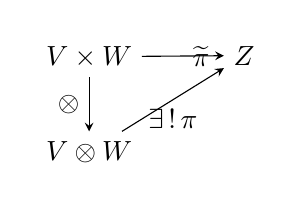
\begin{tikzpicture}
  \matrix (m) [matrix of math nodes, row sep=2em, column sep=3em, minimum width=1em]
  {
    V\times W  & Z  \\
    V\otimes W  &   \\ };
  \path[-stealth]
  (m-1-1) edge node [right] {$\widetilde{\pi}$} (m-1-2)
  edge node [left] { $\otimes$} (m-2-1)
  (m-2-1) edge node [below] {$\exists \, ! \, \pi$} (m-1-2);
\end{tikzpicture} 

is the universal property s.t. $\pi \otimes = \widetilde{\pi}$

Suppose bilinear $\widetilde{\pi} : V\times W \to Z$ s.t., \\
\quad \, $\forall \, $ bilinear $A: V\times W \to Y$, $\exists \, !$ linear $\widetilde{A} : Z \to Y$ s.t. 

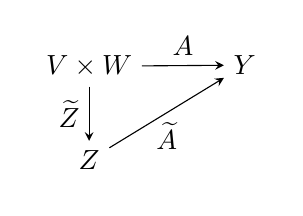
\begin{tikzpicture}
  \matrix (m) [matrix of math nodes, row sep=2em, column sep=3em, minimum width=1em]
  {
    V\times W  & Y  \\
    Z  &   \\ };
  \path[-stealth]
  (m-1-1) edge node [auto] {$A$} (m-1-2)
  edge node [left] { $\widetilde{Z}$} (m-2-1)
  (m-2-1) edge node [below] {$\widetilde{A}$} (m-1-2);
\end{tikzpicture} 

Consider 
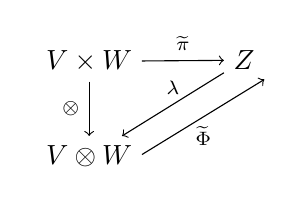
\begin{tikzpicture}
  \matrix (m) [matrix of math nodes, row sep=2em, column sep=3em, minimum width=1em]
  {
    V\times W  & Z  \\
    V\otimes W  &   \\ };
  \path[->,font=\scriptsize]
  (m-1-1) edge node [auto] {$\widetilde{\pi}$} (m-1-2)
  edge node [left] { $\otimes$} (m-2-1)
  (m-1-2) edge node [above] {$\lambda$} (m-2-1)
  (m-2-1.2) edge node [below] {$\widetilde{\Phi}$} (m-1-2.south east);
\end{tikzpicture} 

$\Phi \otimes = \widetilde{\pi}$ (by universal property) \\
\[
\Phi(v\otimes w) = \widetilde{\pi}(v,w)
\]
$\exists \, ! $ linear $\lambda : Z \to V\otimes W$ 
\[
\begin{aligned}
  & \lambda \circ \widetilde{\pi} = \otimes \\  
  & \lambda \otimes \widetilde{\pi}(v,w) = v\otimes w
\end{aligned}
\]

\[
\begin{aligned}
  & \Phi \lambda ( \widetilde{\pi}(v,w) ) = \Phi(v\otimes w) = \widetilde{\pi}(v,w) \\ 
  & \Phi \lambda = \text{id}_{Z} \\ 
  & \lambda \Phi(v\otimes w) = \lambda \widetilde{\pi}(v,w) = v\otimes w \\ 
  & \lambda \Phi = \text{id}_{V\otimes W}
\end{aligned}
\]
So $\Phi$ is an isomorphism between $Z, V\otimes W$.  As $\lambda $ is unique, so is $\Phi$



\problemhead{11-2}

tensor product of $U,V$ is vector space $U\otimes V$ with bilinear map $\begin{aligned} & \quad \\ 
  \otimes : & U \times V \to U\otimes V \\ 
  & (u,v) \mapsto u\otimes v \end{aligned}$ \\
with universal property with any vector space $W$.  

$K \cong k 1$ 

By bilinearity, 

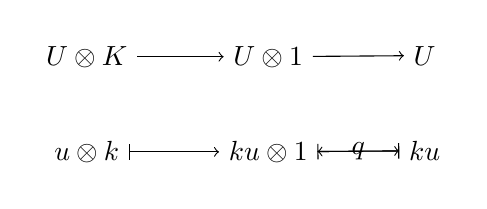
\begin{tikzpicture}
  \matrix (m) [matrix of math nodes, row sep=2em, column sep=3em]
  {
    U \otimes K  & U\otimes 1 & U  \\
    u\otimes k  & ku \otimes 1 & ku   \\ };
  \path[->]
  (m-1-1) edge node [auto] {$$} (m-1-2)
  (m-1-2) edge node [left] { $$} (m-1-3);
  \path[|->]
  (m-2-1) edge node [auto] {$$} (m-2-2)
  (m-2-2) edge node [above] {$$} (m-2-3);
  \path[|->]
  (m-2-3) edge node [bend right] {$q$} (m-2-2);
\end{tikzpicture} 

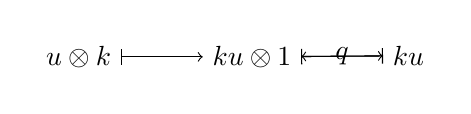
\begin{tikzpicture}
  \matrix (m) [matrix of math nodes, row sep=2em, column sep=3em]
  {
    u\otimes k  & ku \otimes 1 & ku   \\ };
%  \path[->]
%  (m-1-1) edge node [auto] {$$} (m-1-2)
%  (m-1-2) edge node [left] { $$} (m-1-3)
  \path[|->]
  (m-1-1) edge  (m-1-2)
  (m-1-2) edge  (m-1-3)
%  \path[|->]
  (m-1-3) edge node [bend left] {$q$} (m-1-2);
\end{tikzpicture} 

$q: U \to U\otimes 1$ \\
$u \mapsto u\otimes 1$

then $U\otimes K \simeq U$


\problemhead{11-3} $\begin{aligned} & \quad \\
  & U^* \times V \to \text{Hom}{(U,V)} \\
  & (u^*, v) \to ( u \to u^*(u), v) \end{aligned}$ induces a natural homomorphism (injective), $U^* \otimes V \to \text{Hom}{(U,V)}$ 
\begin{tikzpicture}
  \matrix (m) [matrix of math nodes, row sep=2em, column sep=3em]
  {
    U^* \otimes V  & \text{Hom}{(U,V)}    \\ };
%  \path[->]
%  (m-1-1) edge node [auto] {$$} (m-1-2)
%  (m-1-2) edge node [left] { $$} (m-1-3)
  \path[->]
  (m-1-1) edge  (m-1-2)
    edge node [auto] {$\otimes$} (m-2-1);
%  \path[|->]
    \path[dotted,->] 
  (m-2-1) edge  (m-1-2);
\end{tikzpicture} 

If $\text{dim}{U}, \, \text{dim}{V} < \infty$, 

for arbitrary $v_i \in V$, \, $\begin{aligned} & \quad \\
  & \sum_i e_i^* \otimes v_i \in U^* \otimes V \\
  & e_j \to e_i^*(e_j)v_i = v_j \end{aligned}$ 

$\sum_i e_i^* \otimes v_i$ corresponds to homomorphism $U\to V$ mapping $e_i \to v_i$ 

$U^* \otimes V \to \text{Hom}{(U,V)}$ surjective.  

$\text{dim}{U^* \otimes V} = \text{dim}{U^*} \text{dim}{V}$

isomorphism by dim. reason. 




\section{Differential Forms}
% 14differentialforms.tex
% Fund Science! & Help Ernest finish his Physics Research! : quantum super-A-polynomials - a thesis by Ernest Yeung
%                                               
% http://igg.me/at/ernestyalumni2014                                                                             
%                                                              
% Facebook     : ernestyalumni  
% github       : ernestyalumni                                                                     
% gmail        : ernestyalumni                                                                     
% google       : ernestyalumni                                                                                   
% linkedin     : ernestyalumni                                                                             
% tumblr       : ernestyalumni                                                               
% twitter      : ernestyalumni                                                             
% youtube      : ernestyalumni                                                                
% indiegogo    : ernestyalumni                                                                        
%
% Ernest Yeung was supported by Mr. and Mrs. C.W. Yeung, Prof. Robert A. Rosenstone, Michael Drown, Arvid Kingl, Mr. and Mrs. Valerie Cheng, and the Foundation for Polish Sciences, Warsaw University.                  


\subsection*{ The Geometry of Volume Measurement}

\subsection*{ The Algebra of Alternating Tensors }

\[
\begin{gathered}
  \text{Alt}: T^k(V) \to \Lambda^k(V) \\ 
  (\text{Alt}{T})(X_1 \dots X_k) = \frac{1}{k!} \sum_{ \sigma \in S_k} (\text{sgn}{\sigma}) T(X_{\sigma{(1)}} \dots X_{\sigma{(k)} } )
\end{gathered}
\]



\exercisehead{12.2} If $T$ alternating, by Exercise 12.1, $T(X_{\sigma(1)} \dots X_{\sigma{(k)} } ) = (\text{sgn}{\sigma})T(X_1 \dots X_k)$

\[
\begin{gathered}
  \frac{1}{k!} \sum_{\sigma \in S_k} (\text{sgn}{\sigma}) T(X_{\sigma{(1)} } \dots T_{\sigma{(k)} } ) = \frac{1}{k!} \sum_{\sigma \in S_k} (\text{sgn}{\sigma})(\text{sgn}{\sigma}) T(X_1 \dots X_k)  = \frac{1}{k!} \sum_{\sigma \in S_k} T(X_1 \dots X_k) = T(X_1 \dots X_k) \Longrightarrow \text{Alt}{T} = T
\end{gathered}
\]  



\subsubsection*{ Elementary Alternating Tensors }

\[
\begin{aligned}
  & I = (i_1 \dots i_k) \\ 
  & I_{\sigma} = (i_{\sigma(1)} \dots i_{\sigma(k)} ) \quad \quad \quad \sigma \in S_k
\end{aligned} 
\]
\[
\delta_I^{ \, \, J} = \begin{cases} \text{sgn}{\sigma} & \begin{gathered} \text{ if $I$ and $J$ has no repeated indices }\\ 
    \text{ and $J = I_{\sigma}$ for some $\sigma \in S_k$ } \end{gathered} \\
  0 & \begin{gathered} \text{ if $I$ and $J$ has repeated index } \\
    \text{ or $J \neq I_{\sigma} \quad \, \forall \, \sigma \in S_k $ } \end{gathered}
\end{cases}
\]
Let $V$ vector space, $(\epsilon^1 \dots \epsilon^n)$ basis for $V^*$ 

define covariant $k$-tensor $\epsilon^I$ by 
\[
\epsilon^I(x_1 \dots x_k) = \text{det}{ \left( \begin{matrix} \epsilon^{i_1}(X_1)  & \dots & \epsilon^{i_k}(X_k) \\ 
    \vdots & & \vdots \\ \epsilon^{i_k}(X_1) & \dots  & \epsilon^{i_k}(X_k) \end{matrix} \right) } = \text{det}{ \left( \begin{matrix} X_1^{\, i_1} & \dots & X_k^{\, i_k }  \\ \vdots &  & \vdots \\ X_1^{i_k} & \dots & X_k^{i_k} \end{matrix} \right) }
\]

denote sum over only increasing multi-indice
\[
\sum'_I T_I \epsilon^I = \sum_{ \lbrace I : 1\leq i_1 < \dots < i_k \leq n \rbrace } T_I \epsilon^I
\]

\begin{proposition}[12.5] for $k\leq n$

$\lbrace \epsilon =  \epsilon^I : I \text{ an increasing multi-index of length $k$ } \rbrace$ is a basis for $\Lambda^k(V)$ 
\end{proposition}
\[
\Longrightarrow \text{dim}{ \Lambda^k(V) }= \binom{n}{k} 
\]



\begin{lemma}{12.6} $\omega \in \Lambda^n(V)$ 

If linear $T: V \to V$, $X_1 \dots X_n \in V$ 
\begin{equation}
  \omega(TX_1 \dots TX_n) = \text{det}{T} \omega(X_1 \dots X_n) \quad \quad \quad (12.2) 
\end{equation}

\end{lemma}

\begin{proof}
  By Prop. 12.5, $\mathcal{E} = \lbrace \epsilon^I | I \text{ increasing multi-index of length $k$ } \rbrace \text{ basis for $\Lambda^k(V)$ }$
\[
\omega = c\epsilon^{1 \dots n} \quad \quad \quad \binom{n}{n} =1 
\]
By multilinearity of $\omega(TX_1 \dots TX_n)$ and $(\text{det}{T}) \omega(X_1 \dots X_n)$, it suffices to verify it in special case
\[
X_i = E_i, \quad i = 1 \dots n
\]
\end{proof}

\[
\begin{gathered}
  \text{det}{T} \omega(X_1 \dots X_n) = \text{det}{T} c\epsilon^{1\dots n}(E_1 \dots E_n) = c\text{det}{T} \\ 
  \omega(TE_1 \dots TE_n) = c\epsilon^{1\dots n}(T_1 \dots T_n) = c\text{det}{( \epsilon^j(T_i)) } = c\text{det}{ (\epsilon^j(T_i^{ \, \, k}e_k) ) } = c\text{det}{T_i^{\, \, j}} \\ 
\text{ where, recall } \epsilon^I(X_1 \dots X_k) = \text{det}{X_j}^{ \, \, i_k}
\end{gathered}
\]




\subsubsection*{ The Wedge Product }

\begin{lemma}[14.10]
  \begin{equation}
    \epsilon^I \wedge \epsilon^J = \epsilon^{IJ}
\end{equation}
\end{lemma}

\subsection*{ Differential Forms on Manifolds }

Recall $T^k T^*M$ bundle of covariant $k$-tensors on $M$ \\
\quad alternating tensors $\Lambda^k T^*M \subset T^k T^*M$ \\

\[
\Lambda^k T^*M = \coprod_{ p \in M} \Lambda^k{ ( T^*_p M )}
\]

\exercisehead{14.14} 

$\Lambda^k T^*M$ smooth subbundle of $T^kT^*M$

EY : 20140501 EY? ???

\hrulefill

denote section

\[
\Omega^k{ (M) } = \Gamma{ (\Lambda^k T^* M ) }
\]



in any smooth chart, $k$ form $\omega$ can be written locally as 
\[
\omega = \sum_I' \omega_I dx^{i_1} \wedge \dots \wedge dx^{i_k} = \sum_I' \omega_I dx^I
\]

%By Lemma 12.4(c)
By Lemma 14.7(c)
\[
dx^{i_1} \wedge \dots \wedge dx^{i_k} \left( \frac{ \partial }{ \partial x^{j_1} } \dots \frac{ \partial }{ \partial x^{j_k} } \right) = \delta^I_{\, \, J}
\]
component functions $\omega^I$ of $\omega$ determined by 
\[
\omega^I = \omega\left( \frac{ \partial }{ \partial x^{i_1} } \dots \frac{ \partial }{ \partial x^{i_k} } \right)
\]

\[
(F^* \omega)(v_1 \dots v_k) = \omega( dF(v_1) \dots dF(v_k) )
\]

\[
\begin{aligned}
  & e_i \in TM \\ 
  & f_j \in TN
\end{aligned}
\]
\[
F(x) = F^j(x) = y^j( x^i)
\]

\[
\begin{aligned}
  & F_*(v) = w = w^j f_j \\ 
  & F_*(v) = vF = v^i \frac{ \partial F^j}{ \partial x^i } f_j
\end{aligned} \quad \quad \, \Longrightarrow w^j = v^i \frac{ \partial^j F}{ \partial x^i}
\]

\[
(F^*\omega)(v_1 \dots v_k)  = \omega(F_*v_1 \dots F*v_k) = \omega(v_1 F \dots v_k F)
\]
\[
(F^*\omega) = (F^* \omega)_{ \underline{I}} dx^{ \underline{I}}
\]
\[
(F^* \omega) e_I = (F^* \omega)_{\underline{I}}
\]
\[
\omega(dF(e_I)) = \omega(F_* e_I) = \omega_{\underline{J}}(DF)^{\underline{J}}_{ \, \, I }
\]

\[
\begin{gathered}
  F_*e_I = (F_* e_I)^J f_J = (DF)^J_{ \, \, I } f_J \\ 
 (F^* \omega)_{\underline{I}} = \omega_{\underline{J}} (DF)^{\underline{J}}_{ \, \, I } 
\end{gathered}
\]



\begin{lemma}[14.16]
\begin{enumerate}
  \item[(a)] $F^* : \Omega^k(N) \to \Omega^k(M)$ linear over $\mathbb{R}$ 
\item[(b)] $F^*(\omega \wedge \eta) = (F^* \omega) \wedge (F^* \eta)$
\item[(c)] in any smooth chart 
\[
F^*( \omega_{\underline{I}} dy^{\underline{I}} ) = (\omega_{\underline{I}} F) ( dy^{ \underline{I}} F)
\]
\end{enumerate}
\end{lemma}



\exercisehead{14.17}

$\omega, \eta \in \Omega^k(N)$ \quad \quad \, $\begin{aligned} & \quad \\
  & F^* \omega = \alpha \\
  & F^* \eta = \beta \end{aligned}$


\[
\begin{aligned}
  & (F^* \omega)  = (F^* \omega)_{\underline{I}} e^{\underline{I}} = \alpha_{\underline{I}} e^{ \underline{I}} \\ 
  &  (F^* \eta) = (F^* \eta)_{\underline{J}} e^{ \underline{J}} = \beta_{\underline{J}} e^{\underline{J}}
\end{aligned}
\]
\begin{enumerate}
\item[(a)] \[
\begin{gathered}
  \alpha + \beta  = F^* \omega + F^*\eta = (\alpha_{\underline{I}} + \beta_{\underline{I}} ) dx^{\underline{I}} = (\omega(dF(e_{\underline{I}} ) ) + \eta( dF(e_{\underline{I}})) )dx^{\underline{I}} = (\omega+ \eta) dF(e_I) dx^{\underline{I}} = F^*(\omega + \eta)(e_{\underline{I}})dx^{\underline{I}} = \\
  = F^*(\omega+ \eta)
\end{gathered}
\]
\[
F^*c\omega = c \omega DF = c F^*\omega
\]
\item[(b)] \[
\begin{aligned}
  & \alpha \wedge \eta = \alpha_{\underline{I}} \beta_{\underline{J}} e^{ \underline{I}} \wedge e^{ \underline{J}} \\
  & \alpha \wedge \eta = (\alpha \wedge \eta)_{\underline{K}} e^{ \underline{K}}  \\
  & (\alpha \wedge \eta)_{\underline{K}} = \alpha_{\underline{I}} \beta_{\underline{J}} \delta^{ \underline{I} \underline{J}}_{ \underline{K}}  \\
& \omega \wedge \eta = \omega_{\underline{I}} f^{\underline{I}} \wedge \eta_{\underline{J}} f^{\underline{J}} = \omega_{\underline{I}} \eta_{\underline{J}} f^{\underline{I}} \wedge f^{\underline{J}}
\end{aligned}
\]

\[
F^*(\omega \wedge \eta) e_{\underline{K}} = (\omega \wedge \eta) DF e_{\wedge{K}} = \omega_{\underline{I}} \eta_{\underline{J}} f^{ \underline{I}} \wedge f^{\underline{J}} DF^K_{ \underline{K}} f_L = \omega_{\underline{I}} \eta_{\underline{J}} DF^L_{\underline{K}} \delta^{ \underline{I} \underline{J}}_L = \omega_{\underline{I}} \eta_{\underline{J}} DF^{ \underline{I}\underline{J}}_{\underline{K}}
\]
In the last equality, $\underline{I} \underline{J}$ in $DF^{\underline{I}\underline{J}}_{\underline{K}}$ is some permutation of $\underline{I}\underline{J}$


\[
\begin{gathered}
  (F^*\omega) \wedge (F^* \eta) e_{\underline{K}} = \omega_{\underline{J}} DF^{\underline{J}}_{\underline{I}} \eta_{\underline{L}} DF^{\underline{L}}_{ \underline{M}} (e^{\underline{I}} \wedge e^{\underline{M}} ) e_{\underline{K}} = \omega_{\underline{J}} \eta_{\underline{L}} DF^{\underline{J}}_{\underline{I}} DF^{\underline{L}}_{\underline{M}} \delta^{\underline{I}\underline{M}}_{\underline{K}}     = \omega_{\underline{I}} \eta_{\underline{J}} DF^{\underline{I}}_{\underline{L}} DF^{\underline{J}}_{\underline{M}} \delta^{\underline{L} \underline{M}}_{\underline{K}}
\end{gathered}
\]
\item[(c)]
\end{enumerate}


\subsection*{ Exterior Derivatives }

$\forall \, $ manifold, $\exists \, $ differential operator
\[
d: \mathcal{A}^k(M) \to \mathcal{A}^{k+1}(M)
\]
s.t. $d(d\omega ) =0 \quad \, \forall \, \omega$

necessary: if smooth $k$-form $\omega = d\eta$, some $(k-1)$ form $\eta$, then $d\omega =0$

in coordinates
\begin{equation}
  d \left( \sum_J' \omega_J dx^J \right) = \sum_J' d\omega_J \wedge dx^J \quad \quad \quad (12.15)
\end{equation}

\begin{equation}
  d\left( \sum_J' \omega_J dx^{j_1} \wedge \dots \wedge dx^{j_k} \right) = \sum_J' \sum_i \frac{ \partial \omega_J}{ \partial x^i} dx^i \wedge dx^{j_1} \wedge \dots \wedge dx^{j_k} \quad \quad \quad (12.16)
\end{equation}


\begin{theorem}[12.14] (The Exterior Derivative) 

$\forall \, $ smooth $M$, $\exists \, !$ linear $d: \mathcal{A}^k(M) \to \mathcal{A}^{k+1}(M)$ s.t. 
\begin{enumerate}
\item[(i)] if $f$ smooth, $f\in \mathbb{R}$ (0-form), then differential $df$, defined 
\[
df(X) = Xf
\]
\item[(ii)] if $\begin{aligned} & \quad \\ & \omega \in \mathcal{A}^k(M) \\ & \eta \in \mathcal{A}^l(M) \end{aligned}$, then $d(\omega \wedge \eta) = d\omega \wedge \eta + (-1)^k \omega \wedge d\eta $
\item[(iii)] $d^2 =0$
\end{enumerate}
\begin{enumerate}
  \item[(a)] $\forall \, $ smooth coordinate chart, $d$ given by (12.15) 
  \item[(b)] $d$ local; if $\omega = \omega'$ on open $U \subset M$, then $d\omega = d\omega'$ on $U$
  \item[(c)] $d$ commutes with restriction if $U \subset M$ any open set
    \begin{equation}
      d(\left. \omega \right|_U ) = \left. d(\omega ) \right|_U \quad \quad \quad (12.17)
    \end{equation}
\end{enumerate}
\end{theorem}


\begin{proof}
  Suppose $M$ covered by a single chart.  

define $d$ by (12.15) 
\[
d\left( \sum_J' \omega_J dx^J \right) = \sum_J' d\omega_J \wedge dx^J \quad \quad \quad (12.15) 
\]
\[
df(X) = df(X^i e_i ) = X^i f(e_i)
\]

$d$ linear, (i) satisfied.  

Consider $\begin{aligned} & \quad \\ & \omega = fdx^I \\ & \eta = gdx^J \end{aligned}$ 
\[
\begin{gathered}
  d(\omega \wedge \eta) = d((fdx^I ) \wedge (g dx^J)) = d(fg dx^I \wedge dx^J) = (gdf + fdg) \wedge dx^I \wedge dx^J = \\
   = (df \wedge dx^I) \wedge (gdx^J) + (-1)^k( fdx^I ) \wedge (dg \wedge dx^J) = d\omega \wedge \eta + (-1)^k \omega \wedge d\eta
\end{gathered}
\]
(ii) proved.  

0-form

\[
\begin{gathered}
  d(df) = d \left( \frac{ \partial f}{ \partial x^j} dx^j \right) = \frac{ \partial^2 f}{ \partial x^i \partial x^j} dx^i \wedge dx^j = \sum_{ i < j } \partial^2_{ij} f dx^i \wedge dx^j + \sum_{j < k } \partial^2_{ij} f dx^j \wedge dx^i = \\
   = \sum_{i < j } \left( \frac{ \partial^2 f}{ \partial x^i \partial x^j} - \frac{ \partial^2 f}{ \partial x^j \partial x^i } \right) dx^i \wedge dx^j = 0 
\end{gathered}
\]

for $k$-form, use $k=0$ case, (ii)

\[
\begin{gathered}
  d(d\omega) = d\left( \sum_J' d\omega_J \wedge dx^{j_1} \wedge \dots \wedge dx^{j_k} \right) = \\
  = \sum_J' d(d \omega_J) \wedge dx^{j_1} \wedge \dots \wedge dx^{j_k} + \sum_J' \sum_{i=1}^k (-1)^i d\omega_J \wedge dx^{j_1} \wedge \dots \wedge d(dx^{j_i}) \wedge \dots \wedge dx^{j_k} = 0 
\end{gathered}
\]

from (12.17), $d( \left. \omega \right|_U ) = \left. (d\omega ) \right|_U$
\[
\left. (d_U \omega) \right|_{UU'} = d_{UU'} \omega = \left. (d_{U'} \omega) \right|_{UU'}
\]
Suppose $\exists \, $ another operator $\widetilde{d} : \mathcal{A}^k(M) \to \mathcal{A}^{k+1}(M)$

$\eta = \omega - \omega'$, let $p\in U$. 

Let $\varphi \in \mathcal{C}^{\infty}(M)$ smooth bump function, $\varphi =1$ in neighborhood of $p$, supported in $U$.  

Then $\varphi \eta =0 $ in $M$, so 
\[
 0 = \widetilde{d}(\varphi \eta)_p = d\varphi_p \wedge \eta_p  + \varphi(p) \widetilde{d}\eta_p = \widetilde{d}\eta_p
\]
because $\varphi \equiv 1$ in neighborhood of $p$

$p$ arbitrary, so $d\eta = 0$ on $U$.  $d\omega = d\omega'$ (locality)

\end{proof}

Antiderivation of degree $g \in \mathbb{Z}$ on $\mathbb{Z}$-graded $\mathbb{R}$-algebra $A = \bigoplus_{k \in \mathbb{Z}} A_k $ in $\mathbb{R}$-linear $D: A \to A$
\[
D(A_k) = A_{k +g}
\]

s.t.
\[
D(a_k a_l) = (Da_k) a_l + (-1)^k a_k(Da_l) \quad \quad a_k \in \mathcal{A}_k, \, a_l \in A_l
\]

Example 12.15.  
\[
\omega = P dx + Q dy + R dz
\]
Recall 
\[
d\left( \sum'_J \omega_J dx^J \right) = \sum_J' d\omega_J \wedge dx^J
\]

\[
\begin{gathered}
  d\omega  = dP \wedge dx + dQ \wedge dy + dR \wedge dz = \\
   =\left( \frac{ \partial P }{ \partial x} dx + \frac{ \partial P }{ \partial y} dy + \frac{ \partial P }{ \partial z} dz \right) \wedge dx + \left( \frac{ \partial Q}{ \partial x} dx + \frac{ \partial Q}{ \partial y} dy + \frac{ \partial Q}{ \partial dz }dz \right) \wedge dy + \left( \frac{ \partial R}{ \partial x} dx + \frac{ \partial R}{ \partial y} dy + \frac{ \partial R}{ \partial z} dz \right) \wedge dz  \\
= \left( \frac{ \partial Q}{ \partial x} - \frac{ \partial P }{ \partial y} \right) dx \wedge dy + \left( \frac{ \partial R}{ \partial x} - \frac{ \partial P }{ \partial z} \right) dx \wedge dz + \left( \frac{ \partial R}{ \partial y} - \frac{ \partial Q}{ \partial z } \right) dy \wedge dz
\end{gathered}
\]


\subsubsection*{An Invariant Formula for the Exterior Derivative}

\begin{proposition}[14.29 (Exterior Derivative of a 1-Form)]
  \begin{equation}
    d\omega(X,Y) = X(\omega(Y)) - Y(\omega(X)) - \omega([X,Y])
\end{equation}
\end{proposition}

\begin{proof}
  $\forall \, \omega \in \Omega^1(M)$, $\omega = udv$ for some $u,v \in C^{\infty}(M)$
  \[
\begin{aligned}
  & d\omega(X,Y) = d(udv)(X,Y) = du \wedge dv(X,Y) = du(X) dv(Y) - dv(X)du(Y) = X(u)Y(v) - X(v)Y(u) \\ 
  & X(udv(Y))= X(uY(v)) = X(u)Y(v) + uXY(v) \\
  & Y(udv(X))= Y(uX(v)) = Y(u)X(v) + uYX(v) \\
  & udv([X,Y]) = uXYv - uYXv \\
  & \Longrightarrow d\omega(X,Y) = X(\omega(Y)) - Y(\omega(X)) - \omega([X,Y])
\end{aligned}
\]
\end{proof}

\begin{proposition}[14.30]
  Let smooth manifold $M$ of $\text{dim}M = n$, \\
  Let $(E_i)$ smooth local frame for $M$, let $(\epsilon^i)$ dual coframe. \\
  Let $d\epsilon^i = \sum_{j<k} b^i_{jk} \epsilon^j \wedge \epsilon^k $ \\
  \phantom{Let }$[E_j,E_k] = c^i_{jk} E_i$

Then $b^i_{jk} = -c^i_{jk}$
\end{proposition}

Proof is Exercise 14.31.  

\exercisehead{14.31}

\begin{proof}
  Assume $j <k$ without loss of generality.  
  \[
\begin{gathered}
  d\epsilon^i(E_j,E_k) = \sum_{j' < k'} b^i_{j'k'}(\delta^{j'}_j \delta^{k'}_k - \delta^{j'}_k \delta^{k'}_j = b^i_{jk} = E_j \delta^i_k - E_k \delta^i_j - c^i_{jk} \\
  \Longrightarrow b^i_{jk} = -c^i_{jk}
\end{gathered}
\]
\end{proof}

\subsubsection*{Lie Derivatives of Differential Forms}


\begin{proposition}[14.33]
  Suppose $M$ smooth manifold, $V \in \mathfrak{X}(M)$, $\omega, \eta \in \Omega^*(M)$ 
\[
\mathcal{L}_V(\omega \wedge \eta) = (\mathcal{L}_V \omega) \wedge \eta + \omega \wedge (\mathcal{L}_V \eta)
\]
\end{proposition}

\begin{theorem}[14.35] (Cartan's Magic Formula) 

\[
\mathcal{L}_V \omega = V \righthalfcup (d\omega) + d(V\righthalfcup \omega) = 
\]

EY

\[
= i_V(d\omega) + d(i_V\omega)
\]
\end{theorem}

\begin{corollary}[14.36] (The Lie Derivative Commutes with $d$)
\[
\mathcal{L}_V(d\omega) = d(\mathcal{L}_V\omega)
\]
\end{corollary}



\section{Orientations}
\subsection*{ Orientations of Vector Spaces }

\exercisehead{13.1} 
\[
\begin{gathered}
  (E_1 \dots E_n) \sim (E_1 \dots E_n) \\ 
  E_i = \delta_i^{\, \, j } E_j \\ 
  \text{det}{ (\delta_i^{\, \, j} )} = 1 
\end{gathered}
\]

If $E_i = B_i^{\, \, j} \widetilde{E}_j$, \, $\text{det}{B_i^{\, \, j }} >0$,  
% \[
%(B^{-1})_i^{\, \, k} E_k = (B^{-1})_i^{\, \, k } B_k^{\, \, j} \widetilde{E}_j = E_
% #\]

$\text{det}{(BB^{-1})} = \text{det}{B} \text{det}{B^{-1}} = 1$.  $\text{det}{B^{-1}} >0$ since $\text{det}{B} >0$.  

If $E_i = B_i^{\, \, j} \widetilde{E}_j$  
\[
\begin{aligned}
  & \widetilde{ \widetilde{E}}_i = A_i^{\, \, j} E_j \\ 
  & \widetilde{ \widetilde{E}}_i = A_i^{\, \, k } B_k^{\, \, j} \widetilde{E}_j \quad \quad \text{det}{AB} = \text{det}{A} \text{det}{B} >0
\end{aligned}
\]
So it's an equivalence relation and since $\text{det}{B} \neq 0$, $\text{det}{B} >0$ or $\text{det}{B} <0$ and as above there are only 2 equivalence classes; $\text{det}{A} \gtrless 0$

\subsection*{ Orientations of Manifolds }

lcaol frame $(E_i)$ for $M$ is (positively) oriented if $(\left. E_1 \right|_p \dots \left. E_n \right|_p)$ positively oriented basis for $T_pM$.  $\forall \, p \in U$  

cont. if $\forall \, p \in M$, $p\in $ domain of oriented local frame.  

orientation of $M$ is cont., pointwise orientation.  

$M$ orinetable if $\exists \, $ orientation to $M$

\exercisehead{13.2}  connected domain $U$.  Consider some $\Omega \in \Lambda^m(V)$,  consider 
\[
\begin{aligned}
  & U \to \mathbb{R} \\ 
  & p \mapsto ( \left. E_1 \right|_p \dots \left. E_n \right|_p ) \mapsto \Omega( \left. E_1 \right|_p \dots \left. E_n \right|_p ) = \text{det}{ ( \left.  \epsilon^i(E_j) \right|_p ) }
\end{aligned}
\]

$\text{det}$ cont. function s.t. $\text{det} = \begin{cases} +1 \\ -1 \end{cases}$ on $U$.  $U$ connected so $\forall \, $ cont. functions from $X$ to $\lbrace 0, 1 \rbrace$ or, the same, $\lbrace 1 , -1 \rbrace$, constant.  \\
So $\Omega( \left. E_1 \right|_p \dots \left. E_n \right|_p ) = \text{det}{ ( \left. \epsilon^i (E_j) \right|_p )}$ constant on $U$, otherwise $U$ separated.  

\begin{proposition}[13.4] 
$\text{dim}{M} = m \geq 1$ 

$\forall \, m$-form $\Omega$ on $M$, $\Omega\neq 0$ determines a unique orientation of $M$ s.t. $\Omega$ positively oriented $\forall \, p \in M$, \\
Conversely, if $M$ given orientation, then $\exists \, $ smooth $m$-form $\Omega$ on $M$ that's positively oriented $\forall \, p \in M$
\end{proposition}

$F:M \to N$ local diffeomorphism.  

$\forall \, p \in M$, $\exists \, (U, \varphi)$ chart and consider $U_F \subset U$ s.t. $F(U_F)$ open, $\left. F\right|_{U_F} : U_F \to F(U_F)$ diffeomorphism.  

For $F(p) \in N$, $\exists \, (V, \psi)$ chart and consider $F(U_F) \cap V$

$\psi F\varphi^{-1}(x^1 \dots x^m) = F^j(x^1 \dots x^m)$ \quad \quad $\text{det}{(\partial_i F^j)} >0$ suppose.  


\subsection*{The Orientation Covering}

\subsection*{Orientations of Hypersurfaces }

interior multiplication or contraction with $X$
\[
i_X\omega(Y_1 \dots Y_{k-1}) = \omega(X,Y_1 \dots Y_{k-1})
\]
$i_X \omega$ obtained by inserting $X$ into the first slot.

Notation $X \righthalfcup \omega = i_X \omega$









Suppose $M$ smooth manifold \\
\phantom{Suppose} $S\subset M$ submanifolds (immersed or embedded)

vector field along $S$ is cont. $N: S \to TM$ s.t. $N_p \in T_pM$ \quad $\forall \, p \in S$

(Note difference between vector field along $S$ and vector field on $S$, s.t. $N_p \in T_pS \, \forall \, p$)

$N_p \in T_pM$, $p\in S$ transverse to $S$ if $T_pM$ spanned by $N_p, T_pS$

Similarly, vector field $N$ along $S$ transverse to $S$ if $N_p$ transverse to $S$, \, $\forall \, p \in S$




\begin{proposition}[15.21, 13.12 in previous version] Suppose $M$ oriented smooth $m$-manifold \\
\phantom{Proposition 13.12 Suppose  } $S$ immersed hypersurface in $M$.  \\
\phantom{Proposition 13.12 Suppose  } $N$ transverse vector field along $S$.  

Then $S$ has unique orientation s.t. $\forall \, p \in S$, $(E_1 \dots E_{n-1})$ oriented basis for $T_pS$ iff $(N_p, E_1 \dots E_{n-1})$ oriented basis for $T_pM$

If $\Omega$ orientation form for $M$, \\
then $\left. (N \righthalfcup \Omega) \right|_S \equiv \left. i_N\Omega \right|_S $ orientation form for $S$ with respect to this orientation.  
\end{proposition}

Recall that smooth hypersurface $S$ is $S\subseteq M$ equipped with $i: S \hookrightarrow M$, smooth immersion, i.e. $Di$ injective.  

Now orientation form $\omega = dN_p \wedge dE_1 \wedge \dots \wedge dE_{n-1}$, then \\
$i_{N_p} \omega  =dE_1 \wedge \dots \wedge dE_{n-1}$
\[
i^*_S (i_{N_p}\omega) = i^*_S (dE_1 \wedge \dots \wedge dE_{n-1}) = i^*_S(dE_1) \wedge \dots \wedge i^*_S(dE_{n-1}) = d(i^*_SE_1) \wedge \dots \wedge d(i_S^*E_{n-1})
\]



\begin{proof} Let $\Omega$ \\
\phantom{proof Let } $\omega  = \left. (N \righthalfcup \Omega) \right|_S$ $m-1$ form.  

$(E_1 \dots E_{n-1}) $ basis for $T_pS$ \\
$N$ transverse to $S$ implies $(N_p, E_1 \dots E_{n-1})$ basis for $T_pM$.  

$\Omega$ orientation form so $\Omega$ nonvanishing.  
\[
\omega_p(E_1 \dots E_{n-1}) = \Omega_p(N_p, E_1 \dots E_{n-1}) \neq 0
\]
since $\omega_p(E_1 \dots E_{n-1}) >0$ iff $\Omega_p(N_p, E_1 \dots E_n) >0$,  \\
orientation determined by $\omega$ is the 1 defined in the statement of the proposition.  

\end{proof}



\section{Integration on Manifolds}
% 16integrationonmanifolds.tex
% Fund Science! & Help Ernest finish his Physics Research! : quantum super-A-polynomials - a thesis by Ernest Yeung
%                                               
% http://igg.me/at/ernestyalumni2014                                                                             
%                                                              
% Facebook     : ernestyalumni  
% github       : ernestyalumni                                                                     
% gmail        : ernestyalumni                                                                     
% google       : ernestyalumni                                                                                   
% linkedin     : ernestyalumni                                                                             
% tumblr       : ernestyalumni                                                               
% twitter      : ernestyalumni                                                             
% youtube      : ernestyalumni                                                                
% indiegogo    : ernestyalumni                                                                        
%
% Ernest Yeung was supported by Mr. and Mrs. C.W. Yeung, Prof. Robert A. Rosenstone, Michael Drown, Arvid Kingl, Mr. and Mrs. Valerie Cheng, and the Foundation for Polish Sciences, Warsaw University.                  


\subsection*{Integration of Functions on Riemannian Manifolds}

\begin{proposition}[16.28]
  $(M,g)$ oriented Riemannian manifold with or without $\partial$ \\
Suppose $f$ compactly supported cont. on $M$, $f\in \mathbb{R}$, $f\geq 0$ \\
Then $\int_M f dV_g \geq 0$ \\
\phantom{Then } $\int_M f dV_g = 0$ iff $f=0$
\end{proposition}

\begin{proof}
  If $f$ supported in \\
\quad \, domain of single oriented smooth chart $(U,\varphi)$  \\

By Prop. 15.31


\[
\int_M f dV_g = \int_{ \varphi{(U)}} f(x) \sqrt{ \text{det}{ (g_{ij} ) } } dx^1 \dots dx^n \geq 0
\]




\end{proof}

\exercisehead{16.29} given oriented Riemannian manifold $(M,g)$ \\
\quad compact supported cont. $f: M \to \mathbb{R}$ \\

Then if $f$ supported in \\
\phantom{Then } domain of single oriented smooth chart $(U,\varphi)$ 

\[
\left| \int_M f dV_g \right| = \left| \int_{ \varphi{ (U)} } f(x) \sqrt{ \text{det}{ (g_{ij} )} } dx^1 \dots dx^n \right| \geq \int_{\varphi{ (U)} } |f(x) | \sqrt{ \text{det}{ (g_{ij})} } dx^1 \dots dx^n = \int_M |f| dV_g
\]

where inequality above is from some thm. in calculus.  

\hrulefill

\subsection*{The Divergence Theorem}


\begin{equation}
  \begin{aligned}
    & * : C^{\infty}{ (M)} \to \Omega^n{ (N) } \\  
    & * f = f dV_g 
\end{aligned} \quad \quad \quad \, (16.10)
\end{equation}
smooth bundle isomorphism 

EY : 20140501 smooth bundle isomorphism? 

smooth bundle isomorphism

\[
\begin{aligned}
  & \beta : \mathfrak{X}{(M)} \to \Omega^{n-1}{ (M) } \\ 
  &  \beta(X) = X \righthalfcup dV_g
\end{aligned}
\]

technical lemma
\begin{lemma}[16.30]
  $(M,g)$ oriented Riemannian manifold with or without $\partial$ \\
  Suppose $S \subseteq M$ immersed hypersurface with orientation by \\
\phantom{Suppose } unit normal vector field $N$ and \\
\phantom{Suppose } $\widetilde{g}$ induced metric on $S$ \\

If $X$ any vector field along $S$, 

\begin{equation}
  i^*_S{ (\beta{ (X)} )}  = \langle X, N \rangle_g dV_{\widetilde{g}} \quad \quad \quad \, (16.12)
\end{equation}



\end{lemma}

\begin{proof}
Define vector fields $X^T$, $X^{\perp}$ along $S$

\[
\begin{aligned}
&  X^{\perp} = \langle X, N\rangle_g N \\ 
&  X^T =  X - X^{\perp}
\end{aligned}
\]

\[
\beta(X) = X \righthalfcup dV_g = X^{\perp} \righthalfcup dV_g + X^T \righthalfcup dV_g
\]

pull back to $S$

Prop. 15.32


\[
i^*_S{ (X^{\perp} \righthalfcup dV_g) }  = \langle X, N \rangle_g i^*_S{ (N \righthalfcup dV_g) } = \langle X, N \rangle_g dV_{ \widetilde{g}}
\]

If $X_1 \dots X_{n-1}$ any vectors tangent to $S$

\[
(X^T \righthalfcup dV_g){ (X_1 \dots X_{n-1} ) } = dV_g{ (X^T, X_1 \dots X_{n-1} ) } = 0 
\]



\end{proof}




\section{De Rham Cohomology}

$d\omega = 0$ closed \\
$\omega = d\eta$ exact.   \\

Prop. 6.24 smooth 1-form conservative iff exact.

\subsection*{ The de Rham Cohomology Groups}

closed 1-form 
\begin{equation}
\omega = \frac{ x dy - y dx}{ x^2 + y^2 }  \quad \quad \quad \, (15.1)
\end{equation}

Suppose 
\[
\begin{gathered}
\begin{aligned}
  x & = r\cos{\theta} \\ 
  y & = r s_{\theta} 
\end{aligned} \quad \quad \, \begin{aligned}
  dx & = c_{\theta}dr + -r s_{\theta} d\theta \\ 
  dy & = s_{\theta} dr + rc_{\theta} d\theta
\end{aligned} \\
d\alpha = \omega = \frac{ x dy - y dx}{ x^2 + y^2 } = \frac{ x}{ x^2 + y^2 } - \frac{y}{x^2 + y^2} dx = \frac{1}{r} c_{\theta} ( s_{\theta} dr + rc_{\theta} d\theta ) - \frac{s_{\theta}}{r} ( c_{\theta} dr - rs_{\theta} d\theta) = d\theta 
\end{gathered}
\]

$M$ smooth manifold

$d: \mathcal{A}^p(M) \to \mathcal{A}^{p+1}(M)$ linear, $\text{ker}$, $\text{im}$ linear subspaces.  \\
$\mathcal{Z}^p(M) = \text{ker}{ [ d : \mathcal{A}^p(M) \to \mathcal{A}^{p+1}(M)] } = \lbrace \text{ closed $p$-forms on $M$ } \rbrace$ \\
$\mathcal{B}^p(M) = \text{im}{ [ d: \mathcal{A}^{p-1}(M) \to \mathcal{A}^p(M)]} = \lbrace \text{ exact $p$-forms on $M$ } \rbrace$


By convention, $\mathcal{A}^p(M)$ zero vector space, $p < 0$ or $p>n = \text{dim}{M}$

e.g.

\[
\begin{aligned}
  \mathcal{B}^0(M)=0 \\ 
  \mathcal{Z}^n(M) = \mathcal{A}^n(M)
\end{aligned}
\]

$d^2=0$ so \\
$\forall \, $ exact form closed.  $\mathcal{B}^p(M) \subset \mathcal{Z}^p(m)$

\[
H^p_{dR}(M) = \frac{\mathcal{Z}^p(M)}{ \mathcal{B}^p(M) }
\]


\subsection*{Homotopy Invariance}

\begin{lemma}[15.4] (Existence of a Homotopy Operator)
  $\forall \, $ smooth manifold $M$, $\exists \, $ homotopy operator $\mathcal{i}_0^*$, $\mathcal{i}^*_1$
\end{lemma}

\begin{proof} $\forall \, p$, define linear $h: \mathcal{A}^p(M\times I) \to \mathcal{A}^{p -1}(M)$ s.t. 
\begin{equation}
h(d\omega ) + d(h \omega) = \mathcal{i}^*_1 \omega - \mathcal{i}_0^*\omega  \quad \quad \, (15.5)
\end{equation}


define $h\omega = \int_0^1 \left( \frac{ \partial }{\partial t} \lrcorner \omega \right) dt$


$h \omega$ \, $(p-1)$ form on $M$ whose action on $X_1 \dots X_{p-1} \in T_qM$ is 
\[
(h\omega)_q(X_1  \dots X_{p-1}) = \int_0^1 \left( \frac{ \partial }{ \partial t} \lrcorner \omega(q,t) \right)(X_1 \dots X_{p-1} ) dt = \int_0^1 \omega_{(q,t)}\left( \frac{ \partial}{\partial t}, X_1 \dots X_{p-1} \right) dt 
\]

choose smooth local coordinates $(x^i)$ on $M$.

Consider separately $\begin{aligned} & \quad \\ 
  \omega  & = f(x,t) dt \wedge dx^{i_1} \wedge \dots \wedge dx^{i_{p-1} } \\  
  \omega & = f(x,t) dx^{i_1} \wedge \dots \wedge dx^{i_p } \end{aligned}$


\end{proof}

%\section{The de Rham Theorem}

\section{Distributions and Foliations}
% 19DistributionsaFoliations.tex
% Fund Science! & Help Ernest finish his Physics Research! : quantum super-A-polynomials - a thesis by Ernest Yeung
%                                               
% http://igg.me/at/ernestyalumni2014                                                                             
%                                                              
% Facebook     : ernestyalumni  
% github       : ernestyalumni                                                                     
% gmail        : ernestyalumni                                                                     
% google       : ernestyalumni                                                                                   
% linkedin     : ernestyalumni                                                                             
% tumblr       : ernestyalumni                                                               
% twitter      : ernestyalumni                                                             
% youtube      : ernestyalumni                                                                
% indiegogo    : ernestyalumni                                                                        
%
% Ernest Yeung was supported by Mr. and Mrs. C.W. Yeung, Prof. Robert A. Rosenstone, Michael Drown, Arvid Kingl, Mr. and Mrs. Valerie Cheng, and the Foundation for Polish Sciences, Warsaw University.                  
%
%These notes are open-source, governed by the Creative Common license.  Use of these notes is governed by the Caltech Honor Code: ``No member of the Caltech community shall take unfair advantage of any other member of the Caltech community.'' \\
%

\subsection*{Distributions and Involutivity}

\textbf{distribution on $M$ of rank $k$} is rank-$k$ subbundle of $TM$, \textbf{smooth distribution} if it's smooth subbundle \\
Often rank-$k$ distribution described by specifying $\forall \, p \in M$ linear subspace $D_p \subseteq T_pM$ of $\text{dim}D_p = k$, \\
\phantom{\quad \quad \,} $D = \bigcup_{p \in M} D_p$

Lemma 10.32, local frame criterion for subbundles, that $D$ smooth distribution iff $\forall \, p \in M$, $\exists \, $ open $U \ni p$ on which $\exists \, $ smooth vector fields $X_1 \dots X_k : U \to TM$ s.t. $\left. X_1 \right|_q \dots \left. X_k \right|_q$ is basis for $D_q$ $\forall \, q \in U$

\subsubsection*{Integral Manifolds and Involutivity}

Suppose smooth distribution $D \subseteq TM$ \\
\textbf{integral manifold of $D$} : immersed submanifold $N \neq \emptyset$, $N \subseteq M$ if $T_pN = D_p$ $\forall \, p \in N$

\textbf{Example 19.1 (Distributions and Integral Manifolds)}

\begin{enumerate}
\item[(a)] 
\item[(b)]
\item[(c)]
\item[(d)]
\end{enumerate}

$D$ \textbf{involutive} if $\forall \, $ pair of smooth local sections of $D$ (i.e. smooth vector fields $X,Y$ defined on open subset of $M$ s.t. $X_p, Y_p \in D_p$ \, $\forall \, p$) \\

\textbf{integrable} : smooth distribution $D$ on $M$ integrable if $\forall \, p \in M$, $p$ in integral manifold of $D$, i.e. \\
\phantom{\quad \quad \, } $T_p M = D_p$

\begin{proposition}[19.3] $\forall \, $ integrable distribution is involutive. \end{proposition}

\begin{proof} Let $D \subseteq TM$ is integrable distribution. \\
suppose smooth local sections of $D$, $X,Y$ on some open $U\subseteq M$. \\
$\forall \, p \in U$, let $N$ integral manifold of $D$, $N \ni p$ \\
$X,Y$ sections of $D$, so $X,Y$ tangent to $N$ \\
By Corollary 8.32, $[X,Y]$ also tangent to $N$, so $[X,Y]_p \in D_p$
\end{proof}



\subsubsection*{Involutivity and Differential Forms}

\begin{lemma}[19.5] (\textbf{1-form Criterion for Smooth Distributions}) Suppose smooth $n$-dim. manifold $M$, distribution $D \subseteq TM$, rank $k$  \\ 
$D$ smooth iff $\forall \, p \in M$, $\exists \, $ neighborhood $U$ on which $\exists \, $ smooth 1-forms $\omega^1 \dots \omega^{n-k}$ s.t. $\forall \, q \in U$, 
\begin{equation}
  D_q = \text{ker} \left. \omega^1 \right|_q \bigcap \dots \bigcap \left. \text{ker} \omega^{n-k} \right|_q  \quad \quad \quad \, (19.1)
\end{equation}
\end{lemma}
 \begin{proof}
By Prop. 10.15, complete forms $\omega^1 \dots \omega^{n-k}$ to smooth coframe $(\omega^1 \dots \omega^n)$ \quad \, $\forall \, p$ \\
if $(E_1 \dots E_n)$ dual frame, easy to sheet that $D$ locally spanned by $E_{n-k+1 }, \dots , E_n$, so smooth by local frame criterion.  

Converse, suppose $D$ smooth. \\
$\forall \, $ open $U \ni p \in M$, $\exists \, $ smooth vector fields $Y_1 \dots Y_k$ spanning $D$. \\
By Prop. 16.5, complete $Y_1 \dots Y_k$ to smooth local frame $(Y_1 \dots Y_n)$ for $M$ in open $U\ni p$ \\
with dual coframe $(\epsilon^1 \dots \epsilon^n)$, it follows easily that $D$ characterized locally by $D_q = \text{ker} \left. \epsilon^{k+1} \right|_q \bigcap \dots \bigcap \text{ker} \left. \epsilon^n \right|_q$ 

\end{proof}


if $D$ rank-$k$ distribution on smooth $n$-manifold $M$, any \\
\phantom{if $D$ } $n-k$ linearly independent 1-forms $\omega^1 \dots \omega^{n-k}$ on open $U\subseteq M$ s.t. (19.1) 
\[
D_q = \left. \text{ker}\omega^1 \right|_q \bigcap \dots \bigcap \left. \text{ker}\omega^{n-k} \right|_q = \lbrace X | X=X^iX_i, \, i =1 \dots k, \, \omega^1(X) = 0\rbrace \bigcap \dots \bigcap \lbrace X | \omega^{n-k}(X) = 0\rbrace
\]
$\forall \, q \in U$ are \textbf{local defining forms} for $D$



\begin{proposition}[19.8] \textbf{(Local Coframe Criterion for Involutivity)}
  Let $D$ smooth distribution of rank $k$ on smooth $n$-manifold $M$ \\
let $\omega^1 \dots \omega^{n-k}$ smooth defining forms for $D$ on open $U \subseteq M$. 

The following are equivalent:
\begin{enumerate}
\item[(a)] $D$ is involutive on $U$ 
\item[(b)] $d\omega^1 \dots d\omega^{n-k}$ annihilate $D$
\item[(c)] $\exists \, $ smooth 1-forms $\lbrace \alpha^i_j | i, j =1 \dots n-k \rbrace$ s.t. 
\[
d\omega^i = \sum_{j=1}^{n-k} \omega^j \wedge \alpha^i_j \quad \quad \, \forall \, i = 1 \dots n-k
\]
\end{enumerate}
\end{proposition}

\exercisehead{19.9} Prove the preceding proposition, 19.8.  

\begin{proof}
(a) $\Longrightarrow$ (b) 

On open $U\subseteq M$, $\forall \, q \in U$, $\omega^i$ smooth defining form for $D$, $i=1\dots k$, and $\omega^i(X) = 0$ \, $\forall \, X \in D_q$  \\
\phantom{ On open } Then $d\omega^i$ also annihilates $D$ on $U$ (Thm. 19.7 1-form Criterion for Involutivity (19.3) ) \\
$d\omega^1 \dots d\omega^{n-k}$ annihilate $D$

(b) $\Longrightarrow $ (c)

$d\omega^i \in \Omega^2_q(M)$, $\forall \, q \in U$ \\
By Lemma 19.6, smooth $p$-form $\eta$ on $U$ annihilates $D$ iff $\eta$ ofform $\eta = \sum_{i=1}^{n-k} \omega^i\wedge \beta^i$, for $(p-1)$ forms $\beta^1 \dots \beta^{n-k}$ on $U$ \\
$d\omega^i$ annihilates $D$ \\
\phantom{\quad \, } $\Longrightarrow d\omega^i = \sum_{j=1}^{n-k} \omega^j \wedge \beta_j^i \quad \quad \, \beta^i_{ \, j} $ smooth 1-forms on $U$, $i,j=1\dots n-k$

(c) $\Longrightarrow $ (a) 

Use Thm. 19.7 Proof
\[
\omega^i([X,Y]) = X(\omega^i(Y)) - Y(\omega^i(X)) - d\omega^i(X,Y)  = 0 -0 - d\omega^i(X,Y)
\]
\[
d\omega^i(X,Y) - \sum_{j=1}^{n-k} \omega^j \wedge \alpha^i_{ \, j}(X,Y) = \sum_{j=1}^{n-k} \omega^j(X) \alpha^i_{ \, j }(Y) - \alpha^i_{ \, j}\omega^j(Y) = 0 - 0 = 0 
\]
where I used this local formula:
\[
(\alpha \wedge \beta)_p(v,w) = \alpha_p(v) \beta_p(w) - \alpha_p(w) \beta_p(v)
\]
$\omega^i([X,Y]) = 0$ so $[X,Y] \in \text{ker}\omega^i$ \quad \, $\forall \, i = 1 \dots n-k$

\end{proof}



\subsection*{Problems}

\problemhead{19-3}

Let $\omega \in \Omega^1(M)$ \\
integrating factor $\mu $ for $\omega \equiv \mu \in C^{\infty}(M)$, $\mu > 0$, and $\mu \omega $ exact on $U$, i.e. $\mu \omega = df$, for some $f \in \mathcal{C}^{\infty}(M)$

\begin{enumerate}
\item[(a)] If $\omega \neq 0$ on $U$, \\
Suppose $\omega$ admits an integrating factor $\mu$.  

\[
d\omega \wedge \omega = d\left( \frac{df}{\mu} \right) \wedge \frac{df}{\mu} = \left( \frac{d^2 f}{ \mu} + -\frac{df}{\mu^2} \frac{ \partial \mu }{ \partial x^i } dx^i \wedge df \right) \wedge \frac{df}{\mu} = 0 
\]
as $d^2f =0$ and $df\wedge df =0$

If $d\omega \wedge \omega =0$, consider $\mu \in \mathcal{C}^{\infty}(M)$ s.t. $\mu >0$ (i.e. positive) on open $U\subseteq M$ (build it up with partitions of unity if need to).  

Now, using the formula for exterior differentiation, 
\[
d(\mu \omega) = d\mu \wedge \omega + (-1)^0 \mu d\omega 
\]
so that 
\[
d (\mu \omega) \wedge \omega = d\mu \wedge \omega \wedge \omega + \mu d\omega \wedge \omega = 0 + \mu d\omega \wedge \omega = 0 + 0 = 0 
\]

$\omega$ nonzero, so $d(\mu \omega) =0$.  EY : 20150221 I'm not sure about this statement. Surely, locally,

\[
d(\mu \omega) \wedge \omega = \frac{1}{2} ( d(\mu \omega) )_{ij} \omega_k dx^i \wedge dx^j \wedge dx^k = d(\mu \omega)_{ \underline{I}} \omega_k dx^{\underline{I}} \wedge dx^k
\]
with $\underline{I} = (i_1,i_2)$ and $i_1 < i_2$.  

By considering every $k \neq \underline{I}$, then I think one can conclude, component by component, that $d(\mu \omega) =0$. 

Then, consider a compact submanifold $B$, $\text{dim}{B} =3$ that is a submersion of $U$.  Then use Stoke's theorem in the following:

\[
\int_B d(\mu \omega) = \int_{\partial B} \mu \omega = 0 \Longrightarrow \mu \omega = df
\]

So 
\[
\boxed{ \begin{gathered} \text{ If } \omega \neq 0 \text{ on } U \\
    \omega \text{ admits an integrating factor $\mu$ } \text{ iff } d\omega \wedge \omega  =0  \end{gathered} }
\]

EY 20150221 : I didn't use Frobenius' theorem for the converse.  Should I have?
\item[(b)] If $\text{dim}{M}=2$, $d\omega \wedge \omega =0$ (immediately) \\
Then $\omega $ admits an integrating factor by the above solution.
\end{enumerate}



\section{The Exponential Map}
\subsection{One-Parameter Subgroups and the Exponential Map}

\subsubsection{One-Parameter Subgroups}

\begin{theorem}[20.1]\textbf{(Characterizations of One-Parameter Subgroups)}
\end{theorem}


\begin{proposition}[20.8] \textbf{(Properties of Exponential Map)} Let $\begin{aligned} & \quad \\ 
    & G \quad \, & \text{ Lie group } \\
    & \mathfrak{g} \quad \, & \text{ Lie algebra } \end{aligned}$

\begin{enumerate}
\item[(a)] $\exp: \mathfrak{g} \to g$ smooth
\item[(b)] $\forall \, X \in \mathfrak{g}$, $s,t\in \mathbb{R}$, $\exp{(s+t)}X = \exp{sX}\exp{tX}$
\item[(c)] $\forall \, X \in \mathfrak{g}$, $(\exp{X})^{-1} = \exp{(-X)}$
\item[(d)] $\forall \, X \in \mathfrak{g}$, $n\in \mathbb{Z}$, $(\exp{X})^n = \exp{(nX)}$
\item[(e)] differential $(d\exp)_0:T_0\mathfrak{g} \to T_eG$ is identity, under canonical identifications of both $T_0\mathfrak{g}$ and $T_eG$ with $\mathfrak{g}$ itself.
\item[(f)] $\exp$ restricts to diffeomorphism from some neighborhood of $0$ in $\mathfrak{g}$ to neighborhood of $e$ in $G$.  
\item[(g)] if $\Phi:G\to H$ lie group homomorphism, following commutes



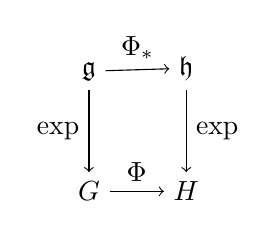
\begin{tikzpicture}
  \matrix (m) [matrix of math nodes, row sep=3em, column sep=2em, minimum width=1em]
  {
 \mathfrak{g}  &   \mathfrak{h}      \\
G     &   H   \\ };
%  \path[-stealth]
\path[->]
  (m-1-1) edge node [above] {$\Phi_*$} (m-1-2)
edge node [left] {$\exp$} (m-2-1)
(m-1-2) edge node [auto] {$\exp$} (m-2-2)
  (m-2-1) edge node [auto] {$\Phi$} (m-2-2);
\end{tikzpicture}

\item[(h)] flow $\theta$ of left-invariant vector field $X$, $\theta_t = R_{\exp{tX}}$
\end{enumerate}
\end{proposition}

\begin{proof}
\begin{enumerate}
\item[(a)]
\item[(b)]
\item[(c)]
\item[(d)]
\item[(e)] Let $X\in \mathfrak{g}$ arbitrary, let $\begin{aligned} & \quad \\ 
  & \sigma: \mathbb{R} \to \mathfrak{g} \\
  & \sigma(t) = tX \\
  & \dot{\sigma}(0) = X \end{aligned}$




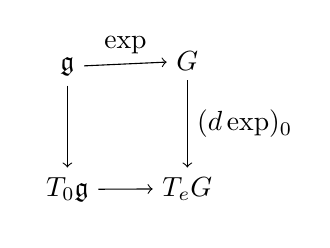
\begin{tikzpicture}
  \matrix (m) [matrix of math nodes, row sep=3em, column sep=2em, minimum width=1em]
  {
 \mathfrak{g}  &   G      \\
T_0\mathfrak{g}     &   T_eG   \\ };
%  \path[-stealth]
\path[->]
  (m-1-1) edge node [above] {$\exp$} (m-1-2)
edge node [left] {$$} (m-2-1)
(m-1-2) edge node [auto] {$(d\exp)_0$} (m-2-2)
  (m-2-1) edge node [auto] {$$} (m-2-2);
\end{tikzpicture}

\[
(d\exp )_0(X) = (d\exp )_0(\dot{\sigma}(0)) = (\exp \circ \sigma)'(0) = (\exp{ (tX)})'(0) = \left. \frac{d}{dt} \right|_{t=0} \exp{ (tX)}= X
\]
\item[(f)] $(d\exp )_0 =1$ and so by inverse function thm., $\exists \, (d\exp)_0^{-1}=1^{-1}=1$, and so $\begin{aligned} & \quad \\
  & U \ni 0 \\
  & U \subseteq \mathfrak{g} \end{aligned} \xrightarrow{ \simeq } \begin{aligned} & \quad \\ 
  & V \ni e \\
  & V \subseteq G \end{aligned}$
\end{enumerate}









\end{proof}



\section{Quotient Manifolds}

\subsection*{ Problems }

\problemhead{21-6}

Suppose Lie group $G$ acts smoothly, freely, and properly on smooth manifold $M$


\section{Symplectic Manifolds}


\subsection{Symplectic Tensors}

\exercisehead{22.1}

{\scriptsize{\url{http://math.stackexchange.com/questions/342267/non-degenerate-bilinear-forms-and-invertible-matrices}}} (shout out to Branimir Cacic for the answer)  gave me a hint at how to approach this exercise, even though the original question was for symmetric bilinear forms.  

Let $\lbrace e_1 \dots e_n \rbrace$ be (some) basis of $V$ \\
Let $\lbrace f^1 \dots f^n \rbrace$ be dual basis of $V$ s.t. $f^i(e_j)=\delta^i_{ \,\, j}$

Now
\[
\begin{aligned}
  & \widehat{\omega}(e_i) = (\widehat{\omega}(e_i))_jf^j \\
  & \widehat{\omega}(e_i)e_j = (\widehat{\omega}(e_i))_j = i_{e_i}\omega(e_j) = \omega(e_i,e_j) \equiv \omega_{ij}
\end{aligned}
\]
so $\omega_{ij} = (\widehat{\omega}(e_i))_j$ (i.e. matrix $\omega_{ij}$ is precisely $(\widehat{\omega}(e_i))_j$.  

If $\omega_{ij}$ nonsingular, i.e. $\exists \, \omega^{-1}_{ki}$ s.t. $\omega^{-1}_{ki} \omega_{ij} = \omega_{ki}\omega^{-1}_{kj} = \delta_{kj}$ (by def.)

If $\widehat{\omega}$ invertible, $\widehat{\omega}^{-1} \widehat{\omega}(v) = v$
\[
\begin{gathered}
  \widehat{\omega}^{-1}\widehat{\omega}(e_i) = \widehat{\omega}^{-1}(\widehat{\omega}(e_i))_j f^j = (\widehat{\omega}(e_i))_j \widehat{\omega}^{-1}(f^j) = (\widehat{\omega}(e_i))_j(\widehat{\omega}^{-1}(f^j))^k e_k = e_i \\
\Longrightarrow (\widehat{\omega}(e_i))_j(\widehat{\omega}^{-1}(f^j))^k = \delta_i^{ \, \, k}
\end{gathered}
\]
So if $\omega_{ij}$ nonsingular, $(\widehat{\omega}^{-1}(f^j))^k$ exists and $(\widehat{\omega}(f^j))^k = \omega^{-1}_{jk}$ \\
\phantom{So } if $\widehat{\omega}$ invertible, $\omega^{-1}_{jk}$ exists and is given by $\omega^{-1}_{jk} = (\widehat{\omega}(f^j))^k$


So the (a) $\Longleftrightarrow$(c) part of the exercise is done.  

Show (a) $\Longleftrightarrow$(b) and we're done.

If $\widehat{\omega}:V\to V^*$ linear isomorphism,  
\[
\text{ker}\widehat{\omega}=0
\]

Suppose $\nexists \, w \in V$ s.t. $\omega(v,w)\neq 0$ (proof by contradiction strategy) \\
Then $\forall \, w \in V$, $\omega(v,w) =0$  \\
$\omega(v,w) = 0 = \widehat{\omega}(v)(w) \quad \, \forall \, w \in V$.  \\
Then $v=0$.  Contradiction.  

(b) $\Longrightarrow $ (a): if $\forall \, v \neq 0$, $\exists \, w \in V$ s.t. $\omega(v,w) \neq 0$ \\
then if $\forall \, w \in V$, $\omega(v,w) =0$, then $v=0$ \\
$\omega(v,w) = \widehat{\omega}(v)(w) = 0$ implies $v=0$, $\forall \, w \in V$.  \\
Then $\text{ker}\widehat{\omega}=0$.  So $\widehat{\omega}$ linear isomorphism.  So $\omega$ nondegenerate.  

\exercisehead{22.4} There was a proof of this in Konstantin Athanassopoulos, \textbf{Notes on Symplectic Geometry}, Iraklion, 2013
\url{http://www.math.uoc.gr/~athanako/symplectic.pdf}

Recall that \\
$S^{\perp} = \lbrace v \in V | \omega(v,w) =0 \quad \, \forall \, w \in S \rbrace$ \\
$(S^{\perp})^{\perp} = \lbrace u \in V | \omega(u,v)=0 \quad \, \forall \, v \in S^{\perp}\rbrace$

Let $s\in S$.  $\omega(s,v)=0 \quad \, \forall \, v \in S^{\perp}$, by def. of $S^{\perp}$ \\
$\begin{aligned} & \quad \\
  & s\in (S^{\perp})^{\perp} \\ 
  \Longrightarrow & S \subseteq (S^{\perp})^{\perp} \end{aligned}$

Then $\text{dim}S \leq \text{dim}(S^{\perp})^{\perp}$ with equality iff $S= (S^{\perp})^{\perp}$

Now by Lemma 22.3, \\
$\text{dim}S + \text{dim}S^{\perp} = \text{dim}V$, $\forall \, $ linear subspace $S\subseteq V$ \\
$\text{dim}S^{\perp} + \text{dim}(S^{\perp})^{\perp} = \text{dim}V = \text{dim}S + \text{dim}S^{\perp} \Longrightarrow \text{dim}S = \text{dim}(S^{\perp})^{\perp}$ \\
 
$\text{dim}S \leq \text{dim} (S^{\perp})^{\perp}$ with equality iff $S= (S^{\perp})^{\perp}$




\subsection{Symplectic Structures on Manifolds}

\exercisehead{22.10} $F:N\to M$ smooth immersion.  Recall definition: $F_*$ injective.  Recall Appendix B, Exercise B.22 (EY: 20150512 This exercise is \textbf{very useful}; I can't emphasize that enough).  $F_*$ injective so $\text{rank}F_* = \text{dim}N$. (implying $\text{ker}F_*=0$).  

Recall that $F$ isotropic if \\

$(F_*)_p(T_pN) \subseteq T_{F(p)}M$ isotropic, i.e. 

\[
(F_*)_p(T_pN) \subseteq ((F_*)_p(T_pN))^{\perp}
\]

Consider $X,Y \in T_pN$, with $X,Y$ nonzero.  Then, as $F_*$ injective, $Z,W \in ((F_*)_p(T_pN))$ nonzero, for $\begin{aligned}
& \quad \\
  & Z = (F_*)_pX \\
  & W = (F_*)_pY \end{aligned}$

Suppose $\omega(Z,W)=0$, $\forall \, W \in (F_*)_p(T_pN)$.  $Z \in ((F_*)_p(T_pN))^{\perp}$.  

\[
\omega(Z,W) = \omega((F_*)_pX, (F_*)_pY) = (F^*)_p\omega(X,Y)=0
\]

If $F$ isotropic, then this is the case $\forall \, Z \in ((F_*)_p(T_pN)) \subseteq ((F_*)_p(T_pN))^{\perp}$.  

Then since $(F^*)_p\omega(X,Y)=0$ \, $\forall \, p \in N$, $\forall \, X,Y \in T_pN$, then $F^*\omega=0$.  

If $F$ symplectic, $(F_*)_p(T_pN) \cap ((F_*)_p(T_pN))^{\perp}=0$

Likewise, for the reverse.  

If $F$ symplectic, 

\[
(F_*)_p(T_pN) \cap ((F_*)_p(T_pN))^{\perp}=0
\]
For $ X,Y \in T_pN$, suppose

\[
F_p^*\omega(X,Y) = \omega((F_*)_pX, (F_*)_pY) =0 
\]

This implies $(F_*)_pX \in (F_*)_p(T_pN) \cap ((F_*)_p(T_pN))^{\perp}$

Then 

since $F_*$ immersion, $X,Y=0$.  So $F^*\omega$ is nondegenerate and so is a symplectic form.  


\subsubsection{the Canonical Symplectic Form on the Cotangent Bundle}

\begin{quote}
The most important symplectic manifolds are total spaces of cotangent bundles, which carry canonical symplectic structures that we now define.
\end{quote}


\subsection{The Darboux Theorem}

\subsection{Hamiltonian Vector Fields}

\textbf{Hamiltonian vector field} of $f$
\[
X_f = \widehat{\omega}^{-1}(df)
\]

Hamiltonian vector field of $f$ in Darboux coordinates:
\begin{equation}
  X_f = \sum_{i=1}^n \left( \frac{ \partial f}{ \partial y^i} \frac{ \partial }{ \partial x^i } - \frac{ \partial f}{ \partial x^i} \frac{\partial}{ \partial y^i} \right)
\end{equation}
(22.9)



smooth $X \in \mathfrak{X}(M)$ \textbf{symplectic} if $\omega$ invariant under flow of $X$, i.e. $\mathcal{L}_X \omega =0$


\subsubsection{Poisson Brackets}

$f \in C^{\infty}(M)$ \textbf{conserved quantity} if $f$ constant on every integral curve of $X_H$.  

smooth $V \in \mathfrak{X}(M)$ \textbf{infinitesimal symmetry} of $(M,\omega,H)$ if $\omega,H$ invariant under flow of $V$, i.e. EY (20150521) 
\[
\begin{aligned}
  & \mathcal{L}_V \omega = 0
  & \mathcal{L}_V H = 0
\end{aligned}
\]

\begin{proposition}[22.21]
Let $(M,\omega,H)$ Hamiltonian system
\begin{enumerate}
\item[(a)] $f \in C^{\infty}(M)$ conserved quantity iff $\lbrace f,H\brace =0$
\item[(b)] infinitesimal symmetries of $(M, \omega,H)$ are precisely symplectic fields $V$ s.t. $VH=0$ 
\item[(c)] if $\theta$ flow of infinitesimal symmetry and $\gamma$ trajectory of system
\end{enumerate}
\end{proposition}

\begin{proof}
This is the solution to Problem 22-18.  

\begin{enumerate}
\item[(a)] if $f\in C^{\infty}(M)$ conserved quantity, by def. $f$ constant on every integral curve of $X_H$
\[
\lbrace f,H\rbrace = \frac{ \partial f}{ \partial x^i} \frac{ \partial H}{ \partial y^i} - \frac{ \partial f}{ \partial y^i} \frac{ \partial H}{ \partial x^i} = X_H f = 0 
\]
for 
\[
X_H = \frac{ \partial H}{ \partial y^i} \frac{ \partial }{ \partial x^i} - \frac{ \partial H}{ \partial x^i} \frac{ \partial }{ \partial y^i} 
\] 
likewise, if $\lbrace f,H \rbrace =0$, then $X_Hf =0$, $X_Hf = \mathcal{L}_{X_H} f= 0 $, so $f$ constant on flow of $X_H$
\item[(b)] Recall smooth $V \in \mathfrak{X}(M)$ infinitesimal symmetry of $(M,\omega,H)$ if $\omega, H$ invariant under flow of $V$, i.e. 
\[
\begin{aligned}
  & \mathcal{L}_V \omega =0 
  &  \mathcal{L}_VH = 0 
\end{aligned}
\]
smooth $V\in \mathfrak{X}(M)$ symplectic if $\omega$ invariant under flow of $V$, i.e. $\mathcal{L}_V\omega =0$
\[
\mathcal{L}_VH = VH = 0
\]
\item[(c)] EY : 20150521 I'm not sure how to go about this because what is a trajectory?

$\gamma: I \to M$

$\theta$ flow of an infinitesimal symmetry, so (collecting facts)

\[
\begin{aligned}
  & \mathcal{L}_{\dot{\theta}}\omega = di_{\dot{\theta}}\omega + i_{\dot{\theta}}d\omega = di_{\dot{\theta}}\omega \quad \, (\omega \text{ closed so } i_{\dot{\theta}}d\omega) \\ 
  & \dot{\theta}H = 0 
\end{aligned}
\]

Now $\theta_s \circ \gamma : I \to M$

\[
\frac{d}{dt}(\theta_s \circ \gamma)(t) = (D\theta_s)(\gamma(t)) \dot{\gamma}(t) = V_{s,\gamma(t)} \dot{\gamma}(t)
\]
\end{enumerate}
\end{proof}

\problemhead{22.1} 

\begin{proof}
\begin{enumerate}
  \item[(a)] If $S$ symplectic, $S \cap S^{\perp} = 0$.  $S=(S^{\perp})^{\perp}$ so $(S^{\perp})^{\perp} \cap S^{\perp} =0$.  $S^{\perp}$ symplectic.  \\
If $S^{\perp}$ symplectic, $S^{\perp} \cap (S^{\perp})^{\perp} = 0$.  $S=(S^{\perp})^{\perp}$ so $(S^{\perp})^{\perp} =S \cap S^{\perp} =0$.  $S$ symplectic.  \\
  \item[(b)] Suppose for $s\in S\cap S^{\perp}$, $s\neq 0$.  Then as $s\in S^{\perp}$, $\omega(s,w)=0 \, \forall \, \, w \in S^{\perp}$. 

Then $\omega(s,s)=0$.  But $\omega$ nondegenerate so $s=0$.  Contradiction.  

Suppose $S$ symplectic.  For $\left. \omega \right|_S(s,t) = \omega(s,t)=0$, for some $s \in S$, $\forall \, t \in S$, then $S\cap S^{\perp}=0$ implies that $s,t=0$.  Then $\left. \omega \right|_S$ nondegenerate.  


  \item[(c)] If $S$ isotropic, $S\subseteq S^{\perp}$ so that $\omega(s,t)=0$ \, $\forall \, t \in S$ (def. of $S^{\perp}$).  $\left. \omega \right|_S =0$ as $\omega(s,t)=0$, \, $\forall \, s,t \in S$.  

If $\left. \omega \right|_S =0$, then $\forall \, s,t \in S$, $\omega(s,t)=0 \, \, \forall \, t\in S$.  By def. of $S^{\perp}$, $S\subseteq S^{\perp}$.  
  \item[(d)] if $S$ coisotropic, $S\supseteq S^{\perp}$.  $S^{\perp} \subseteq S=(S^{\perp})^{\perp}$.  Then $S^{\perp}$ isotropic.  

If $S^{\perp}$ isotropic, $S^{\perp} \subseteq (S^{\perp})^{\perp} = S$, so $S$ coisotropic.  
  \item[(e)] If $S$ Lagrangian, $\forall \, s \in S$, $s\in S^{\perp}$, so that $\omega(s,t) = 0$ \, $\forall \, t \in S$.  Then $\left. \omega \right|_S =0$, (i.e. identically $0$).  \\

$\text{dim}S + \text{dim}S^{\perp} = 2\text{dim}S = \text{dim}V $ by Lemma 22.3, so $\text{dim}S = \frac{1}{2} \text{dim}V$.  

If $\text{dim}S = \frac{1}{2} \text{dim}V$, $\text{dim}S^{\perp} = \frac{1}{2} \text{dim}V = \text{dim}S$.  $\left. \omega \right|_S =0$, so $S$ isotropic, i.e. $S\subseteq S^{\perp}$.  $\text{dim}S \leq \text{dim}S^{\perp}$, with equality iff $S=S^{\perp}$.  
\end{enumerate}
\end{proof}



\problemhead{22.-17} Given Hamiltonian system $(T^*Q, \omega,E)$.  

Recall that 
\[
\begin{aligned}
  q(t) & = (q_1^1(t),q_1^2(t), q_1^3(t) \dots q^1_n(t),q_n^2(t),q_n^3(t))=0 \\
  & = (q^1(t) \dots q^{3n}(t))
\end{aligned}
\]

Now $p(t) = (p_1^1,p_1^2,p_1^3\dots p_n^1,p_n^2,p_n^3)$ and \\
$p_i(t)=M_{ij}\dot{q}^j(t)$ with 

$M_{ij}$ $3n \times 3n$ diagonal matrix $(m_1,m_1,m_1,m_2,m_2,m_2 \dots m_n, m_n, m_n)$

Now $E \in C^{\infty}(T^*Q)$ where 
\[
E(q,p) = V(q) + K(p) = V(q) + \frac{1}{2} M^{ij}p_i p_j
\]

\begin{enumerate}
\item[(a)] Let $\mathbf{u} = (u^1,u^2,u^3)$ 

\[
\begin{aligned}
  & P : T^*Q \to \mathbb{R} \\ 
  & \begin{aligned} P(q,p) & = \mathbf{u}\cdot \mathbf{p}_1 + \mathbf{u}\cdot \mathbf{p}_2 \\ 
      & = u^1p_1^1 + u^2p_1^2 + u^3 p_1^3 +u^1p_2^1 + u^2 p_2^2 + u^3 p_2^3 \end{aligned}
\end{aligned}
\]

 Recall Prop. 22.21, Let $(M,\omega, H)$ Hamiltonian system
\begin{enumerate}
\item[(a)] $f \in C^{\infty}(M)$ conserved quantity iff $\lbrace f, H\rbrace =0$
\end{enumerate}

Now in Darboux coordinates,
\[
\lbrace f, g \rbrace = \sum_{i=1}^n \frac{ \partial f}{ \partial x^i} \frac{ \partial g}{ \partial y^i } - \frac{ \partial f}{ \partial y^i } \frac{ \partial g}{ \partial x^i}
\]
(22.16)

For 
\[
E = V(|\mathbf{q}_2 - \mathbf{q}_1|) + \frac{1}{2} M^{ij}p_ip_j
\]

note that 

\[
\begin{aligned}
  & V(| \mathbf{q}_2 - \mathbf{q}_1|) = V(r) \text{ with } \\ 
  & r = \sqrt{ (q_2^1 - q_1^1)^2 + \dots + (q_2^3 - q_1^3)^2 } \\ 
  & \frac{ \partial V}{ \partial q_i^j} = \frac{ \partial V}{ \partial r} \frac{1}{2} \frac{1}{r}(2)(q_2^j - q_1^j)(-1)^i = \frac{ \partial V}{ \partial r} \frac{1}{r} (q_2^j-q_1^j)(-1)^i
\end{aligned}
\]



then
\[
\begin{aligned}
  & \frac{ \partial E}{ \partial p_i^j} = \frac{p_i^j}{m_i} \\ 
  & \frac{ \partial E}{ \partial q_i^j} = \frac{ \partial V}{ \partial r} \frac{1}{r}(-1)^i (q_2^j-q_1^j)
\end{aligned}
\]
with $r = |\mathbf{q}_2 - \mathbf{q}_1| = \sqrt{ (q_2^1- q_1^1)^2 + \dots + (q_2^3- q_1^3)^2 }$

\[
P = \mathbf{u}\cdot (\mathbf{p}_1 + \mathbf{p}_2) = u^i p^i_1 + u^i p_2^i
\]
\[
\begin{aligned}
\frac{ \partial P}{ \partial p_i^j} = u^j  \\ 
 \frac{ \partial P}{ \partial q }=  0
\end{aligned}
\]

\[
\lbrace P,E \rbrace =0 - u^j \frac{ \partial V}{ \partial r} \frac{1}{r} (-1)^i(q_2^j-q_1^j) = -\mathbf{u}\cdot(\mathbf{q}_2-\mathbf{q}_1) \frac{ \partial V}{ \partial r} \frac{1}{r}(-1) + -\mathbf{u}\cdot (\mathbf{q}_2-\mathbf{q}_1) \frac{ \partial V}{ \partial r} \frac{1}{r} = 0 
\]

\item[(b)] 
\[
L(q,p) = q_1^1 p_1^2 - q_1^2 p_1^1 + q_2^1p_2^2 - q_2^2 p_2^1 
\]
\[
\begin{aligned}
  & \frac{ \partial L}{ \partial q_i^j } = p_i^k \epsilon^{jk} \\ 
  & \frac{ \partial L}{ \partial p_i^k } = q_i^j \epsilon^{jk}
\end{aligned}
\]


\[
\begin{gathered}
  \lbrace L, E \rbrace = p_i^k \epsilon^{jk} \frac{p_i^j}{m_i} - q_i^k \epsilon^{kj} \frac{ \partial V}{ \partial r} \frac{1}{r} (-1)^i (q_2^j - q_1^j) = \frac{ p_i^2 p_i^1}{m_i} - \frac{ p_i^1 p_i^2}{m_i} -  q_i^k \epsilon^{kj} \frac{ \partial V}{ \partial r} \frac{1}{r} (-1)^i (q^j_2 - q^j_1) = \\
  = 0 - \frac{ \partial V}{ \partial r} \frac{1}{r} ( -q_1^2(q_2^1- q_1^1 )(-1) + q_1^1 (q_2^2 - q_1^2)(-1) - q_2^2 (q_2^1 - q_1^1) + q_2^1 (q_2^2 - q_1^2) ) = 0 
\end{gathered}
\]



\end{enumerate}


\problemhead{22-18}

\begin{enumerate}
\item[(a)] if $f\in C^{\infty}(M)$ conserved quantity, by def. $f$ constant on every integral curve of $X_H$
\[
\lbrace f,H\rbrace = \frac{ \partial f}{ \partial x^i} \frac{ \partial H}{ \partial y^i} - \frac{ \partial f}{ \partial y^i} \frac{ \partial H}{ \partial x^i} = X_H f = 0 
\]
for 
\[
X_H = \frac{ \partial H}{ \partial y^i} \frac{ \partial }{ \partial x^i} - \frac{ \partial H}{ \partial x^i} \frac{ \partial }{ \partial y^i} 
\] 
likewise, if $\lbrace f,H \rbrace =0$, then $X_Hf =0$, $X_Hf = \mathcal{L}_{X_H} f= 0 $, so $f$ constant on flow of $X_H$
\item[(b)] Recall smooth $V \in \mathfrak{X}(M)$ infinitesimal symmetry of $(M,\omega,H)$ if $\omega, H$ invariant under flow of $V$, i.e. 
\[
\begin{aligned}
  & \mathcal{L}_V \omega =0 
  &  \mathcal{L}_VH = 0 
\end{aligned}
\]
smooth $V\in \mathfrak{X}(M)$ symplectic if $\omega$ invariant under flow of $V$, i.e. $\mathcal{L}_V\omega =0$
\[
\mathcal{L}_VH = VH = 0
\]
\item[(c)] EY : 20150521 I'm not sure how to go about this because what is a trajectory?

$\gamma: I \to M$

$\theta$ flow of an infinitesimal symmetry, so (collecting facts)

\[
\begin{aligned}
  & \mathcal{L}_{\dot{\theta}}\omega = di_{\dot{\theta}}\omega + i_{\dot{\theta}}d\omega = di_{\dot{\theta}}\omega \quad \, (\omega \text{ closed so } i_{\dot{\theta}}d\omega) \\ 
  & \dot{\theta}H = 0 
\end{aligned}
\]

Now $\theta_s \circ \gamma : I \to M$

\[
\frac{d}{dt}(\theta_s \circ \gamma)(t) = (D\theta_s)(\gamma(t)) \dot{\gamma}(t) = V_{s,\gamma(t)} \dot{\gamma}(t)
\]
\end{enumerate}









\begin{appendix}


\section{Review of Topology}

\subsection*{Topological Spaces}

\begin{itemize}
  \item \textbf{neighborhood of $p$} open subset $\mathcal{O}$ containing $p$
\end{itemize}



\subsubsection*{Bases and Countability}

Suppose $X$ topological space.

\textbf{basis for topology of $X$ } \[
\mathcal{B} = \lbrace B | \text{ open } B \subseteq X, \, \forall \,  \text{ open } \mathcal{O} \subset X, \, \mathcal{O} = \bigcup_{\alpha} B_{\alpha} \rbrace
\]

\textbf{neighborhood basis at $p$ } $\mathcal{B}_p = \lbrace \text{neighborhoods } B_p \text{ of $p$ } | \forall \, \mathcal{O} \text{ of } p,  B_p \subset \mathcal{O}, \, B_p \in \mathcal{B}_p \text{ for at least 1 } \rbrace$

$X$ \textbf{first countable }- if $\exists \, $ countable neighborhood basis $\forall \, p$

\textbf{second countable } if $\exists \, $ countable basis

\begin{proposition}[A.16]  Let $X$ second countable topological space. \\
$\forall \, $ open cover of $X$ has countable subcover
\end{proposition}

\begin{proof}
  $X$ second countable. $\exists \, $ countable basis $\mathcal{B}$ for $X$ \\
Let $\mathcal{U}$ arbitrary open cover of $X$. \\
Let $\mathcal{B}' \subseteq \mathcal{B}$ s.t. $\mathcal{B}' = \lbrace  B | B \in \mathcal{B}, B\subseteq U \text{ for some } U \in \mathcal{U} \rbrace$ \\

$\forall \, B \in \mathcal{B}'$, choose particular $U_B \in \mathcal{U}$ containing $B$ \\

$\lbrace U_B | B \in \mathcal{B}'\rbrace$ countable \\

$\forall \, x \in X$ , $\exists \, V \in \mathcal{U}$, $x\in V$ \\
$\mathcal{B} $ basis, s.t. $\exists \, B \in \mathcal{B}$ s.t. $x\in B \subseteq V$ \\
then $B \in \mathcal{B}'$, so $x\in B \subseteq U_B$
\end{proof} 

\subsection*{Subspaces, Products, Disjoint Unions, and Quotients }

% AReviewofTopology.tex
% Fund Science! & Help Ernest finish his Physics Research! : quantum super-A-polynomials - a thesis by Ernest Yeung
%                                               
% http://igg.me/at/ernestyalumni2014                                                                             
%                                                              
% Facebook     : ernestyalumni  
% github       : ernestyalumni                                                                     
% gmail        : ernestyalumni                                                                     
% google       : ernestyalumni                                                                                   
% linkedin     : ernestyalumni                                                                             
% tumblr       : ernestyalumni                                                               
% twitter      : ernestyalumni                                                             
% youtube      : ernestyalumni                                                                
% indiegogo    : ernestyalumni                                                                        
%
% Ernest Yeung was supported by Mr. and Mrs. C.W. Yeung, Prof. Robert A. Rosenstone, Michael Drown, Arvid Kingl, Mr. and Mrs. Valerie Cheng, and the Foundation for Polish Sciences, Warsaw University.                  

\section*{Review of Topology}

\subsection*{Topological Spaces}

Let $X$ set \\
topology on $X = $ collection $\tau = \lbrace U | U \subseteq X \rbrace$, $U$ called open subsets s.t.
\begin{enumerate}
\item[(i)] $X, \emptyset$ open 
\item[(ii)] $\bigcup_{\alpha} U_{\alpha}$ is open, $\forall \, U_{\alpha}$ open subset
\item[(iii)] $\bigcap_{i=1}^n U_i$ is open
\end{enumerate}

$(X,\tau)$ topological space


\textbf{Example A.5. (Metric Spaces)}
metric space $=$ set $M$ with metric $d: M \times M \to \mathbb{R}$ s.t. $\forall \, x, y, z \in M$
\begin{enumerate}
\item[(i)] \textsc{Positivity} $d(x,y) \geq 0$, $d(x,y) =0$ iff $x=y$ 
\item[(ii)] \textsc{Symmetry} $d(x,y) =d(y,x)$
\item[(iii)] \textsc{Triangle inequality} $d(x,z) \leq d(x,y) + d(y,z)$
\end{enumerate}

if $M$ metric space, $x\in M$, $r>0$ \\
\phantom{\quad } \textbf{open ball of radius $r$ around $x$ } 
\[
B_r(x) = \{ y \in M | d(x,y) < r \}
\]
\phantom{\quad \quad } \textbf{closed ball of radius $r$ }
\[
\underline{B}_r(x) = \{ y \in M | d(x,y) \leq r \}
\]
\textbf{metric topology on $M$ } defined by declaring $S \subseteq M$ open iff $\forall \, x \in S$, $\exists \, r >0$ s.t. $B_r(x) \subseteq S$



% BReviewofLinearAlgebra.tex
% Fund Science! & Help Ernest finish his Physics Research! : quantum super-A-polynomials - a thesis by Ernest Yeung
%                                               
% http://igg.me/at/ernestyalumni2014                                                                             
%                                                              
% Facebook     : ernestyalumni  
% github       : ernestyalumni                                                                     
% gmail        : ernestyalumni                                                                     
% google       : ernestyalumni                                                                                   
% linkedin     : ernestyalumni                                                                             
% tumblr       : ernestyalumni                                                               
% twitter      : ernestyalumni                                                             
% youtube      : ernestyalumni                                                                
% indiegogo    : ernestyalumni                                                                        
%
% Ernest Yeung was supported by Mr. and Mrs. C.W. Yeung, Prof. Robert A. Rosenstone, Michael Drown, Arvid Kingl, Mr. and Mrs. Valerie Cheng, and the Foundation for Polish Sciences, Warsaw University.                  



\section{Review of Linear Algebra }

\subsection{Linear Maps}

\exercisehead{B.1}
\begin{enumerate}
  \item[(a)]
\item[(b)]
\item[(c)]
\item[(d)] \textbf{Want}: if $(v_1 \dots v_k)$ linearly dependent $k$-tuple in $V$, $v_1 \neq 0$, \\
then some $v_i = \sum_{j=1}^{i-1} c^j v_j$ \\
\begin{proof}
$(v_1 \dots v_k)$ linearly dependent, so if $\sum_{i=1}^k a^i v_i = 0$, $a^i$ not all equal to $0$.  \\

Suppose for fixed $i$, $2\leq i \leq k$, $a^{i+1} = \dots =a^k=0$. \\
\quad Indeed, suppose for $\sum_{i=1}^k a^i v_i = 0$, $a^2 = \dots = a^k = 0$.  $a^1 v_1 =0$, $v_1 \neq 0$, $a^1 =0$.  Then $(v_1 \dots v_k)$ linearly independent.  Contradiction.  

if $i=2$, \\
\phantom{\quad} $a^1 v_1 + a^2 v_2 =0$ \\
\phantom{\quad \,} $\Longrightarrow v_2  = \frac{-a^1}{a^2} v_1$ \\

if $i=k$, $v_k = \frac{ -\sum_{i=1}^{k-1} a^i v_i }{ a^k}$  \\

So in general, $v_i = \frac{ -\sum_{j=1}^{i-1} a^j v_j }{ a^i}$
\end{proof}
\end{enumerate}

\exercisehead{B.9}
given $(E_1 \dots E_n)$ basis for $V$ \\
\phantom{ \quad } $\exists \, \lbrace i_1 \dots i_k \rbrace \subset \lbrace 1 \dots n \rbrace$ s.t. \\
\phantom{ \quad \, } $ \text{span}(E_{i_1} \dots E_{i_k} )$ is complement to $S$ \\

Hence $\forall \, $ subspace $S \subseteq V$, $\exists \, $ complementary subspace $T$ in $V$, so $V = S \oplus T$

\begin{proof}
$\forall \, $ subspace $S$ is itself a vector space, closed under addition and multiplication. \\
\phantom{ \quad } Hence $S$ has basis $(F_1 \dots F_m)$ with $\text{dim}S = m$ \\

Consider ordered $(m+n)$-tuple 
\[
(F_1 \dots F_m, E_1 \dots E_n)
\]

$(F_1 \dots F_m, E_1 \dots E_n)$ linearly dependent in $V$, by linear algebra. 

For $j_1 \in \lbrace 1 \dots n \rbrace$, $E_{j_1}$ linear combination of previous vectors (cf. Exercise B.1(d)) \\
\phantom{ \quad } eliminate $E_{j_1}$ : $(F_1 \dots F_m, E_1 \dots \widehat{E}_{j_1} \dots E_n )$. \\

Repeat, until there are $n-m$ $E$ basis vectors left, labeled $i_1 \dots i_{n-m}$ (hence \textbf{use Exercise B.1(d)} many and enough times, $m$ times)
\[
\Longrightarrow (F_1 \dots F_m, E_{i_1} \dots E_{i_{n-m}} )
\]
By linear algebra, $(F_1 \dots F_m, E_{i_1} \dots E_{i_{n-m}})$ a basis for $V$, linearly independent. The procedure wouldn't have ``overshot'' by a Thm. (see Apostol's \textbf{Calculus} Vol. 2, first few chapters, linear algebra part) \\

$\forall \, v\in V$, $v= a^iF_i  + b^{i_j} E_{i_j}$ with $a^i F_i \in S$.  Then $b^{i_j} E_{i_j} \in T$.  \\
\phantom{ \quad } since $V = S\oplus T$, $T$ complement to $S$

$\Longrightarrow $ given fixed basis of $V$, $(E_1 \dots E_n)$, subspace $S \subseteq V$, $S$ having basis $(F_1 \dots F_m)$, $S$ has complementary subspace in $V$, $T$, \\
\phantom{ \quad } s.t. basis of $T$ is $(E_{i_1} \dots E_{i_{n-m}})$ and $V = S\oplus T$

\end{proof}


\exercisehead{B.13}  Suppose $\exists \, $ linear $T: V \to W $ s.t. $T(E_i) = w_i$, \quad \, $i = 1 \dots n$ \\
Suppose $\exists \, $ linear $T':V \to W$ s.t. $T'(E_i)= w_i$, \quad \, $i = 1 \dots n$

Let $x\in V$, so $x  = x^i E_i$ (the key idea is that with a basis, the vector space is completely determined, vectors in the vector space are spanned by the basis elements)
\[
(T-T')(x) \equiv T(x) - T'(x)  = x^i w_i - x^i w_i = 0
\]
$T(x) = T'(x)$\quad \, $\forall \, x \in V$ \\
so $T=T'$.  $T$ unique.  

$T$ exists by construction.
\hrulefill


\textbf{ affine subspace } of $V$ parallel to $S$, linear subspace $S \subseteq V$, $v + S = \lbrace v + w | w \in S \rbrace$, some fixed $v \in V$ \\

\textbf{affine map } $F: V \to W$ if $F(v) = w + Tv$ for some $T: V \to W$, some fixed $w\in W$ \\

\exercisehead{B.16}

Let $a,b \in \mathbb{C}$, $x, y \in F(V)$ \\

Now 
\[
F(V) = \lbrace y | y = w + Tv = F(v), \, v \in V, \text{ fixed } w \in W , \text{ some } T \rbrace
\]

\subsubsection{Change of Basis}




\exercisehead{B.22} Suppose $V,W, X$ finite-dim. vector spaces \\
$S:V\to W$, \, $T:W \to X$

\begin{enumerate}
\item[(a)] $\text{rank}S \leq \text{dim}V$ \quad \, $\text{rank}S = \text{dim}V$ iff $S$ injective
\item[(b)] $\text{rank}S \leq \text{dim}W$ \quad \, $\text{rank}S = \text{dim}W$ iff $S$ surjective
\item[(c)] if $\text{dim}V = \text{dim}W$ and $S$ either injective or surjective, then $S$ isomorphism 
\item[(d)] $\text{rank}TS \leq \text{rank}S$ \quad \, $\text{rank}TS = \text{rank}S$ iff $\text{im}S \bigcap \text{ker}T = 0$ 
\item[(e)] $\text{rank}TS \leq \text{rank}T$ \quad \, $\text{rank}TS = \text{rank}T$ iff $\text{im}S + \text{ker}T = W$
\item[(f)] if $S$ isomorphism, then $\text{rank}TS = \text{rank}T$
\item[(g)] if $T$ isomorphism, then $\text{rank}TS = \text{rank}S$
\end{enumerate}

EY : Exercise B.22(d) is useful for showing the chart and atlas of a Grassmannian manifold, found in the More examples, for smooth manifolds.  

\begin{proof}
\begin{enumerate}
\item[(a)]
\item[(b)]
\item[(c)]
\item[(d)] Now 
\[
\begin{aligned}
  & \text{dim}V = \text{rank}TS + \text{nullity}TS \\ 
  &  \text{dim}V = \text{rank}S + \text{nullity}S
\end{aligned}
\]
$\text{ker}S \subseteq \text{ker}TS$, clearly, so $\text{nullity}S \leq \text{nullity}TS$ 
\[
\Longrightarrow \boxed{ \text{rank}TS \leq \text{rank}S } 
\]

If $\text{rank}TS = \text{rank}S$, \\
\phantom{ \quad } then $\text{nullity}S = \text{nullity}TS$ \\
\phantom{ \, } Suppose $w \in \text{Im}S \bigcap \text{ker}T$, $w \neq 0$ \\
\phantom{ \quad } Then $\exists \,  v\in S$, s.t. $w = S(v)$ and $T(w)=0$ \\
\phantom{ \quad \, } Then $T(w) = TS(v) =0$.  So $v\in \text{ker}TS$ \\
\phantom{ \quad \quad \, } $v\notin \text{ker}S$ since $w = S(v) \neq 0$ \\
\phantom{ \quad \quad \, } This implies $\text{nullity}TS > \text{nullity}S$.  Contradiction. \\
$\Longrightarrow \text{Im}S \bigcap \text{ker}T =0$ \\

If $\text{Im}S \bigcap \text{ker}T =0$, \\
\phantom{ \quad } Consider $v \in \text{ker}TS$.  Then $TS(v)=0$.  \\
\phantom{ \quad  Consider $v \in \text{ker}TS$}.  Then $S(v)  \in \text{ker}T$ \\
\phantom{ \quad  } $S(v) =0$; otherwise, $S(v) \in \text{Im}S$, contradicting given $\text{Im}S \bigcap \text{ker}T =0$ \\
\phantom{ \quad \quad } $v\in \text{ker}S$ \\

$\text{ker}TS \subseteq \text{ker}S$\\
$\Longrightarrow \text{ker}TS = \text{ker}S$ \\
So $\text{nullity}TS = \text{nullity}S$  \\
$\Longrightarrow \text{rank}TS = \text{rank}S$ 

\item[(e)]
\item[(f)]
\item[(g)]
\end{enumerate}
\end{proof}



\subsection*{Inner Products and Norms}


\subsubsection*{Norms}

If $V$ real vector space, \\
\phantom{\quad } norm on $V$, $v \mapsto |v| \in \mathbb{R}$ s.t.
\begin{enumerate}
\item[(i)] \textsc{Positivity} $|v| \geq 0$, \, $\forall \, v \in V$, $|v| =0$ iff $v=0$ 
\item[(ii)] \textsc{Homogeneity} $|cv| = |c| |v|$ \quad \, $\forall \, c \in \mathbb{R}$, $v\in V$
\item[(iii)] \textsc{Triangle Inequality} $|v+w | \leq |v| + |w|$, \, $\forall \, v,w \in V$
\end{enumerate}

2 norms $| \, \cdot \, |_1$, $| \, \cdot \, |_2$ on vector space $V$ equivalent if $\exists \, $ constants $c,C >0$ s.t. 
\[
c|v|_1 \leq |v|_2 \leq C|v|_1 \quad \quad \, \forall \, v \in V
\]

\exercisehead{B.49} $\forall \, x \in V$, \\
Consider $B_r(x) = \{ y \in V | |y-x|_2 < r \}$ \\
\phantom{ \quad } Note $y-x \in V$ as $V$ is a vector space

\[
\begin{gathered}
  c|y-x|_1 \leq |y-x|_2 \leq C |y-x|_1 \\ 
 c|y-x|_1 \leq |y-x_2| < r \\
 |y-x|_1 < \frac{r}{c}
\end{gathered}
\]
Now suppose $S \subseteq V$ open in $| \, \cdot \, |_2$ \\
\phantom{ \quad } But $S$ also open in $| \, \cdot \, |_1$ as $\exists \, \frac{r}{c'} >0$ s.t. $B_{\frac{r}{c'}}(x) \subseteq S$ for the exact same pts. as $S$ \\
so $| \, \cdot \, |_1, | \, \cdot \, |_2$ equivalent norms yield the same metric topology.  

EY : 20141220



\subsection*{Direct Products and Direct Sums}





% CReviewofCalculus.tex
% Fund Science! & Help Ernest finish his Physics Research! : quantum super-A-polynomials - a thesis by Ernest Yeung
%                                               
% http://igg.me/at/ernestyalumni2014                                                                             
%                                                              
% Facebook     : ernestyalumni  
% github       : ernestyalumni                                                                     
% gmail        : ernestyalumni                                                                     
% google       : ernestyalumni                                                                                   
% linkedin     : ernestyalumni                                                                             
% tumblr       : ernestyalumni                                                               
% twitter      : ernestyalumni                                                             
% youtube      : ernestyalumni                                                                
% indiegogo    : ernestyalumni                                                                        
%
% Ernest Yeung was supported by Mr. and Mrs. C.W. Yeung, Prof. Robert A. Rosenstone, Michael Drown, Arvid Kingl, Mr. and Mrs. Valerie Cheng, and the Foundation for Polish Sciences, Warsaw University.                  

\section{Review of Calculus}

\subsection*{Total and Partial Derivatives}

\begin{proposition}[C.3] (The Chain Rule for Total Derivatives)

Suppose $V,W,X$ finite-dim. vector spaces

open $\begin{aligned}
  & \quad \\ 
  & U \subseteq V \\
  & \widetilde{U} \subseteq W \end{aligned}$

maps $\begin{aligned}
  & \quad \\
  & F : U \to \widetilde{U} \\
  & G: \widetilde{U} \to X \end{aligned}$

if $F$ diff. at $a\in U$, $G$ diff. at $F(a) \in \widetilde{U}$, \\
\phantom{ \quad } then $GF$ diff. at $a$
\[
D(GF)(a) = DG(F(a)) \circ DF(a)
\]
\end{proposition}

\begin{proposition}[C.4] Suppose $\begin{aligned}
    & \quad \\ 
    & U \subseteq \mathbb{R}^n \\
    & V\subseteq \mathbb{R}^m \end{aligned}$, \quad \, $F: U \to V$ diffeomorphism \\
Then $m=n$ and \\
\phantom{ \quad } $\forall \, a \in U$, $DF(a)$ invertible, with 
\[
DF(a)^{-1} = D(F^{-1})(F(a))
\]
\end{proposition}

\begin{proof}
$F^{-1}F = 1_U$  \\
Chain rule implies $\forall \, a \in U$, 

\begin{equation}
  1_{\mathbb{R}^n} = D(1_U)(a) = D(F^{-1}F)(a) = DF^{-1}(F(a))DF(a) \quad \quad \, (C.5)
\end{equation}

Similarly $FF^{-1}=1_V$ implies
\[
DF(a)DF^{-1}(F(a)) = 1_{\mathbb{R}^m}
\]
so thus
\[
DF(a)^{-1}=D(F^{-1})(F(a))
\]
\end{proof}




\end{appendix}

\end{document}

